% Template for PLoS
% Version 3.4 January 2017
%
% % % % % % % % % % % % % % % % % % % % % %
%
% -- IMPORTANT NOTE
%
% This template contains comments intended
% to minimize problems and delays during our production
% process. Please follow the template instructions
% whenever possible.
%
% % % % % % % % % % % % % % % % % % % % % % %
%
% Once your paper is accepted for publication,
% PLEASE REMOVE ALL TRACKED CHANGES in this file
% and leave only the final text of your manuscript.
% PLOS recommends the use of latexdiff to track changes during review, as this will help to maintain a clean tex file.
% Visit https://www.ctan.org/pkg/latexdiff?lang=en for info or contact us at latex@plos.org.
%
%
% There are no restrictions on package use within the LaTeX files except that
% no packages listed in the template may be deleted.
%
% Please do not include colors or graphics in the text.
%
% The manuscript LaTeX source should be contained within a single file (do not use \input, \externaldocument, or similar commands).
%
% % % % % % % % % % % % % % % % % % % % % % %
%
% -- FIGURES AND TABLES
%
% Please include tables/figure captions directly after the paragraph where they are first cited in the text.
%
% DO NOT INCLUDE GRAPHICS IN YOUR MANUSCRIPT
% - Figures should be uploaded separately from your manuscript file.
% - Figures generated using LaTeX should be extracted and removed from the PDF before submission.
% - Figures containing multiple panels/subfigures must be combined into one image file before submission.
% For figure citations, please use "Fig" instead of "Figure".
% See http://journals.plos.org/plosone/s/figures for PLOS figure guidelines.
%
% Tables should be cell-based and may not contain:
% - spacing/line breaks within cells to alter layout or alignment
% - do not nest tabular environments (no tabular environments within tabular environments)
% - no graphics or colored text (cell background color/shading OK)
% See http://journals.plos.org/plosone/s/tables for table guidelines.
%
% For tables that exceed the width of the text column, use the adjustwidth environment as illustrated in the example table in text below.
%
% % % % % % % % % % % % % % % % % % % % % % % %
%
% -- EQUATIONS, MATH SYMBOLS, SUBSCRIPTS, AND SUPERSCRIPTS
%
% IMPORTANT
% Below are a few tips to help format your equations and other special characters according to our specifications. For more tips to help reduce the possibility of formatting errors during conversion, please see our LaTeX guidelines at http://journals.plos.org/plosone/s/latex
%
% For inline equations, please be sure to include all portions of an equation in the math environment.  For example, x$^2$ is incorrect; this should be formatted as $x^2$ (or $\mathrm{x}^2$ if the romanized font is desired).
%
% Do not include text that is not math in the math environment. For example, CO2 should be written as CO\textsubscript{2} instead of CO$_2$.
%
% Please add line breaks to long display equations when possible in order to fit size of the column.
%
% For inline equations, please do not include punctuation (commas, etc) within the math environment unless this is part of the equation.
%
% When adding superscript or subscripts outside of brackets/braces, please group using {}.  For example, change "[U(D,E,\gamma)]^2" to "{[U(D,E,\gamma)]}^2".
%
% Do not use \cal for caligraphic font.  Instead, use \mathcal{}
%
% % % % % % % % % % % % % % % % % % % % % % % %
%
% Please contact latex@plos.org with any questions.
%
% % % % % % % % % % % % % % % % % % % % % % % %

\documentclass[10pt,letterpaper]{article}
\usepackage[top=0.85in,left=2.75in,footskip=0.75in]{geometry}

% amsmath and amssymb packages, useful for mathematical formulas and symbols
\usepackage{amsmath,amssymb}

% Use adjustwidth environment to exceed column width (see example table in text)
\usepackage{changepage}

% Use Unicode characters when possible
\usepackage[utf8x]{inputenc}

% textcomp package and marvosym package for additional characters
\usepackage{textcomp,marvosym}

% cite package, to clean up citations in the main text. Do not remove.
\usepackage{cite}

% % Added natbib for citet commands:
% \usepackage[numbers]{natbib}

% Added url for urls:
\usepackage{url}

% Use nameref to cite supporting information files (see Supporting Information section for more info)
\usepackage{nameref,hyperref}

% line numbers
\usepackage[right]{lineno}

% ligatures disabled
\usepackage{microtype}
\DisableLigatures[f]{encoding = *, family = * }

% color can be used to apply background shading to table cells only
\usepackage[table]{xcolor}

% array package and thick rules for tables
\usepackage{array}

% create "+" rule type for thick vertical lines
\newcolumntype{+}{!{\vrule width 2pt}}

% create \thickcline for thick horizontal lines of variable length
\newlength\savedwidth
\newcommand\thickcline[1]{%
  \noalign{\global\savedwidth\arrayrulewidth\global\arrayrulewidth 2pt}%
  \cline{#1}%
  \noalign{\vskip\arrayrulewidth}%
  \noalign{\global\arrayrulewidth\savedwidth}%
}

% \thickhline command for thick horizontal lines that span the table
\newcommand\thickhline{\noalign{\global\savedwidth\arrayrulewidth\global\arrayrulewidth 2pt}%
\hline
\noalign{\global\arrayrulewidth\savedwidth}}


% Remove comment for double spacing
%\usepackage{setspace}
%\doublespacing

% Text layout
\raggedright
\setlength{\parindent}{0.5cm}
\textwidth 5.25in
\textheight 8.75in

% Bold the 'Figure #' in the caption and separate it from the title/caption with a period
% Captions will be left justified
\usepackage[aboveskip=1pt,labelfont=bf,labelsep=period,justification=raggedright,singlelinecheck=off]{caption}
\renewcommand{\figurename}{Fig}

% Use the PLoS provided BiBTeX style
\bibliographystyle{plos2015}
% \bibliographystyle{plainnat}

% Remove brackets from numbering in List of References
\makeatletter
\renewcommand{\@biblabel}[1]{\quad#1.}
\makeatother

% Leave date blank
\date{}

% Header and Footer with logo
\usepackage{lastpage,fancyhdr,graphicx}
\usepackage{epstopdf}
\usepackage{hyperref}% http://ctan.org/pkg/hyperref
\pagestyle{myheadings}
\pagestyle{fancy}
\fancyhf{}
\setlength{\headheight}{27.023pt}
\lhead{
\includegraphics[width=2.0in]{PLOS-submission.eps}}
\rfoot{\thepage/\pageref{LastPage}}
\renewcommand{\footrule}{\hrule height 2pt \vspace{2mm}}
\fancyheadoffset[L]{2.25in}
\fancyfootoffset[L]{2.25in}
\lfoot{\sf PLOS}


% Make it so figures are more likely to share a page with text:
\renewcommand{\topfraction}{0.85} % 85% rather than default 70% of the top of a text page can contain figures.
\renewcommand{\textfraction}{0.1} % as little as 10% of a page can be text when shared with a figure.
\renewcommand{\floatpagefraction}{0.80} % only makes a figure-only page if figure takes up more than 75% of a page

%% Include all macros below

\newcommand{\lorem}{{\bf LOREM}}
\newcommand{\ipsum}{{\bf IPSUM}}

%% END MACROS SECTION

\graphicspath{{./figs/}}

\begin{document}
\vspace*{0.2in}

% Title must be 250 characters or less.
\begin{flushleft}
{\Large
\textbf\newline{Hub connectivity and gene expression in the worm connectome} % Please use "sentence case" for title and headings (capitalize only the first word in a title (or heading), the first word in a subtitle (or subheading), and any proper nouns).
}
\newline
% Insert author names, affiliations and corresponding author email (do not include titles, positions, or degrees).
\\
Aurina Arnatkevi\u{c}i\={u}t\.{e}\textsuperscript{1\Yinyang},
Ben D. Fulcher\textsuperscript{1\Yinyang},
Alex Fornito\textsuperscript{1}*\\
\bigskip
\textbf{1} Brain and Mental Health Laboratory, Monash Institute of Cognitive and Clinical Neurosciences, School of Psychological Sciences, Monash University, 770 Blackburn Rd, Clayton, 3168, VIC, Australia.
\\
\bigskip

% Insert additional author notes using the symbols described below. Insert symbol callouts after author names as necessary.
%
% Remove or comment out the author notes below if they aren't used.
%
% Primary Equal Contribution Note
\Yinyang These authors contributed equally to this work.

% Additional Equal Contribution Note
% Also use this double-dagger symbol for special authorship notes, such as senior authorship.
% \ddag These authors also contributed equally to this work.

% Current address notes
% \textcurrency Current Address: Dept/Program/Center, Institution Name, City, State, Country % change symbol to "\textcurrency a" if more than one current address note
% \textcurrency b Insert second current address
% \textcurrency c Insert third current address

% Deceased author note
% \dag Deceased

% Group/Consortium Author Note
% \textpilcrow Membership list can be found in the Acknowledgments section.

% Use the asterisk to denote corresponding authorship and provide email address in note below.
* alex.fornito@monash.edu

\end{flushleft}
% Please keep the abstract below 300 words
\section*{Abstract}
WE $\heartsuit$ CAENORHABDITIS ELEGANS


% Please keep the Author Summary between 150 and 200 words
% Use first person. PLOS ONE authors please skip this step.
% Author Summary not valid for PLOS ONE submissions.
\section*{Author summary}
WE $\heartsuit$ WORMS

\linenumbers

% Use "Eq" instead of "Equation" for equation citations.
\section*{Introduction}

% ALEX:
%
% \begin{itemize}
%     \item Nervous systems are complex
%     \item Complexity commonly studied using graphs
%     \item Generality of graphs allows nervous systems to be modeled using a common framework across scales and species
%     \item This work has shown that nervous systems are modular, has hubs, and hubs are connected forming an RC
%     \item RC important for integration, but also costly
%     % \item In particular, conservation of hub connectivity across scales and species implies genetic influences
%     % \item this has been confirmed in mouse by Fulcher, and human by Vertes (cf. Fornito heritability work)
%     % \item C elegans is attractive model to extend these results as connectome mapped completely at synapse and neuron level. We also have detailed information on neuron birth times, cell lineage, neuron type... etc that can help determine whether genomic similarity is driven by one of these factors
%     % \item In this work, we collated all these diverse data to test hypothesis that elevated expression coupling of hubs would be apparent at microscale, and to identify what specifically drives this result.
% \end{itemize}
%
%
% \begin{enumerate}
%     \item{Structural network properties}
%     \begin{itemize}
%     \item{rich-club, hubs, conservation cross-scale/species/methods}
%     \item{Prior work in worm: different types of connectomes - wired/unwired, hubs}
%     \end{itemize}
%
%     \item{Structure-expression}
%     \begin{itemize}
%     \item{Datasets in different scales: mouse/rat, human (also heritability), developmental, large-scale datasets}
%     \end{itemize}
%  \end{enumerate}


% BF Paragraph 1 (deleted by AF)
% % Introduce the structural connectome, characterization of its properties, focusing on worm, but also linking to other species to make the point of consistency
% Structure in the complex web of the axonal connections between neurons may contain clues to understanding how biological function has evolved from a physical system.
% % under physical and energetic constraints.
% The network of connections, or `connectome', can be represented as a graph, in which neural elements are represented as nodes (e.g., individual neurons, as in \emph{C. elegans}, or macroscopic brain regions, as in human), with edges representing axonal projections from one node to another.
% This representation allows very different species, measurements, and scales of neuronal networks to be represented in a consistent and unified way.
% Comparing connectomes across organisms, from the scale of neurons in model organisms like \emph{C. elegans}, mesoscale brain regions using tract tracing in rodents, to non-invasive MRI imaging in human subjects, has revealed a surprising consistency of organizational properties, suggesting a common set of selection pressures under which efficient neural systems have evolved \cite{vandenHeuvel:2016eg}.
% Connectomes consistently display a number of features, including modular structure a non-uniform distribution of connectivity across the network, containing a small number of highly connected `hub' nodes, features that can only partially be accounted for by spatial constraints \cite{Henderson:2014fg, Roberts:2016il}.
% These hubs have been shown to be strongly and densely interconnected with each other, forming an integrated `rich club' that is costly to develop (containing stronger, longer-distance projections) but delivers functional benefits by facilitating efficient integration of information between more specialized processing modules \cite{VandenHeuvel2012}.
% % Rich-club connectivity has also been shown to be costly to develop, with stronger and longer-distance projections that are thought to deliver functional benefits through the integration of diverse neural systems \cite{VandenHeuvel2012}.
% Prior work has characterized the rich-club organization of the neuronal connectome of the \emph{C. elegans} nervous system \cite{Towlson:2013gf}, \emph{Drosophila} \cite{Shih:2015cu}, mouse \cite{Fulcher:2016ck}, rat \cite{vandenHeuvel:2015ie}, 53 \cite{ZamoraLopez:2010hy} or 65 areas \cite{deReus:2013cy} of the cat cortex, 242 macaque cortical regions \cite{Harriger:2012bb}, and in 82 brain regions \cite{vandenHeuvel:2011he} and 1\,170 human cortical areas \cite{vandenHeuvel:2012kh}.
% The consistency of hubs and rich-club connectivity structural across the connectomes of so many species and scales suggests that it may be subject to genetic control.
% % I DON'T BELIEVE IN THIS ONE SO LEAVING IT OUT: pigeon \cite{Shanahan:2013ej},

Neuronal connectivity provides the substrate for integrated brain function.
Recent years have seen several systematic and large-scale attempts to generative comprehensive wiring diagrams -- connectomes -- of nervous systems in species as diverse as the nematode worm \emph{Caenorhabditis elegans} \cite{White:1986tx, Varshney2011}, the drosophila fruit fly \cite{Chiang:2011, Shih:2015cu}, zebrafish \cite{Wanner:2016ea, Hildebrand:2017iu}, mouse \cite{Oh2014, Zingg:2014el}, rat [[CITE-Swanson]], cat [[CITE--Young]], macaque [[CITE--Stephan]]\cite{Markov:2012wu} and human \cite{Hagmann:2008gda} [[CITE--Van Essen Neuroimage HCP review]].
One of the most striking findings to emerge from analyses of these diverse data, acquired using different measurement techniques and at resolution scales ranging from nm to mm, is of a strong conservation of certain, non-random topological properties of network organization (reviewed in \cite{Bullmore:2009iv, Bullmore:2012vl}; [[CITE--Schroeter et al NRN]]; [[CITE--Sporns Fron Comp Neurosci 2011]]; [[CITE--van den Heuvel Bullmore and Sporns TICS]]; see also \cite{fornito2016book}).
These properties include a modular organization, such that subsets of functionally related (and usually spatially adjacent) elements are densely interconnected with each other;
a hierarchy of modules, such that modules contain nested sub-modules and so on over multiple scales (\cite{Meunier:2010hq}[[CITE--Basset-PlosCompBiol]]);
economical connectivity, such that wiring costs (typically measured in terms of wiring length) are near-minimal given the topological complexity of the system \cite{Betzel:2016jt, Bassett:2010hf};
a heterogeneous distribution of connections across network nodes, such that most nodes possess relatively few connections and a small proportion of nodes has a very high degree of connectivity, marking these nodes as network hubs \cite{vandenHeuvel:2013ge, Varshney:2011ju};
and stronger interconnectivity between hub nodes than expected by chance, leading to the emergence of a so-called rich-club (i.e., the hubs are rich in terms of their connections and they form a club because they are densely interconnected with each other \cite{vandenHeuvel:2011he, ZamoraLopez:2010hy, deReus:2013cy, Towlson:2013gf, Shih:2015cu}, features that can only partially be accounted for by spatial constraints \cite{Henderson:2014fg, Roberts:2016il, Horvat:2016ia}.

Hub connectivity and rich-club organization in particular is though to play a central role in integrating disparate functional systems in neuronal networks \cite{Fornito:2015dq, VandenHeuvel2013a, ZamoraLopez:2010hy, Crossley2014, Crossley:2013kl}.
Hub nodes typically participate in more than one functional system, or topological module \cite{deReus:2013cy, deReus:2014cz, ZamoraLopez:2010hy}, placing them in a perfect position to integrate diverse neural processes [[we'll need to square this with our finding that most hubs are in the same structural module, which also contradicts previous findings of Towlson]].
Experimental data and computational modeling also indicates that hub nodes, and the connections between them, are topologically positioned to mediate a high volume of signal traffic \cite{vandenHeuvel:2012kh, Harriger:2012bb, Misic:2014it, Misic:2015jw}.
This integrative role comes at a cost however, with connections between hubs extending over longer distances, on average, than other types of connections, a finding reported in the human \cite{vandenHeuvel:2012kh}, mouse \cite{Fulcher:2016ck}, and nematode \cite{Towlson:2013gf}.
Human positron emission tomography also suggests that hub nodes consume greater metabolic resources and have higher levels of blood flow than other areas \cite{Tomasi:2013kl, Collin:2014kq, Liang2013a}.
This high metabolic cost may underlie the involvement of hub regions in a broad array of human diseases \cite{Fornito2015, Bullmore:2012vl, Crossley:2014eta}.

Work linking the large-scale topological organization of brain networks to microscale measure of gene expression has suggested that this high metabolic cost of hub connectivity is associated with a distinct metabolic signature.
Fulcher and Fornito \cite{Fulcher:2016ck} combined viral tract tracing data on connectivity between 213 regions of the right hemisphere of the mouse brain \cite{Oh2014} with in situ hybridization measures of the expression of 17\,642 genes in each of those regions.
They found that transcriptional coupling, across the entire genome, was stronger for connected compared to unconnected brain regions and that, in general, this coupling decayed sharply with increasing anatomical distance between brain regions.
In stark contrast to this general trend however, was the finding that connected pairs of hubs (i.e., the ``rich club'' of the brain) showed the highest levels of transcriptional coupling (compared to hub-non-hub and non-hub pairs), despite these regions being separate by longer anatomical distances, on average.
Moreover, this coupling was driven predominantly by coupled expression of genes regulating the oxidative synthesis and metabolism of adenosine triphosphate (ATP), the primary energetic currency of neuronal signaling \cite{Lennie:2003ia, Laughlin:2003vu}.
Vertes et al. \cite{Vertes2016a} later found evidence of a similar transcriptional signature of hub connectivity in humans. Using XX data... they found.... [[ADD SUMMARY]]);

Together, the analyses of Fulcher and Fornito \cite{Fulcher:2016ck} and Vertes et al. \cite{Vertes2016a}, which were performed using measures of mesoscale ($\mu$m to mm) and macroscale (mm to cm) connectivity, respectively, suggest that the molecular signature of hub connectivity, which is characterized by elevated coupling of the expression of genes regulating oxidative metabolism, is conserved across species and resolution scales.
Here, we sought to test this hypothesis by examining the link between gene expression and microscale connectivity in the nematode worm \emph{C. elegans}.
The connectome of this animal, which comprises 302 neurons and XX connections, is the only species to have its connectome mapped almost completely at the level of individual neurons and synapses using electron microscopy (EM) \cite{White:1986tx, Varshney2011}.
We combined these data on neuronal connectivity with curated information on the binary expression patterns of 948 genes across neurons to examine the relationship between gene expression and the large-scale topological organization of the nematode nervous system.
We also took advantage of detailed information on neuron birth times, neuronal lineage, and functional and chemical composition of neurons to understand the mechanisms through which gene expression might influence network topology.
We show that [[XXX]].


% Introduce hub connectivity-expression hypothesis
% Connectivity in brain networks is not uniformly distributed. Network elements with high node degree – i.e., a large number of connections to other areas – are called `hubs'.
% When hubs are more densely interconnected than expected by chance they form a `rich-club', the idea being that the richest members of the network (in terms of connections) are tightly connected to each other, thus forming a club.
% These densely interconnected hubs are thought to promote efficient integration between anatomically distinct areas and play an important role in brain functioning.
% It has been shown that hubs exhibit distinct transcriptional signatures in both humans \cite{Vertes2016a} and mice \cite{Fulcher2016}.
% According to \citet{Fulcher2016}, connections involving rich club hubs carry a distinctive genetic signature, which is driven by genes regulating the synthesis and breakdown of adenosine triphosphate (ATP) – the primary energetic substrate of neuronal signaling \cite{Fulcher2016}.
% These findings highlight a close relationship between metabolic expenditure and the high signaling load of hub regions in the brain, as has been previously proposed \cite{Bullmore2012}.
% We therefore have preliminary indications that the transcriptional signature of hubs may be a consistent feature of mammalian brain networks, but it is not known how distinctive this expression signature is; and in particular, whether it holds true for networks resolved at the scale of individual neurons and synapses.
% To test this possibility, we aimed to replicate findings presented in \cite{Fulcher2016} using microscale connectivity data in \emph{C. elegans} and gene expression data from \emph{WormBase}.
% We sought to determine whether hubs in the \emph{C. elegans} connectome exhibit distinctive gene expression patterns.


% METHODS SECTION
\section*{Materials and methods}

% In this work, we investigate relationships between synaptic connectivity and gene expression in the somatic nervous system of the adult \textit{C. elegans} hermaphrodite.
We first describe the neural connectivity data used to construct a connectome for \textit{C. elegans} and the methods used to quantify network topology and specific properties of neurons, such as their functional class, body position, neurochemical composition, and lineage.
We then go on to describe the gene expression data, how we measure expression similarity between pairs of neurons (coexpression), and our method for scoring genes for performing functional enrichment analysis.

% Neurons making up the nervous system of the nematode worm \emph{C. elegans} can be divided into groups, commonly as: sensory neurons (support receptive function), motor neurons (cells containing neuromuscular junctions), interneurons (all other neurons), and polymodal neurons (performing more than one type of circuit function) \cite{White:1986tx}.

% METHODS: Outline (add what it's about)
% To investigate the relationship between hub connectivity and gene expression in a micro-scale network we coupled two publicly available datasets containing synaptic-level connectivity network and gene expression signatures for the somatic nervous system of the \textit{C. elegans} hermaphrodite.

% METHODS: connectivity data
\subsection*{Neuronal connectivity data}
The \emph{C. elegans} nervous system is made up of 302 neurons, divided into the pharyngeal nervous system (20 neurons) and the somatic nervous system (282 neurons).
The spatial positions of neurons, and their interconnections, are genetically determined and highly reproducible across organisms \cite{Riddle1997}.
Neuronal connectivity data for the adult hermaphrodite nematode \emph{C. elegans} was first mapped by White et al.~\cite{White:1986tx}, and then revised by Chen et al. \cite{Chen:2006ie} and by Varshney et al.~\cite{Varshney2011} through detailed electron microscopy.
Here we analyze the larger somatic nervous system using data from Varshney et al.~\cite{Varshney2011}, who mapped connectivity between 279 neurons (282 somatic neurons, excluding CANL/R, and VC6, which do not form synapses with other neurons), downloaded from WormAtlas (\url{www.wormatlas.org/neuronalwiring.html#NeuronalconnectivityII}).
% [[TODO: Aurina, VC6 does have data available, right, it just only makes connections via neuromuscular junctions is the reason we exclude. But is it that CANL/R don't have data available? Or they just don't make connections? Should distinguish missing data from absence of connections]]
Connectivity information is available both for electrical gap junctions and chemical synapses; the later are further distinguished by presynaptic and postsynaptic neurons (providing information about the connectivity direction), as well as the number of synapses (providing information about the projection strength, or connectivity weight).
% The result can be represented as a weighted, directed connectivity matrix, with weights given by the number of synapses.
% By contrast, the directionality of electrical gap junctions remains unknown, and have thus been represented as bidirectional connections.
%To avoid any possible differences in gene expression between chemical synapses and gap junctions, our analysis focuses just on the synaptic connectivity network, which contains a total of 1\,961 pairs of connected neurons, spanning a total of 2\,194 directed connections (and a total of 6\,394 individual synapses).

Previous work on \emph{C. elegans} connectivity has used different processed versions of this data, including a combination of synaptic connections and gap junctions together as here \cite{Azulay:2016cg, Kim:2016gl}, just synaptic connections (e.g., following thresholding \cite{Kashtan:2004ev}), a combination of synaptic and gap junctions that are afterwards symmetrized to represent unidirectional and reciprocal synaptic connections equivalently \cite{Towlson:2013gf, Kim:2014bu, Pavlovic:2014gx}, or analyzing a range of connectome representations \cite{Pan:2010jt}.
In order to take into account the influence of both synaptic and gap junction connectivity, our analysis is mainly focused on the combined directed, binary network that includes both types of connections: edges between neurons connected synaptically are represented as directed edges from the presynaptic neuron to the postsynaptic neuron, while edges between neurons connected via gap junctions are represented as bidirectional.
This network of 279 neurons consists of 2\,287 connected pairs of neurons, spanning a total of 2\,990 directed connections.
% <<BasicStats.m>>
% (and the weighted network includes a total of 8\,168 individual synapses).
Note that the qualitative results presented here paper hold also when gap junctions are excluded.
% [[TODO: Some statement that our core results hold for different representations of the neuronal connectome]].

Two dimensional spatial coordinates for neurons were obtained as \texttt{celegans277.mat} from \url{www.biological-networks.org/?page_id=25} \cite{choe2004network}.
% 277 neurons (including VC6, which makes connections only through neuro-muscular junctions) [[TODO: Aurina, why mention this? AA - this neuron doesn't have obvious connections, therefore not included in the connectome, but we have coordinates for it, otherwise, numbers do not add]])
Coordinates for three neurons (AIBL, AIYL, SMDVL) were missing in this dataset, and were reconstructed by assigning identical coordinates to the corresponding bilateral neurons (AIBR, AIYR, SMDVR) \cite{Varier2011}.
% [[TODO: Should we infer 3-d coordinates as Varier do, in order to make distances better behaved??]].
% The C. elegans nervous system consists of two distinct parts: a small pharyngeal nervous system (20 neurons), responsible for  the feeding behavior of the animal and a large somatic nervous system (282 neurons).

% In order to relate our topological and gene expression results to other information about individual neurons or pairs of neurons,
We also assembled a range of additional data characterizing \emph{C. elegans} neurons.
Neurons were labeled by their broad functional type as either:
(i) `sensory' neurons (support receptive function),
(ii) `motor' neurons (cells containing neuromuscular junctions), or
(iii) `interneuron' (all other neurons) \cite{White:1986tx}.
A total of 79 neurons are annotated as sensory, 121 annotated as motor, and 97 annotated as interneurons (including eighteen neurons assigned to two categories).
% 5 neurons are inter&sensory, 7 are inter&motor, and 6 are sensory&motor (none are all three).
Neurons were also assigned labels based on their anatomical location, as:
(i) `head', (ii) `tail', or (iii) `body' using data from release WS256 of WormBase \cite{Harris:2009kd}, (\url{ftp://ftp.wormbase.org/pub/wormbase/releases/WS256/ONTOLOGY/anatomy_association.WS256.wb}).
These annotations were assigned to individual neurons using the anatomical hierarchy defined in WormBase, which we retrieved using the WormBase python API (WormMine: \url{intermine.wormbase.org}) \cite{Harris:2009kd}, propagating each term down the hierarchy to individual neurons.
% (and other child terms of `neuron', WB:0003679)
% RetreiveHierarchy.py, NeuronRegionFinder.m
Note that twelve head neurons (ALA, AVFL, AVFR, AVG, RIFL, RIFR, RIGL, RIGR, SABD, SABVL, SABVR, SMDVL) were not labeled as `head' on WormBase, but were manually corrected by us, by matching the assignment against the annotations provided at WormAtlas \cite{WormAtlas}.
% [[TODO: how and where from hierarchy file was downloaded?]]% RetreiveHierarchy.py, NeuronRegionFinder.m
The neurotransmitter systems used by each neuron was labeled by matching to data in Table 2 of Pereira et al.~\cite{Pereira:2015er}.
% to label the neurotransmitter type of all neurons.
% in the hermaphrodite C. elegans nervous system has been mapped, revealing the dominance of cholinergic signaling \cite{Pereira:2015er}.
Lineage similarity for all pairs of neurons was obtained from previously published embryonic and post-embryonic lineage trees \cite{Sulston1977, Sulston1983}; data were downloaded from WormAtlas (\url{http://www.wormatlas.org/neuronalwiring.html#Lineageanalysis}) \cite{WormAtlas}.
In this dataset, the closest common ancestor neuron was identified for each pair of neurons, and then the number of cell divisions from the common progenitor was calculated as the lineage distance.
% Downloaded data were arranged into a matrix format where lineage distance for each pair of neurons was defined. % part of Print_neuroconnect.m
% [[TODO: Aurina -- genes: wormbase, connectivity, lineage, birth times: wormatlas. can we go through all of this to clarify all of the data sources -- wormMine, wormBase, WormAtlas, etc. I'm a bit confused]]

% METHODS: rich club analysis
\subsection*{Network analysis}

In this section we describe the methods used to characterize the \emph{C. elegans} connectome.
% \cite{Schroter:2017eo}.

\paragraph{Degree}
Neuronal connectivity is most simply quantified by counting the number of neurons that a given neuron projects to, known as its \emph{out-degree}, $k_\mathrm{out}$, or by counting the number of neurons that a given neuron receives projections from, known as its \emph{in-degree}, $k_\mathrm{in}$.
% The number of regions that a neuron projects to is its \emph{out-degree}, $k_\mathrm{out}$, and the number of regions that project to a given neuron is its \emph{in-degree}, $k_\mathrm{in}$.
These quantities can be summed to give the total number of connections involving a given neuron, its \emph{degree}, $k_\mathrm{tot} = k_\mathrm{in} + k_\mathrm{out}$.
We refer to this total degree, $k_\mathrm{tot}$, as simply the degree, $k$ throughout this work.
% Weighted analogues of these degree measures involve counting the number of synaptic connections that a neuron makes to other regions (weighted out-degree, $k^w_\mathrm{out}$), that are afferent to it (weighted in-degree, $k^w_\mathrm{in}$), or the combination, weighted degree, $k^w = k^w_\mathrm{in} + k^w_\mathrm{out}$.
At a given degree threshold, $k$, we classified each neuron as either a `hub' (degree $>k$) or a `non-hub' (degree $\leq k$).
All connections could subsequently be classified in terms of their source and target neurons, as either `rich' (hub $\rightarrow$ hub, or hub $\leftrightarrow$ hub), `feed-in' (non-hub $\rightarrow$ hub), `feed-out' (hub $\rightarrow$ non-hub), or `peripheral' (nonhub $\rightarrow$ nonhub, or nonhub $\leftrightarrow$ nonhub).
% Note that the directed connectivity information here has allowed us to distinguish `feeder' connections as either `feed-in' or `feed-out', rather than grouping them as `feeder', as is necessary in undirected connectomes.
% For simplicity, hub $\rightarrow$ non-hub and non-hub $\rightarrow$ hub connections were grouped as a single `feeder' category for simplicity.

\paragraph{Rich-club organization}
We used the rich-club coefficient, $\phi(k)$, to quantify the interconnectivity of hub neurons:
\begin{equation}
    \label{eqn:rich_club}
    \phi(k) = \frac{2E_{>k}}{N_{>k}(N_{>k}-1)},
\end{equation}
where $N_{>k}$ is the number of nodes with degree $>k$, and $E_{>k}$ is the number of edges between them  \cite{Colizza:2006kz}.
Thus, $\phi(k)$ measures the link density in the subgraph containing nodes with degree $>k$.
Because $\phi(k)$ increases with $k$ for general networks (because nodes with higher degree make more connections, yielding a higher expected link density in the subgraph containing nodes with degree $>k$), we compared $\phi(k)$ measured from the \emph{C. elegans} connectome to that measured from randomized null networks, $\phi_\mathrm{rand}(k)$ \cite{Colizza:2006kz}.
An ensemble of 1\,000 null networks was generated by shuffling the links in the empirical network while retaining the degree distribution of nodes in the network \cite{Maslov:2002hi} (rewiring each edge an average of 50 times per null network) using the \texttt{randmio\_dir} function from the {\it Brain Connectivity Toolbox} \cite{Rubinov:2010jd}.
The normalized rich-club coefficient, $\Phi_\mathrm{norm}(k)$, was then computed as the ratio of the rich-club coefficient of the empirical network to the mean rich-club coefficient of the ensemble of randomized networks:
\begin{equation}
    \label{eqn:rich_club_norm}
    \Phi_\mathrm{norm}(k) = \frac{\phi(k)}{\langle \phi_\mathrm{rand}(k) \rangle}.
\end{equation}
$\Phi_\mathrm{norm} > 1$ indicates rich-club organization of the network, with statistically significant deviations assessed by computing a $P$-value directly from the empirical null distribution, $\phi_\mathrm{rand}(k)$, as a permutation test under the null hypothesis $\phi(k) \leq \phi_\mathrm{rand}(k)$ \cite{vandenHeuvel:2011he}.
% setting the threshold for significance at $P < 0.05$.

% NOTE THAT TOWLSON USED UNDIRECTED (CHEMICAL+ELECTRICAL) network. WE USE DIRECTED CHEMICAL. (should probably put this into results - not in methids).
%The phenomenon of the rich-club organisation in \textit{C. elegans} connectome was originally demonstrated by Towlson et al. \cite{Towlson2013} in an undirected binary version of the connectome where data for both chemical and electrical synapses were combined.
%As a result, a small number of high degree nodes forming a rich club was identified.

\paragraph{Modularity}
The modular structure of the connectome was determined applying the Louvain community detection algorithm \cite{Blondel:2008do}, using the \texttt{community\_louvain} implementation in the \emph{Brain Connectivity Toolbox} \cite{Rubinov2010}.
To identify the optimal modular assignment, nodes were assigned to modules using consensus clustering across 1\,000 repeats of the Louvain algorithm \cite{Lancichinetti2012}, weighting each partition by its modularity, $Q$, using the \texttt{agreement\_weighted} and \texttt{consensus\_und} functions of the \emph{Brain Connectivity Toolbox} \cite{Rubinov2010} with $\tau = 0.1$.
We also compared results using the solution with maximal modularity, $Q$.
% which produces a stable partition using information from multiple runs of the modularity detection algorithm.
% Therefore, the results of these 1\,000 partitions were aggregated into a single agreement matrix, in which each element encoded the frequency with which a given pair of nodes was classified in the same module across runs.
% These frequencies were weighted by the quality of each individual partition, as quantified by the Q-statistic (Newman), such that partitions with higher Q contributed more strongly to the final values in the agreement matrix.
% We then applied a consensus clustering approach to this agreement matrix, as described by Lancichinetti and Fortunato \cite{Lancichinetti2012}.
% Like all methods that optimize the measure of modularity, Louvain community detection algorithm is constrained within the intrinsic limits of modularity maximization, therefore unique partitions differ in their node assignments.
% Specifically, we first applied a threshold $\tau = 0.1$ to the matrix, ran the Louvain algorithm 1000 times, computed a new agreement matrix and thresholded the data again.
% We repeated this procedure until all elements in the agreement matrix had a value of either 1 (i.e., the pair of nodes was always classified in the same module) or 0 (i.e., the pair of nodes was never classified in the same module).
% The module assignments of this final agreement matrix represent a consensus estimate of the community structure of the network.



% METHODS: gene expression
\subsection*{Gene expression}
Neuronal gene expression is measured here as a binary indicator, using data from many individual experiments compiled into a unified data resource on WormBase \cite{Harris:2009kd}, indicating which genes are expressed in a given neuron.
% (which we denote as `1').
We use release WS256 of this dataset (\url{ftp://ftp.wormbase.org/pub/wormbase/releases/WS256/ONTOLOGY/anatomy_association.WS256.wb}).
% downloaded on 6th Feb 2017
We analyze annotations made `directly' to individual neurons and excluded `uncertain' annotations (see Supplementary Information for details).
% (when genes are expressed in some neurons for a certain hierarchical category of cells)
% If a gene is expressed under a specific qualifier for a specific neuron, it is assigned a value of 1, in all other cases 0 values are assigned.
We denote the expression of a gene in a neuron using a `1', but are unable to distinguish:
(i) ``gene is not expressed'' from
(ii) ``there is no information on whether gene is expressed'', both of which are represented as a `0'.
Expression data is sparse, due in part to incomplete annotation data: an average of 30 genes are expressed in each neuron (range: 3 to 138 genes), and each gene is expressed in an average of 9 neurons (range: 1 to 148 neurons).
A total of 948 genes are expressed in at least one neuron, allowing us to represent the expression dataset as a binary 279 (neuron) $\times$ 948 (genes) matrix, as shown in Fig.~\ref{fig:SchematicRepresentation}B.
% gData = [G.GeneExpData.Direct]; unique(sum(gData,1)), unique(sum(gData,2))

Compared to continuous expression measurements of over 17\,000 genes in the mouse brain \cite{Lein:2007jn}, or over 20\,000 genes in the human brain \cite{Hawrylycz:2012ky}, which permit more detailed analysis \cite{Fulcher:2016ck, Ji:2014jw, Fakhry:2015kl, French2011, Vertes2016a, Parkes:2017dn}, the key challenges of working with these expression data are:
(i) incomplete ($<5$\%) coverage of the full worm genome (which contains over 20\,000 protein-coding genes \cite{Harris:2009kd}),
(ii) binary rather than continuous expression indicators, and
(iii) an inability to distinguish missing data from lack of expression.
% over 20000 protein-coding genes figure from: http://wiki.wormbase.org/index.php/WS227

% METHODS: gene coexpression
\subsection*{Gene coexpression}
NOTE: if we use this measure only for one plot in the supp, probably should first describe Pearson here and add this at the end of gene coexpression section.

To relate our measure of gene expression for individual neurons to measures of coupled expression for pairs of neurons, we computed the similarity in gene expression profiles between a pair of neurons, $(i,j)$, using a binary analogue of the linear Pearson correlation coefficient, the mean square contingency coefficient, $r_\phi$ \cite{Warrens2008},
\begin{equation} \label{eq:rphi}
    r_\phi = \frac{n_{11}n_{00} - n_{10}n_{01}}{\sqrt{n_{1\bullet}n_{0\bullet}n_{\bullet 0}n_{\bullet 1}}},
\end{equation}
for two vectors $x$, $y$, of length $L(=948)$, where $n_{xy}$ counts the number of observations of each of the four outcomes (e.g., $n_{10} = \sum_i \delta_{x_i,1}\delta_{y_i,0}$ counts the number of times $x=1$ and $y=0$ across the length of $x$ and $y$), while the symbol $\bullet$ sums across a given variable (e.g., $n_{\bullet 0} = \sum_i \delta_{y_i,0}$ counts the number of times $y = 0$).
A maximum value $r_\phi = 1$ when $x$ and $y$ are identical such that $n_{11} + n_{00} = L$, and a minimum value $r_\phi = -1$ when $x$ and $y$ are always mismatched such that $n_{10} + n_{01} = L$.

Measures of correlation between binary vectors can be biased by the relative proportion of ones between two vectors.
Individual neurons range from between 3 to 138 expressed genes, corresponding to expression indicator vectors containing between 0.3\% to 14.6\% of annotations (`1's).
To ensure that our measure of gene coexpression between neurons is not biased by differences in the relative proportions of expression annotations, we conducted a sensitivity analysis in which we compared the $r_\phi$ metric, Eq.~\eqref{eq:rphi}, with alternative methods for quantifying correlations between binary vectors: Yule's Q coefficient, the Jaccard index, and a new metric developed here (see below), based on positive matching probabilities (described in Supplementary Information).
The only metric that did not show a systematic bias on random binary vectors as a function of the proportion of ones was $r_\phi$ (see Fig.~\ref{fig:S_propOnes}), which is used here to ensure that increases in coexpression are driven by relative similarity in expression patterns, and not simply by differences in the number of gene annotations for a given pair of neurons.


Our primary aim in this work is to understand how patterns of expression across 948 genes in individual neurons (e.g., rows of Fig.~\ref{fig:SchematicRepresentation}B) are related to pairwise patterns of neuron-to-neuron connectivity.
To relate our measure of gene expression for individual neurons to measures of coupled expression for pairs of neurons, we required a similarity measure for pairs of neurons that captures the probability of patterns of binary gene expression matching.
Existing measures of binary correlation are symmetric between 0s and 1s, however, the gene expression data used here are sparse, with a only minority (up to a maximum of 15\%) of genes expressed in any single neuron.
We thus required a measure that was not biased by simple variations in the number of non-zero elements in one (or both) of the expression vectors.
We also wanted a measure that distinguishes biologically relevant cases where genes are expressed together, $n_{11}$, from the dominant case where a gene is not expressed in both neurons, $n_{00}$.
To this end, we developed a new index based around that probability, $P(m)$, that two binary strings will contain $m$ `positive matches' (i.e., matching 1 with 1),
\begin{equation} \label{eqn:positiveMatch}
    P(m) = \binom{n_2}{m} \binom{N-n_2}{n_1-m} / \binom{N}{n_1},
\end{equation}
for two binary expression vectors, $x_i$, $y_i$, of length $N$, containing $n_1$ and $n_2$ 1s, respectively ($n_2 \leq n_1$), with $m$ matches ($n_{11}$).
Our index, $r_\xi$, computes the probability of at least this many matches as $r_\xi = 1 - \sum_{x=0}^{m-1} P(x)$.
NOTE: need to decide whether we keep this here or move to supp. If we keeping it in the main text, need some reasoning why choosing Pearson instead.
This showed ([[biases?]]) which gave similar results [[TODO: check that behavior is indeed similar]].


% A total of 92 anatomically distinct neuron classes are bilateral, that is, they contain both left and right counterparts (e.g., AVAL/AVAR).
The 92 bilateral pairs of neurons (e.g., AVAL/AVAR, CEPVL/CEPVR, etc.) mostly exhibit highly correlated gene expression patterns, with all bilateral pairs exhibiting $r_\phi > 0.8$, and 96\% of pairs exhibiting $r_\phi > 0.95$.
% mean coexpression value $\langle r_\phi^{\mathrm{intraclass}} \rangle = 0.98$ (median $=1$).
% [[CODE used - testLeftRightCoexpression.m. Distribution for these links is not normal. Median is 1;]]
To ensure that our analyses are not influenced by the high coexpression between bilateral pairs of neurons of the same class, we excluded coexpression values of bilateral pairs of neurons from all coexpression analyses.

\paragraph{Spatial dependency}
Previous work has emphasized the importance of spatial effects in driving patterns of gene expression, whereby more proximal brain areas typically exhibit more similar gene expression patterns than more distant brain areas \cite{Krienen2016, Fulcher:2016ck, Pantazatos:2016ir, Richiardi:2017hb}.
Connection probability depends on spatial separation in mammalian brains \cite{Henderson:2014fg, Horvat:2016ia, Wang:2016gg, Markov:2013jo}, and in \emph{C. elegans} (cf. Fig.~S1 of \cite{Azulay:2016cg}), and delineated by anatomical connection types here (Fig.~\ref{fig:spatialEffectsMain}A,B).
% The probability of a pair of neurons being connected decreases as a function of their separation distance for connections within the head, connections within the tail, connections within the body, and connections between the head and tail
To ensure that relationships between connectivity and gene expression are not driven by their mutual spatial dependency, it was thus important to understand any spatial dependency of gene coexpression, $r_\phi$.

Gene coexpression, $r_\phi$, also decreases slightly with separation distance for the spatially close networks of neurons within the head (Fig.~\ref{fig:S_distCoexp}A) and within the tail (Fig.~\ref{fig:S_distCoexp}B) of \emph{C. elegans}, but not for pairs of neurons involving the body (Fig.~\ref{fig:S_distCoexp}C).
[[TODO: Add some interpretation in terms of the function of body neurons as potentially distinct from those in the head and tail?]].
Within the head, a decreasing (approximately exponential) underlying trend could be seen for pairs of interneurons, pairs of sensory neurons, pairs of motor neurons, and motor-interneuron pairs (Figs~\ref{fig:S_distCoexp}D--H).

These results, using sparsely-annotated binary expression data in a highly specialized neuronal nervous system, mirrors trends observed in bulk regions of macroscopic mammalian brains of mouse \cite{Fulcher:2016ck} and human \cite{Krienen:2016eq}.
% Although distance slightly influenced gene coexpression, especially for very closely positioned neurons within the head, exponential form could not explain the relationship.
% However, the spatial effect in this neuronal nervous system is much smaller here than in the mouse brain \cite{Fulcher:2016ck}, and concentrated on restricted spatial scales of the head (and tail).
However, in \emph{C. elegans}, the spatial trend is small, is typically driven by pairs of close neurons with high coexpression, and is isolated to closely positioned neurons within the head and tail.
It is therefore likely that the spatial effects in this specialized neuronal connectome are not simply due to bulk spatial trends in coexpression, as in macroscopic brains containing millions of neurons, but may reflect true organizational principles.
Residuals after subtracting an exponential form (following Fulcher and Fornito using mouse brain expression data \cite{Fulcher:2016ck}), are not symmetric, since the trend is often driven by pairs of close neurons with high coexpression.
Correcting binary coexpression in this way thus produces artifactual reductions in the coexpression of many neuron pairs.
NOTE AA: I think we should include the plot (probably in supp) where exp for head-head is fitted (A) and a plot for residuals (B).
% Given that the effect was relatively small, and no standard correction could be applied, we use original uncorrected gene coexpression data for all the further analyses.
% Due to the large artifacts introduced, we chose not to correct for the small spatial dependence of gene coexpression in head-head and tail-tail connections for the main analyses presented here,
Due to the correction-induced artifacts, we chose to analyze spatially-uncorrected expression data through this work, but nevertheless verified that applying such correction yields similar results to those presented [[TODO: INCORPORATE RESULTS/VERIFICATION, cf. \emph{CoExpressionDistanceCorrect}]].
% Future data that allow more accurate and continuous measurement of gene coexpression, may allow spatial correction to be applied more accurately.
% However, because we found no correlation between Euclidean distance between a pair of neurons (based on their two-dimensional coordinates) and their gene coexpression in the C. elegans nervous system (Fig.~\ref{fig:S_distDep}), no correction was necessary here.
% In \textit{C. elegans}, we found a semi-exponential relationship between connection probability and Euclidean separation distance (based on their two dimensional coordinates) between a pair of neurons, but no correlation between the Euclidean separation distance between a pair of neurons and their gene coexpression, $r_\phi$.

\subsection*{Gene enrichment analysis}
We examined the contribution of certain sets of genes to patterns of coexpression between neurons in two ways.
First, we sought to replicate the findings of Fulcher and Fornito \cite{Fulcher:2016ck} and V\'ertes et al. \cite{Vertes2016a} by examining the role of metabolic genes in driving coupled expression.
In the available data, only 1 gene (unc-32) representing the GO categories that were found significant in \cite{Fulcher:2016ck} was available, so we were not able to specifically to test our \emph{a priori} hypothesis.
% in the list of 948 genes (3): nhx-1, nhx-5, unc-32, but for actual enrichment we use genes that have >1 mathes on mask, so only unc-32 survived this.
% fot the enrichment we choose gene set size (5-100), so no analysis could be done with only one gene.
% [GenesinGO, GOs] = searchGOcategories(C,G, 'mouse');
Therefore, we adopted a more data-driven approach to test for enrichment of specific subsets of genes as annotated in the gene ontology framework.

We note that, compared to previous studies of gene functional enrichment, performing similar analyses with \emph{C. elegans} data pose additional challenges, namely our expression data are:
(i) binary, making robust quantification difficult,
(ii) sparse and incomplete, posing statistical problems for quantifying a signal in genes with limited neuronal expression,
and (iii), cover less than 5\% of the protein coding genes in \emph{C. elegans}, so that many GO categories can not be tested due to insufficient coverage of relevant genes.
% , and thus (i)  many GO categories are not able to be tested.
Nevertheless, we developed new methods to quantify the patterns, and performed enrichment analysis to provide an indication of functional enrichment for different connections from the data available.

To determine whether certain sets of genes drive specific patterns of coupled expression between pairs of neurons (e.g., connected and unconnected pairs of neurons, between neurons connected via chemical \textit{vs} electrical synapses, or between rich/feeder/peripheral connections), we used enrichment analysis to identify functionally annotated groups of genes from the Gene Ontology (GO) \cite{Ashburner2000}.
%  that contribute to the increased coexpression between:
% (i) connected pairs of neurons as compared to unconnected pairs as well as
% (ii) connections involving hubs (rich and feeder) compared to connections that do not involve hubs (peripheral).
% To this end, we first assigned a gene coexpression contribution (GCC) score to each inter-region pair, $(i,j)$, for each gene, $a$, as $\mathrm{GCC}_{ij}^{(a)}$, that quantifies the contribution of each gene to the coexpression score for a given pair of brain regions ($i$ and $j$).
In previous work involving continuous expression data, we developed a score for each gene that quantified its contribution, at each edge, $(i,j)$, to the overall Pearson correlation across all genes, and then compared the distribution of these scores between different classes of edges \cite{Fulcher:2016ck}.
% With the current binary expression data, expression of a given gene, $a$, across brain regions, $i$, can take three possible combinations of coexpression at each edge, $(i,j)$:
% (i) \emph{both expressed}: $g^{(a)}_i = 1$ and $g^{(a)}_j = 1$;
% (ii) \emph{mismatched}: $g^{(a)}_i = 1$ and $g^{(a)}_j = 0$ or $g^{(a)}_i = 0$ and $g^{(a)}_j = 1$; or
% (iii) \emph{neither expressed}: $g^{(a)}_i = 0$ and $g^{(a)}_j = 0$.
% e.g., differences between connected and unconnected pairs of neurons, or between rich/feeder/peripheral connections
% expression of a given gene, $a$, across brain regions, $i$, can take three possible combinations of coexpression at each edge, $(i,j)$
Given current binary expression data, $g$, we took an alternate approach of directly quantifying whether an individual gene, $a$, is more likely to be expressed together (i.e., $g^{(a)}_i = 1$ and $g^{(a)}_j = 1$) in both neurons ($i$ and $j$) of a given class of edges $\{(i,j)\}$, providing us with a score, $\nu^{(a)}$, for each gene, $a$, that is higher for genes that exhibit a greater number of matches in the edge class of interest than expected by chance.
Gene scores, $\nu^{(a)}$, were calculated as the probability of obtaining more than the observed $m$ matches ($g^{(a)}_i = 1$ and $g^{(a)}_j = 1$) observed empirically under a binomial distribution:
\begin{eqnarray}
	\label{eq:CBinomialProbability}
     \nu^{(a)} = P_{>m} = 1 - \sum_{i=0}^{m}\binom{n}{i} p^{i}(1-p^{n-i}),
\end{eqnarray}
where $p$ is the probability of the given class of inter-region pairs ($p = n_\mathrm{class}/M$ for $n_\mathrm{class}$ pairs out of $M$ possible pairs), and $n$ is the maximum number of possible matches.
[[SEEMS LIKE THIS IS ACTUALLY CODED AS INTERREGION PAIRS RATHER THAN EDGES -- WE NEED TO PICK ONE AND UPDATE THIS SECTION ACCORDINGLY]]
We perform three analyses here: firstly, we compare differences in coexpression between pairs of neurons that contain a structural connection to pairs of neurons that do not share a connection.
% we talk here about undirected connectome (pairs of connected vs pairs of unconnected neurons). undirected density = 5.9%, directed density 3.85%
In this case, $p = 0.059$ is the edge density of the connectome, and for each gene, $n$ is the total number of pairs of neurons $(i,j)$ for which $g^{(a)}_i = 1$ and $g^{(a)}_j = 1$, and $m$ is the observed number of neuron pairs, $(i,j)$, that are both structurally connected and for which $g^{(a)}_i = 1$ and $g^{(a)}_j = 1$.
Secondly, we compare connections between neurons connected only via chemical synapses \textit{vs} only gap junctions.
Normally, one pair of neurons can share both chemical synapses as well as gap junctions between them, however in this case we aimed to determine if there is a particular signature for chemical or electrical connections separately, therefore those categories are made to be mutually exclusive.
Here, $p$ is the proportion of only synaptic (0.7753) or only electrical () connections between neurons , the maximum number of matches, $n$, is the number of neuron pairs, $(i,j)$, for which $g^{(a)}_i = 1$ and $g^{(a)}_j = 1$ and are also connected.

Finally, we compare connections involving hubs to those between nonhubs, $p$ is the proportion of connections involving hubs (0.3529), the maximum number of matches, $n$, is the number neuron pairs, $(i,j)$, for which $g^{(a)}_i = 1$ and $g^{(a)}_j = 1$ and are also connected.
% , and captures the probability of genes being expressed together in connected pairs of neurons at least as frequently as observed
% For each gene, we first determined the pattern of matching expression profiles (a match meaning that a gene is expressed by both neurons) between each pair of neurons resulting in a binary 279 x 279 matrix.
% Then, for each gene we calculated a cumulative binomial probability of getting more matches $(X)$ than in the empirical data $(m)$ on a particular connection type (see eq. \ref{eq:CBinomialProbability}).
To ensure that each gene contributed a meaningful score, we required $m \geq 2$, that is, at least two neuron pairs to exhibit matching expression ($g^{(a)}_i = 1$ and $g^{(a)}_j = 1$) in the inter-region class of interest.
A total of 577 genes out of 948 satisfied this criterion for connected/unconnected analysis; 483 out of 948 genes satisfied this criterion for hub and synapse type connectivity analysis.
% When calculating GCC for connected links more then one match for a gene overall was required (as a result 577 genes out of 948 left); when calculating GCC for the links involving hubs (rich and feeder links) more than one match was required on connected links (as a result 390 out of 948 genes left).
% Otherwise, no information about the contribution of a specific gene to the overall coexpression pattern could be extracted.
% \textbf{(NOTE: not literally true as both on and off matches equally contribute to an increase in coexpression, - need to find a way how to explain, why non-expression matches are not taken into account here).}

For a given enrichment analysis, after computing a probability score for each gene using Eq.~\eqref{eq:CBinomialProbability}, we then took negative logarithms of the probability scores, $-\log_{10}\nu^{(a)}$ [[TODO: Justify why we took negative logarithms]], and used them to perform gene score resampling (GSR) analysis using version 3.0.2 of \emph{ErmineJ} software \cite{Gillis2010}.
Performing GSR analysis allowed us to assess whether the mean log-transformed probability scores, $-\log_{10}\nu^{(a)}$, were greater than expected in certain GO categories than expected by chance, quantified as a $p$-value that was corrected for multiple comparisons across GO categories using the false discovery rate correction of Benjamini and Hochberg \cite{Benjamini:1995cd}.
We computed enrichment for biological process Gene Ontology (GO) annotations \cite{Ashburner2000}, obtained from GEMMA \cite{Zoubarev2012} (using \texttt{Generic\_worm\_noParents.an.txt.gz} downloaded on March 31, 2017).
NOTE AA: should justify why just BPs?
% downloaded using a build-in option within ErmineJ software
% and then compute the probability that the mean score in each GO category is larger than expected from a random assignment of scores to the genes in the list.
Gene Ontology terms and definitions were obtained in RDF XML file format downloaded from \url{archive.geneontology.org/latest-termdb/go_daily-termdb.rdf-xml.gz} on March 31 2017.
We included ontology terms containing between 5 and 100 annotations, using full resampling with $10^{5}$ iterations [[Aurina, or did we actually do $10^{7}$ runs??]] NOW it's $10^{5}$ (but can run $10^{7}$ if necessary)..
% {archive.geneontology.org/latest-termdb/go \textunderscore daily-termdb.rdf-xml.gz}

% Results and Discussion can be combined.
NOTE AA: don't we want to combine results and discussion? I always enjoy reading an article more when there is no separate discussion and it should be easier to write results with some interpretation instead of completely separate parts.
\section*{Results}

Our primary aim is to relate the topology of pairwise connectivity in \emph{C. elegans} to patterns of coupled gene expression (gene coexpression), focusing in particular on hub connectivity.
A schematic overview of our data is in Fig.~\ref{fig:SchematicRepresentation}, which includes the directed binary connectome (Fig.~\ref{fig:SchematicRepresentation}A), binary gene expression across 948 genes (Fig.~\ref{fig:SchematicRepresentation}B), and resulting gene coexpression between all pairs of neurons (Fig.~\ref{fig:SchematicRepresentation}C).

We present our analysis in three parts:
(i) we analyze the topology of the \emph{C. elegans} connectome, demonstrating a rich-club organization of hubs,
(ii) we show that gene coexpression is increased in connected pairs of neurons relative to unconnected pairs, and that coexpression also varies as a function of edge type, with the most similar gene expression patterns found in pairs of connected hub neurons (mirroring previous results in the mesoscale mouse connectome \cite{Fulcher:2016ck}),
(iii) we show that these transcriptional signatures may be driven by glutamate receptor signalling, and that the expression similarity of hubs is not driven by other factors like stereotypical interneuron expression, expression similarity within modules, birth time or lineage similarity.
% Consistent with previous results in the mouse \cite{Fulcher:2016ck}, we show that synaptically connected neurons display more similar gene expression than those that are unconnected, and that, amongst connected regions, those involving hub neurons show more similar gene expression.

% ------------------------------------------------------------------------------
% <<>>
% ------------------------------------------------------------------------------
\begin{figure}[h]
  \centering
    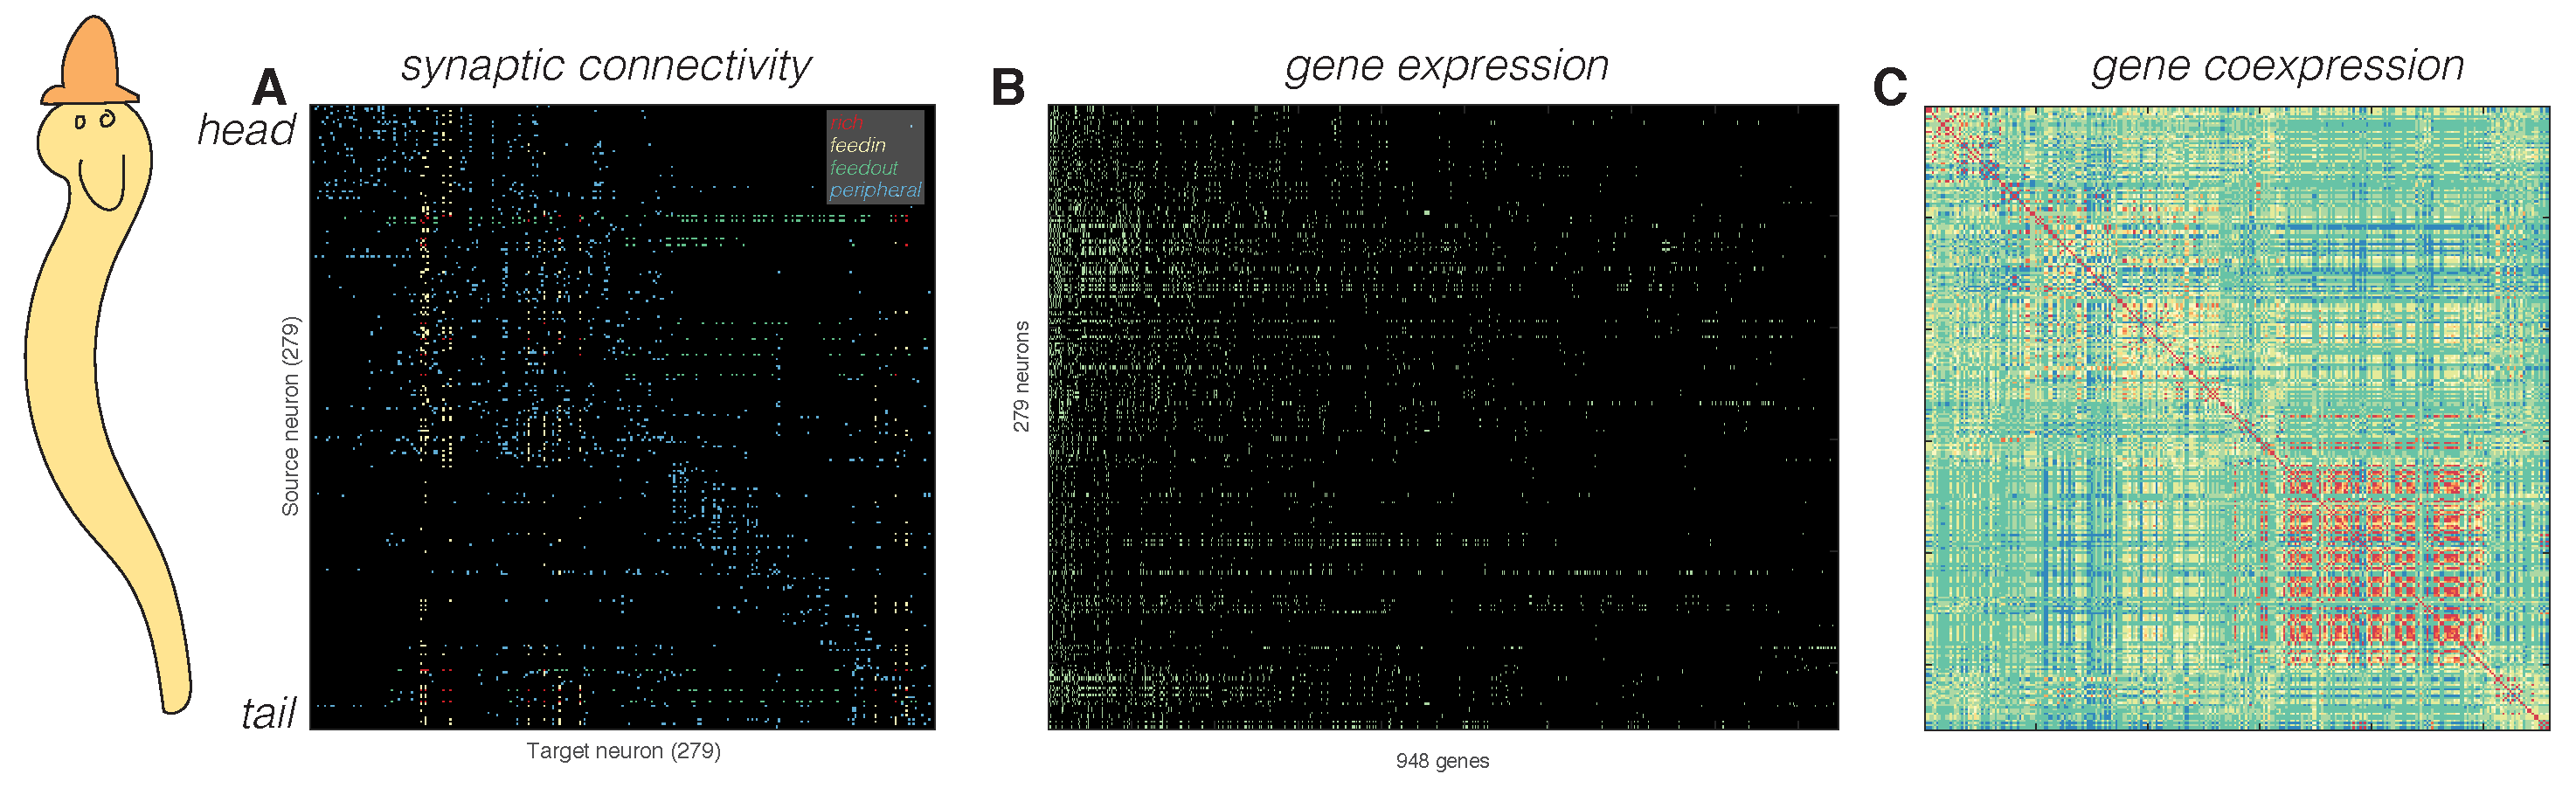
\includegraphics[width=1\textwidth]{schematic.pdf}
 \caption{\textbf{Schematic representation of the data used in this study.}
All plots show neurons (rows) ordered by their longitudinal position, from the top of the head (upper) to bottom of the tail (lower).
Schematic representation of the \textit{C. elegans} worm nervous system is shown on the left (scale of the animal is not preserved).
 \textbf{A} 2\,990 directed connections between 279 neurons from neuron $i$ (row) to neuron $j$ (column).
Connections are colored according to how they connect hubs ($k > 44$) and non-hubs ($k \leq 44$), as `rich' (hub $\rightarrow$ hub), `feed-in' (nonhub $\rightarrow$ hub), `feed-out' (nonhub $\rightarrow$ hub), and `peripheral' (nonhub $\rightarrow$ nonhub).
  \textbf{B} Binary gene expression indicated as a green dot when a gene (column) is expressed in a neuron (row).
% The 948 genes (columns) are expressed in each of the a neuron that are expressed in at least one neuron.
 \textbf{C} Gene coexpression matrix, computed for all pairs of neurons as the mean square contingency coefficient, $r_\phi$.
[[TODO: Would be nice to put neuronal metadata on the edge (if clear enough to read) -- could perhaps remove the coexpression plot?]]
[[TODO: Add information about and permission for the head-tail diagram.]]
[[TODO: Add labels about head/tail because the data don't actually follow the spatial scale shown on the left]]WHY SHOW the picture of the worm then?
[[TODO: Check gene coexpression plot is correct ordering]] IT IS CORRECT
}
\label{fig:SchematicRepresentation}
\end{figure}
% ------------------------------------------------------------------------------


\subsection*{Hub connectivity in the C. elegans connectome}

Recent work has shown that many aspects of connectome organization can be partially accounted for by geometric effects, in particular, a decreasing probability of connectivity between neural elements with increasing anatomical distance \cite{Henderson:2014fg, Roberts2016, Horvat:2016ia}.
Unlike network analyses of mammalian brains, where all neurons are confined to a spatially contiguous organ, neurons of the \emph{C. elegans} nervous system are distributed throughout the entire organism, forming a dense cluster of 147 neurons in the head (all within 130\,$\mu m$), 105 sparser, mostly motor neurons (75\%) in the body (spanning 1.02\,mm), and a relatively dense cluster of 27 neurons in the tail (all within 90\,$\mu$m of each other), see Fig.~\ref{fig:neuronsSpace} for a plot of all neurons in space.
The connection probability for pairs of neurons decays sharply as a function of the physical distance between them, excluding connections between the body and head, and between the body and tail, cf. Figs.~\ref{fig:spatialEffectsMain}A,B), mirroring recent results of mesoscale mammalian brains, in mouse \cite{Goulas:2016hr, Fulcher:2016ck}, and rodents and primates \cite{Horvat:2016ia}.

% ------------------------------------------------------------------------------
% <<plotSpatialEffectsMain.m>>
% ------------------------------------------------------------------------------
\begin{figure}[h]
  \centering
    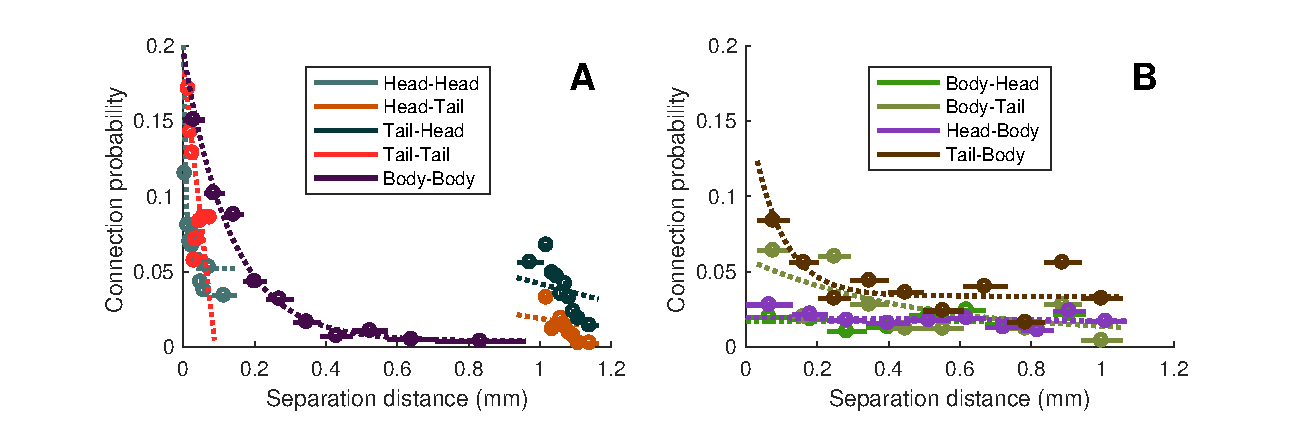
\includegraphics[width=\textwidth]{connectionProbability.eps}
  \caption{
\textbf{Connection probability decreases with separation distance within and between the head and tail, and within the body.}
The \emph{connection probability} for a pair of neurons as a function of their separation distance, estimated in 10 equiprobable distance bins, demonstrating a decrease for connections within the head (aqua), connections from head$\rightarrow$tail (brown) and from tail$\rightarrow$head (stone blue), connections within the tail (red), and connections within the body (dark purple).
Connection probability in each distance bin is shown as a circle (bin centers) and a horizontal line (bin extent).
Exponential fits, $f(x) = a\exp(-bx)+c$ (some of which appear linear across the range of the data), are shown as dotted lines.
\textbf{B}
Plots as in \textbf{A}, but for connection classes between the body and head/tail: from body$\rightarrow$head (forest green), from body$\rightarrow$tail (dirt green), connections from head $\rightarrow$ body (purple), and from tail$\rightarrow$body (dark brown).
Apart from a small effect at short range for tail$\rightarrow$body connections, these connection classes show minimal distance dependence.
% A decreasing relationship is evident up to a separation distance of approximately 0.2\,mm (driven by tail-tail and head-head connections), with a longer-range decrease up to $\approx$0.5\,mm due to body-body connections.
% The increase at large distances ($\approx 1$\,mm) is due to head-tail connections, which also show a decay with distance, from $\approx 1$\,mm through to $\approx$1.2\,mm.
% connections between body and head and body and tail showed no clear distance dependence.}
  }
  \label{fig:spatialEffectsMain}
\end{figure}


%%
%% INTRODUCE RICH CLUB  hene and focus on the difference between rich/feeder/peripheral links below
% [[TODO: Shorten section, focusing on reproducing Towlson]]
% \paragraph{Rich club organization of the connectome}

% <<hubs>>
% First, we analyze the topological properties of the \emph{C. elegans} connectome, represented here as a directed, binary connectivity matrix of 2194 chemical connections between 279 non-pharingeal neurons (1961 pairs of connected neurons) \cite{Varshney2011}, focusing particularly on hub connectivity.
The degree distribution of the \emph{C. elegans} synaptic connectome is shown in Fig.~\ref{fig:topology_rich}A, where neurons are distinguished by type: 68 sensory neurons, 85 interneurons, 108 motor neurons, and 18 multimodal neurons.
Despite using a directed connectome (rather than a symmetrized version in Towlson et al.~\cite{Towlson:2013gf}), we see a positively-skewed degree distribution containing an extended tail of high-degree interneurons that overlap almost completely with the list of Towlson et al.~\cite{Towlson:2013gf} (the list of hub neurons for the connectome used here is in Table~\ref{tab:HubList}).
These high-degree interneurons form the anatomical substrate for behaviors like coordinated locomotion and foraging \cite{tsalik2003}.
% connectivity between interneurons in the rich club provides the anatomical basis for vital neuronal computation of behaviours, such as coordinated locomotion and foraging36,37. Forward and backward movements, for example, are generated in two functionally separate subsets of neurons in this core, potentially coordinated through reciprocal inhibi- tion37,44. Moreover, a study recently demonstrated that random search behaviour in the worm can be approx- imated by a connectome-based stochastic model of this circuit4

% Here we confirm the high connectivity, centrality and wiring cost of hub connections in the C elegans connectome, as previoulsy shown by Towlson et al () and as also found in the macaue (Harriger) and human (van den Huevel-PNAS) brains.
% We show RC organization... and show hubs are interneurions...
% We show cost and centrality (may be worth including a curve for betweenness)


% ------------------------------------------------------------------------------
% <<TopologyFigures.m>>
% ------------------------------------------------------------------------------
\begin{figure}[h]
   \centering
    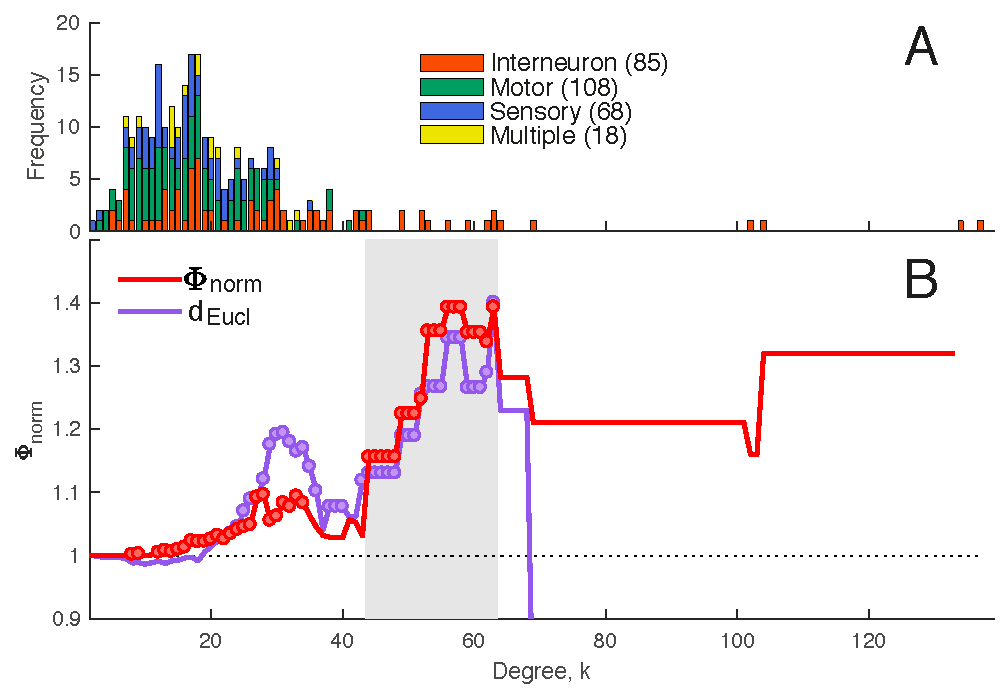
\includegraphics[width=0.9\textwidth]{topologicalRCall.pdf}
    % 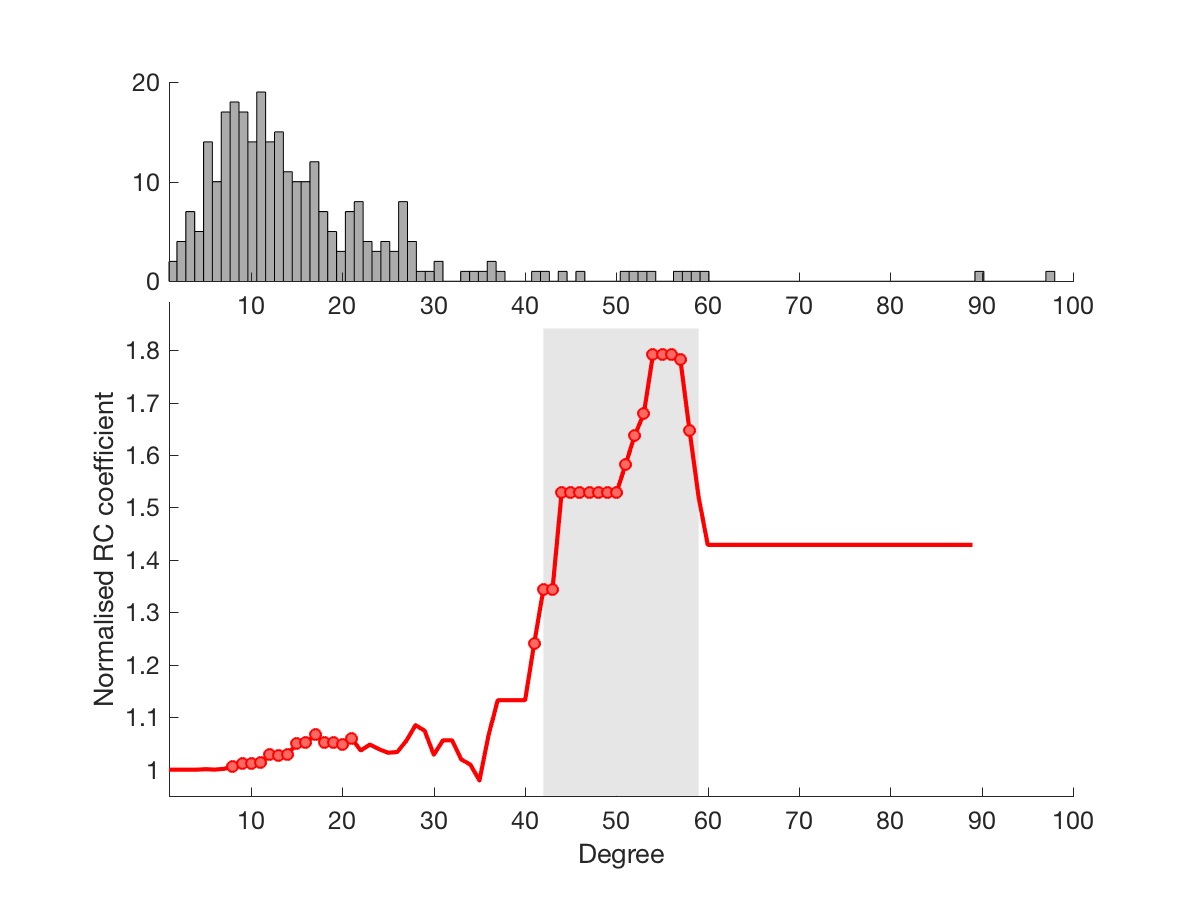
\includegraphics[width=0.7\textwidth]{RCcurve.eps}
 \caption{\textbf{Rich-club organization of the connectome}.
% A: Topological rich-club. B: Mixed rich-club. C: Weighted rich-club.
\textbf{A} Degree distribution of the binary chemical connectome, where neurons are labeled according to four categories:
(i) interneuron (85 neurons, orange),
(ii) sensory (68 neurons, blue),
(iii) motor (108 neurons, green), or
(iv) multiple assignments (18 neurons, yellow).
An extended tail containing neurons with relatively high degree is evident in the distribution.
Most of these neurons are interneurons.
\textbf{B}
Normalized rich club coefficient, $\Phi_\mathrm{norm}$ (red), as a function of the degree, $k$, at which hubs are defined (as neurons with degree $>k$).
Also shown is the mean Euclidean separation distance (purple) between connected hub regions (across degree thresholds, $k$).
$\Phi_\mathrm{norm} > 1$ indicates that hubs are more densely interconnected among each other than expected by chance, with red circles indicate values of $\Phi_\mathrm{norm}$ that are significantly higher than an ensemble of 1\,000 degree-matched null networks ($P < 0.05$).
Purple circles indicate where the Euclidean distance between connected pairs of hubs is significantly greater than the Euclidean distance for all other pairs of connected regions (Welch's $t$-test, $P < 0.05$).
[[TODO: Also suggest replacing red with one of these, since red is used in coexpression plot to represent something different]]
[[TODO: Add right-side vertical-axis to give units for distance]]
}
 \label{fig:topology_rich}
 \end{figure}
% ------------------------------------------------------------------------------


% ------------------------------------------------------------------------------
% <<rich-club organization>>
% ------------------------------------------------------------------------------
We quantified the extend to which hubs are densely interconnected by computing the normalized rich-club coefficient, $\Phi_\mathrm{norm}$, with $\Phi_\mathrm{norm} > 1$ indicating rich-club organization of the network.
Rich-club organization of the \emph{C. elegans} connectome was first demonstrated by Towlson et al. \cite{Towlson:2013gf}, who included both synaptic connections as well as gap junctions and symmetrized the directed synaptic connectivity (despite only 233 out of 1\,961 pairs of connected neurons being reciprocally connected), whereas here we retain the directed architecture of the connectome.
%and exclude gap junctions (to prevent them contributing to a different gene expression signature).
Accordingly, we define rich-club organization in relation to the sum of incoming and outgoing projections to a given neuron (total degree, $k$).
% Specifically, we find that
% Adj = GiveMeAdj(C,'zeroBinary','ch');
% reciprocal: sum(sum(Adj & Adj'))/2 = 233
% unidirectional: sum(sum(Adj & ~Adj')) = 1728
% either: sum(sum(Adj | Adj'))/2 = 1961
Figure~\ref{fig:topology_rich}B shows the variation of the normalized rich-club coefficient, $\Phi_\mathrm{norm}$, across degree thresholds, $k$, at which hubs are defined (as neurons with degree $>k$), with red circles indicating a significant increase in link density among hubs relatively to 1\,000 degree-preserving nulls (permutation test, $P < 0.05$) [[check whether randmio\_dir only preserves degree: AA - degree distributions in binary, out-strength (but not in-strength) in weighted]].
The plot reveals rich-club organization at the upper tail of the degree distribution, particularly for thresholds $44 < k < 63$, referred to here as the `topological rich-club regime', and shaded gray in Fig.~\ref{fig:topology_rich}B.
This result is similar to prior analysis of Towlson et al. \cite{Towlson:2013gf}, despite using a directed synaptic connectome here rather than a symmetrized connectome including gap junctions.
We also repeated the analysis with two different definitions of weighted rich-clubs \cite{Opsahl2008}, which also yielded similar results (shown in Fig.~\ref{fig:S_weightedRC}).
% This indicates that when nodes are defined as hubs (degree $>\textit{k}$) in this range, they are more densely interconnected than expected by chance.
We use a hub definition in this work of $k > 44$, which corresponds to the lowest degree threshold at which the network displays significant rich-club organization (permutation test, $P < 0.05$).
 % of the analyses presented below examine how different topological and genomic properties vary as a function of the hub threshold, $k$, but for analyses requiring a fixed hub definition, we define hubs as the 13 neurons with
The distribution of hubs and hub-hub connections in two-dimensional space is shown in Fig.~\ref{fig:neuronsSpace}.


% Rich club in the chemical synapse network consists of 13 high degree neurons with degree $42 \leq k \leq 98$.
% When comparing the normalized rich club coefficient $\Phi_\mathrm{norm}$ as a function of degree in both cases we notice that $\Phi_\mathrm{norm}$ reaches slightly higher values for a directed chemical synapse connectome in the topological rich-club regime ($\Phi_\mathrm{normMAX} = 1.8$), while an increase in the symmetrized connectome is not so sharp ($\Phi_\mathrm{normMAX} = 1.4$) meaning that the  rich club effect might me slightly more pronounced in a directed version of a synaptic connectome.

% ------------------------------------------------------------------------------
% <<distance, geometric effects>>
% ------------------------------------------------------------------------------
% <<cf. NeuronTypeStats.m to run these numbers>>
In Fig.~\ref{fig:topology_rich}B, we plot the mean distance between all pairs of connected hubs at each degree threshold, $k$.
Consistent with the analysis of Towlson et al. \cite{Towlson:2013gf}, we find an increase in mean hub-hub connection distance with $k$, through to the extent of the topological rich-club regime.
This result can be attributed to a relative increase in long-distance hub-hub connections between the head and tail (Fig.~\ref{fig:S_connectionProportion}).
The high connection density and long mean anatomical distance of hub-hub pairs counters the general trend in the \emph{C. elegans} connectome, where the probability of connectivity between two neurons decays sharply as a function their separation distance.
Taken together, our results demonstrate that hub-hub connections in \emph{C. elegans} are dense and extend over significantly longer distances than other types of connections in the synaptic network of the nematode nervous system, consistent with the rich club forming a central yet costly backbone for neuronal communication \cite{vandenHeuvel:2012kh}.

% In connectomes across species and scales, degree is distributed unequally, with a small number of highly connected brain regions, known as hubs \cite{Sporns:2007ea}, that are themselves more densely connected between themselves, forming a so-called `rich club' \cite{deReus:2013cy, ZamoraLopez:2010hy, Shih:2015cu, vandenHeuvel:2012kh, vandenHeuvel:2011he}.
% The same is true in the C. elegans neuronal nervous system, analyzed in the past as an undirected binary connectome including both chemical and electrical synapses \cite{Towlson:2013gf}, which exhibits highly connected, and densely interconnected hub neurons.

% ------------------------------------------------------------------------------
% \paragraph*{S5 Fig.}
% {\bf Spatial distribution of rich links, and neuron types across the C. elegans nervous system. }
\begin{figure}[h]
\centering
    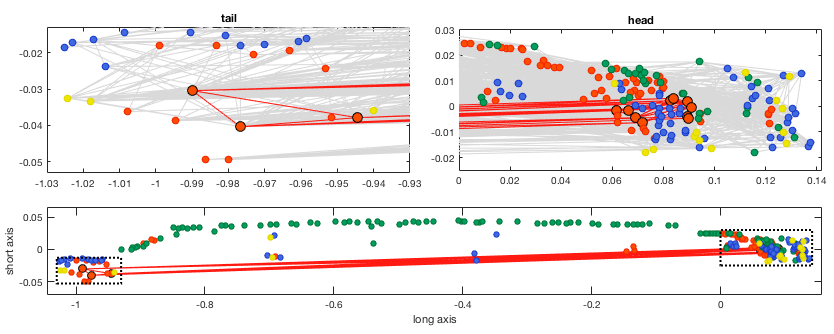
\includegraphics[width=1\textwidth]{SpatialPlot.png}
\caption{
\textbf{Spatial distribution of neurons and hub-hub links across the C. elegans nervous system}.
Neurons are positioned along the Posterior (P)-Anterior (A) (horizontal), and Ventral (V)--Dorsal (D) (vertical) axes.
% Definitions of posterior/anterior/ventral/dorsal from Varier.
Neurons are colored by type:
(i) interneuron (85 neurons, orange),
(ii) sensory (68 neurons, blue),
(iii) motor (108 neurons, green), or
(iv) multiple assignments (18 neurons, yellow).
Hub-hub links are shown, and zoom-in plots of head and tail are shown as dotted rectangles in the lower plot.
In each plot, axes are to scale.
\label{fig:neuronsSpace}
}
\end{figure}
% ------------------------------------------------------------------------------

%%
\subsection*{Coexpression and connectivity}

% ---connectivity/coexpression---
Having characterized the topological and geometric properties of rich-club connectivity in \emph{C. elegans}, we next investigate how axonal connectivity properties relate to gene expression patterns.
Being a pairwise analysis, we compare pairwise synaptic connectivity to pairwise similarity in gene expression, measured by the mean square contingency coefficient, $r_\phi$ (see \emph{Methods}).
% , to define gene coexpression, and excluding coexpression values between homologous left/right neuron pairs, see Methods).

First we investigate whether gene coexpression relates to synaptic connectivity by comparing the distribution of $r_\phi$ computed for all connected pairs of neurons, and for all unconnected pairs of neurons, shown in Fig.~\ref{fig:coExp}A.
We find that connected pairs of neurons have more similar expression profiles than unconnected pairs (Wilcoxon rank-sum test, $P < 10^{-78}$), mirroring results in the mesoscale mouse connectome \cite{Fulcher:2016ck}.
Moreover, we also demonstrate increased coexpression between neuron pairs connected via gap junctions compared to neurons connected via chemical synapses (Wilcoxon rank-sum test, $P < 10^{-22}$).
Afterwards, we separated connections into three distinct categories: electrical, chemical reciprocal ($X \leftrightarrow Y$) and chemical unidirectional ($X \rightarrow Y$), however, unlike in the mouse brain, we found no differences in gene coexpression, $r_\phi$, between chemical unidirectional and reciprocal connections (see Fig.~\ref{fig:S_RFPdistributions}).

% ------------------------------------------------------------------------------
% <<coexpConnUncon.m>>
% <<RichClub.m>>
% ------------------------------------------------------------------------------
 \begin{figure}[h]
 \centering
    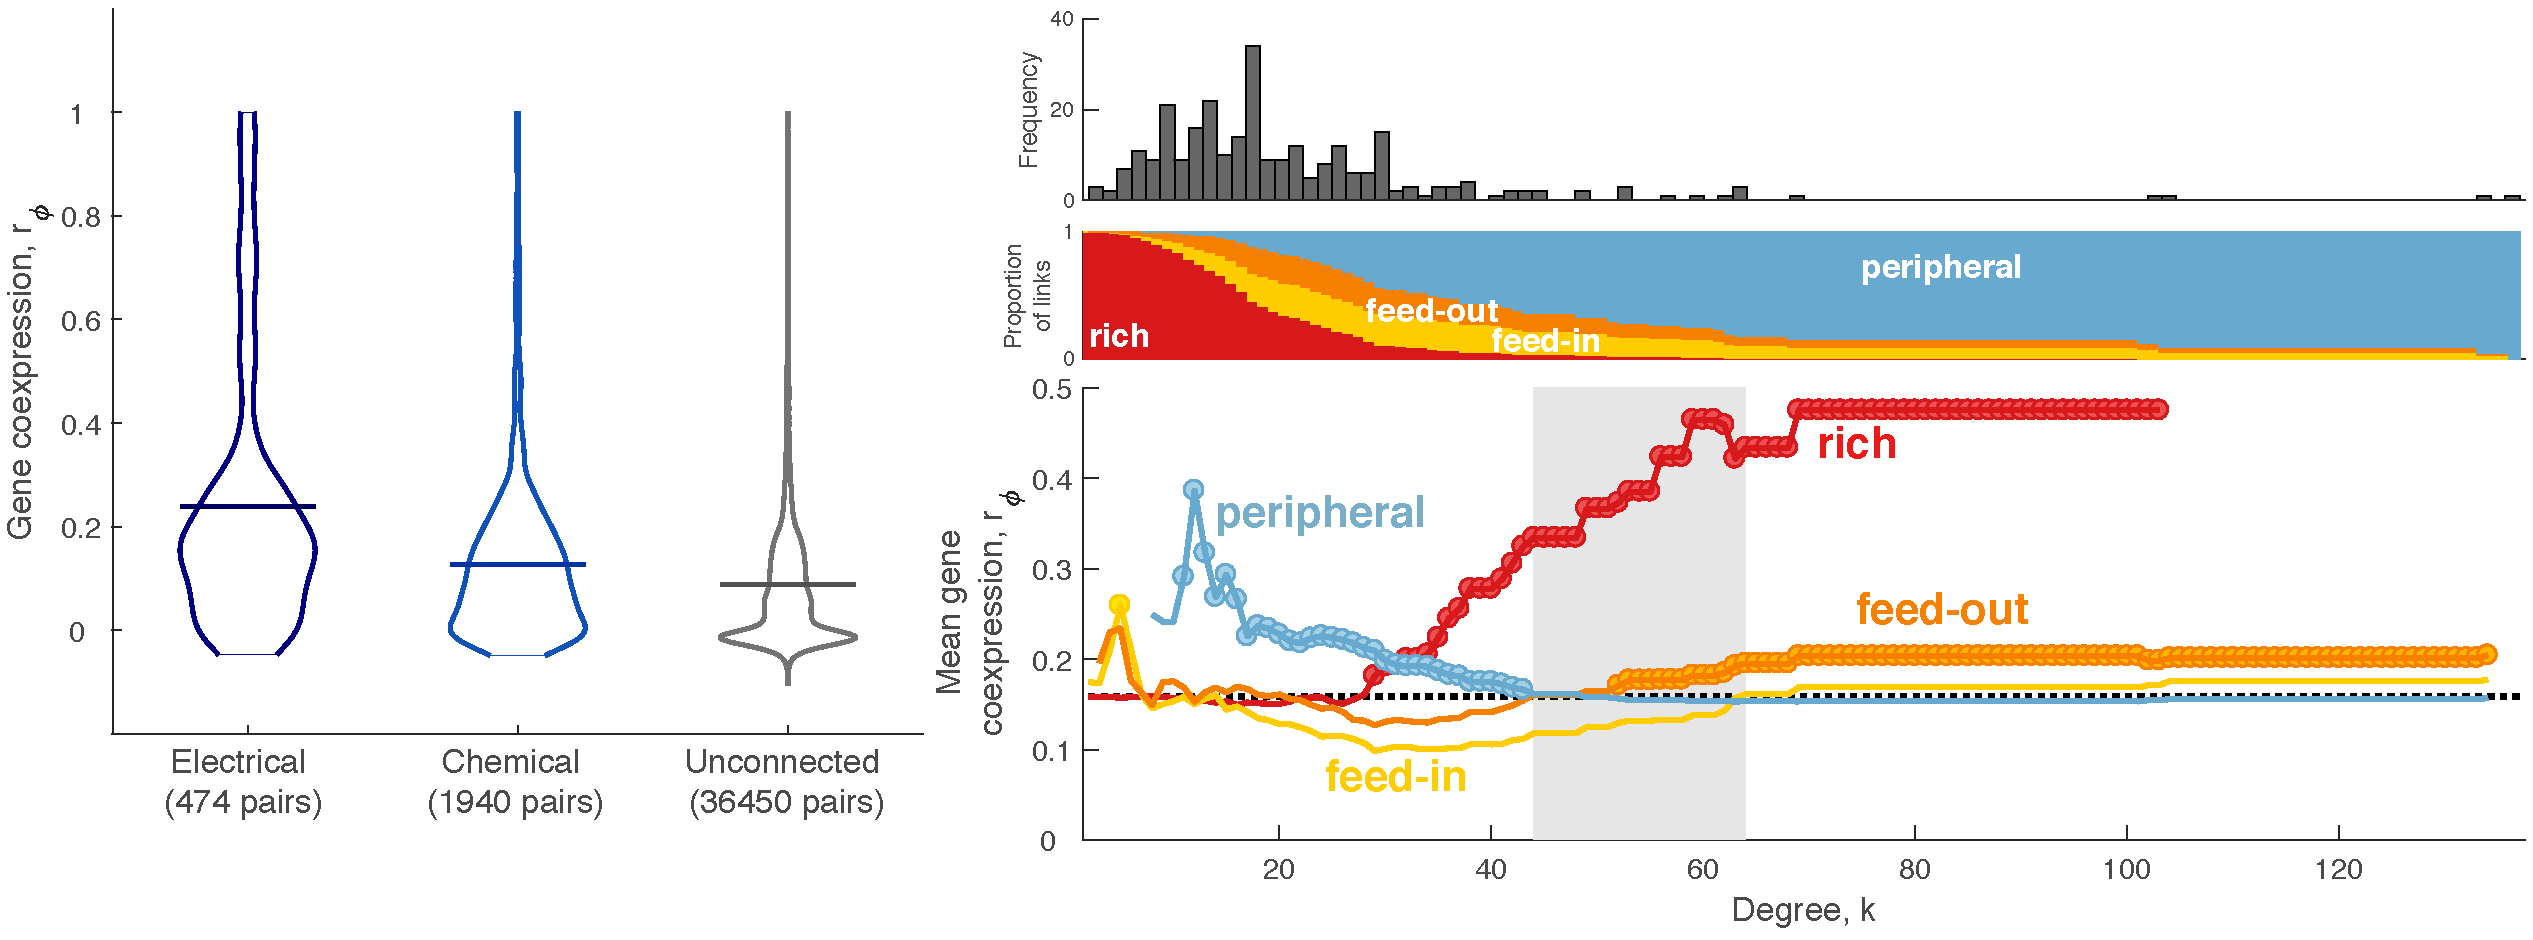
\includegraphics[width=1\textwidth]{MeanCoexpressionALL.pdf}
 \caption{{\bf Gene coexpression varies as a function of connectedness and connection type, with the highest coexpression for connections involving hubs.}
\textbf{A} Distribution of transcriptional similarity between electrically connected, chemically connected and unconnected pairs of neurons as a violin plot, with the mean of each distribution represented by a horizontal line.
Note that connections between bilateral pairs of neurons display high transcriptional similarity and are excluded from this analysis, leaving 474 electrically (514-40), 1\,940 connected pairs (1\,961 - 21) and 36\,450 unconnected pairs (36\,494 - 44).
The categories of electrically and chemically connected neuron pairs are not mutually exclusive with 175 pairs of neurons connected via both types of connections. 
Coexpression, $r_\phi$, is increased in connected compared to unconnected pairs of neurons ($P < 10^{-78}$, Wilcoxon rank sum test).
Coexpression, $r_\phi$, is increased in neuron pairs connected via electrical synapses compared to pairs connected via chemical synapses ($P < 10^{-22}$, Wilcoxon rank sum test).
\textbf{B}
\emph{Top}: Degree distribution, $k$, of the \emph{C. elegans} synaptic connectome.
\emph{Middle}: proportion of connections that are `rich' (hub$\rightarrow$hub, red), `feed-in' (nonhub$\rightarrow$hub, yellow), `feed-out' (hub$\rightarrow$nonhub, orange), and `peripheral' (nonhub$\rightarrow$nonhub, blue) as a function of the degree threshold, $k$, used to define hubs.
Note that at high $k$, most neurons are labeled as nonhubs, and hence the vast majority of connections are `peripheral'.
\emph{Bottom}: Mean gene coexpression, $r_\phi$, for each connection type as a function of $k$.
The mean coexpression across all network links is shown as a dotted black line; the topological rich-club regime (determined from the network topology, cf. Fig.~\ref{fig:topology_rich}) is shaded gray.
Circles indicate a statistically significant increase in gene coexpression in a given link type relative to the rest of the network (one-sided Welch's $t$-test; $P < 0.05$).
[[TODO: fonts are small, and inconsistent sizes between subplots.
I think we should crop the curves when there are fewer than X connections remaining -- in this case it's a bit ridiculous to show that constant feed-out/feed-in/peripheral coexpression when there are only two neurons
left as hubs]]
[[TODO: Font size inconsistent in B]]
}
 \label{fig:coExp}
\end{figure}
% ------------------------------------------------------------------------------

% ---HUB coexpression---
We next investigated whether coexpression varied between different types of connections, focusing particularly on the role of densely interconnected hub neurons.
% characterized above, hypothesizing an increase in connections involving hubs, with hub-hub connections displaying the most similar gene expression patterns \cite{Fulcher:2016ck}.
% Given the importance of hub neurons across species [[Ref]], and previous results in the mesoscale mouse connectome \cite{Fulcher:2016ck},
For a given hub threshold, $k$, we first labeled each neuron as either a `hub' (nodes with degree $> k$) or a `nonhub' (degree $\leq k$), and then labeled each connection as either `rich' (hub $\rightarrow$ hub), `feed-in' (nonhub $\rightarrow$ hub), `feed-out' (hub $\rightarrow$ nonhub), or `peripheral' (nonhub $\rightarrow$ nonhub).
% [[TODO: Establish whether we're computing pairs of hubs (e.g., for `rich'), or for every connection between any pair of hubs -- i.e., do reciprocal connections contribute twice to the distribution at each $k$? AA: as in original mouse analysis -- all connections, but we take mean, so the mean doesn't change in either way]]
The mean coexpression for each of these four connection types is plotted in Fig.~\ref{fig:coExp}B, with circles indicating statistically significant increases of a given connection type (relative to all other connections, $P < 0.05$, Welch's $t$-test).
Gene coexpression in rich connections increases with degree, through the topological rich-club regime where hubs are densely interconnected (shaded gray in Fig.~\ref{fig:coExp}B).
Feed-out connections exhibit some increased gene coexpression in the topological rich-club regime, while feed-in and peripheral connections show the lowest levels of coexpression.
Full distributions of coexpression at a hub threshold of $k > 44$ are plotted in Fig.~\ref{fig:S_RFPdistributions}.

These results, using partial binary annotations of gene expression across just 948 genes in a microscale neuronal connectome, are consistent with a prior analysis of the expression of over 17\,000 genes across 213 regions of the mesoscale mouse connectome.
Specifically, both connectomes display:
(i) increased coexpression in connected pairs of nodes;
(ii) the highest coexpression in rich connections;
(iii) intermediate coexpression in feeder connections; and
(iv) lowest coexpression in peripheral connections.

\subsection*{Potential drivers of elevated coexpression in pairs of hubs}
The hubs of the mouse connectome are broadly distributed across anatomical divisions \cite{Fulcher:2016ck}, the 16 hub neurons in \emph{C. elegans} ($k > 44$) are all interneurons, are all born before hatching, are mostly cholinergic (13/16), and are mostly contained within a single network module.
% and concentrated in the head (10/13),
% \cite{Varier2011}, \cite{Pereira:2015er}
% Having demonstrated that gene coexpression is elevated for connected regions, and particularly for connected pairs of hubs,
We thus investigated whether the similarity of gene expression profiles between hubs was specific to their high levels of connectivity, or whether it could instead be explained by similarity in one or more of these characteristics.
% We thus investigated whether any of these types of homogeneities amongst hub neurons could contribute to our finding of increased gene coexpression, $r_\phi$.
% , namely modular organization, lineage similarity, or neurotransmitter type, could explain our results.

% \paragraph{Distance}).
% Implementing the same methods as previously used in gene coexpression analysis at each degree threshold for each link type (rich, feeder, peripheral) we calculated the mean connection distance.
% Connection distance increased with increasing degree for both rich and feeder links while peripheral connections demonstrated no increase through the whole range of thresholds (Fig.~\ref{Distance}).
% Given this result, it is safe to say that increased coexpression for hub-related links is not determined by lower connection distance between them as the contrary is shown to be true.

%\begin{figure}[!h]
%\centering
 %   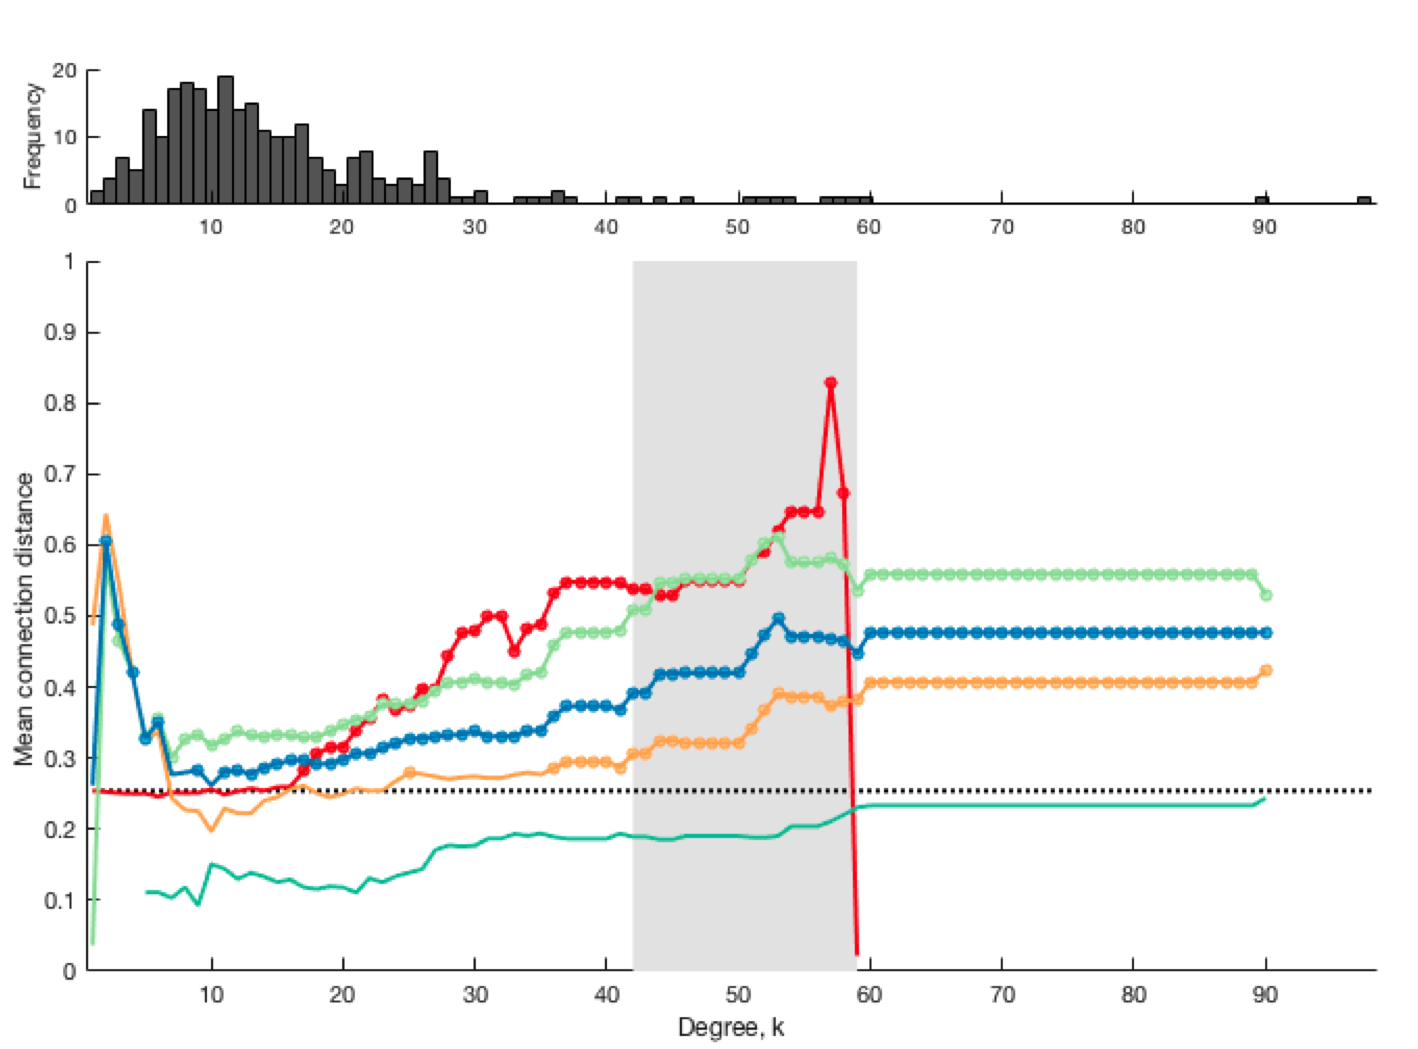
\includegraphics[width=0.7\textwidth]{distance_k}
 %\caption{{\bf Connection distance as a function of degree}}
 %\label{Distance}
 %\end{figure}

\paragraph{Neuron type}
Neurons in \emph{C. elegans} are annotated to the following functional categories: sensory neurons, motor neurons, and interneurons (with eighteen multifunctional neurons annotated to two categories).
All hubs ($k > 44$) are interneurons (cf. Fig.~\ref{fig:topology_rich}A), matching the finding of Towlson et al.~\cite{Towlson:2013gf}.
To determine whether the increase in gene coexpression in rich connections was specific to one of these neuron types, we split our coexpression analysis into connections involving: (i) interneurons, (ii) sensory neurons, and (iii) motor neurons.
In Fig.~\ref{fig:interneuron_dep}A, we plot the mean coexpression for hub-hub connections (as a function of $k$) separately for (i) connections involving interneurons, (ii) connections involving sensory neurons, and (iii) connections involving motor neurons.
For the curve labeled `sensory' neurons, for example, each point is $\langle r_\phi \rangle$, computed across connections involving sensory neurons (i.e., at least one neuron of a connected pair is a sensory neuron), for which both neurons have degree $>k$.
% Thus, the three categories are not mutually exclusive; for example, the `interneuron' class includes connections between an interneuron and any other neuron.
The plot shows that the increase in hub-hub gene coexpression with degree is driven by interneurons while connections involving motor neurons show only a marginal increase with degree and connections involving sensory neurons, even show a slight decrease in coexpression as a function of $k$.
% , which are unique in their increasing average coexpression with increasing degree
% Thus, interneurons drive the gene coexpression relationship with degree, $k$,

% ------------------------------------------------------------------------------
% <<plot_neuronType.m>>
% ------------------------------------------------------------------------------
\begin{figure}[h]
\centering
   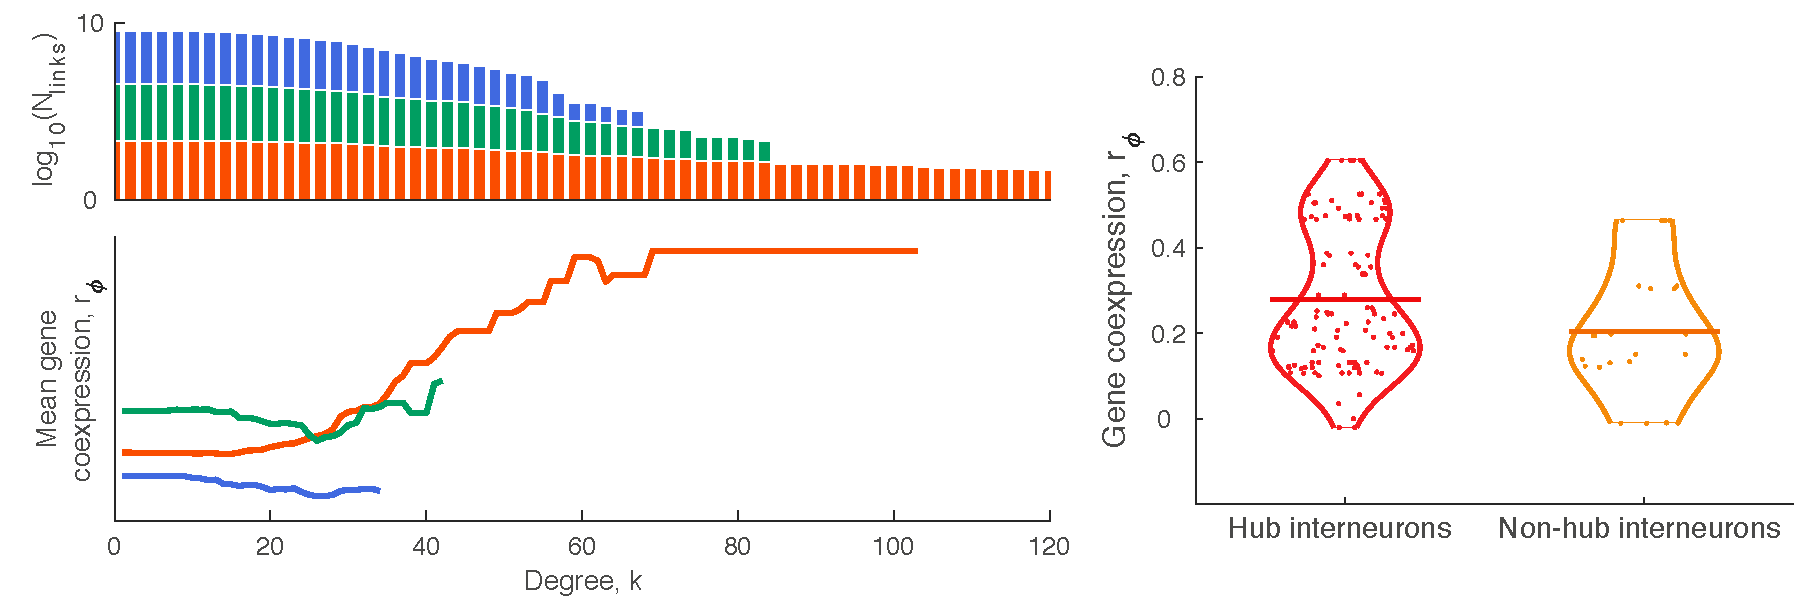
\includegraphics[width=1\textwidth]{DegreeTypeALL.pdf}
 \caption{
\textbf{The increase in coexpression with degree is specific to high-degree interneurons, and hub interneurons have higher coexpression than nonhub interneurons.}
\textbf{A} \emph{Top}: The number of connections involving interneurons (orange), sensory neurons (blue), and motor neurons (green) across degree threshold, $k$ represented as $log_{10}$(number of links).
\emph{Bottom}: Average gene coexpression as a function of degree for connections involving different types of neurons.
\textbf{B} Coexpression distributions for all pairs of hub interneurons (red) and all pairs of non-hub interneurons (gray) ($P = 0.047$, Wilcoxon rank sum test).
%[[TODO: Remove big circles from A? Confusing to keep balls because they look like they correspond to statistical significance, as above]]
%[[TODO: see if B looks good with data points]]
}
 \label{fig:interneuron_dep}
\end{figure}

[[MAKE LESS VAGUE]] [[NEED A STRONGER ARGUMENT FOR SELECTING THOSE SPECIFIC INTERNEURONS]]:\\

% Having found that interneurons drive the gene coexpression relationship with degree, $k$,
We next sought to verify whether hubs show a unique transcriptional signature amongst interneurons.
Given that hubs exhibit significantly higher coexpression compared to other interneurons ($P < 10^{-34}$, Wilcoxon rank sum test, data not shown), we aimed to select a subset of interneurons that would most closely resemble hub interneurons in terms of anatomical properties in order to verify if even among similar interneurons hubs show a specific gene expression pattern.
Therefore, we choose a subset of interneurons that originate and terminate in approximately the same locations as hub interneurons, however are not required to have similar connectivity pattern.
We compared gene coexpression between all pairs of hub interneurons ($\textit{k}>44$, $n=16$) and all pairs of nonhub interneurons (AVFL, AVFR, AVHL, AVHR, AVKL, AVKR, AVJL, AVJR, $n=8$) ignoring the presence of absence of connections between them in order to ensure that increase in coexpression for rich links is not determined by the fact that the majority of hub neurons belong to the same anatomical neuron type.
%To determine whether hub neurons of this anatomical type showed more similar expression patterns than nonhubs of the same type, we computed the gene coexpression, $r_\phi$, between all pairs of hub neurons and all pairs of non-hub neurons (ignoring their connectivity for this analysis).
As shown in Fig.~\ref{fig:interneuron_dep}B, pairs of hub interneurons exhibit significantly higher gene coexpression than pairs of nonhub interneurons ($P = 0.047$, Wilcoxon rank sum test).
Thus, the increase in coexpression amongst hub interneurons is not simply due to most hubs being interneurons as even amongst interneurons sharing same anatomical properties hub interneurons exhibit significantly increased coexpression.

\paragraph{Modular organization}
The \emph{C. elegans} synaptic nervous system has a modular organization, in which subsets of neurons show dense interconnectivity \cite{Kim2014, Pan:2010jt, Bassett2010}, or exhibit similar connectivity patterns to each other \cite{Achacoso:1992ay, Pavlovic2014}.
% , which can correspond to specific functional circuits
A common assumption is that connectome modules correspond to functionally specialized systems and it is therefore plausible that neurons belonging to the same module might exhibit similar gene expression patterns, as has been shown for macroscopic functional networks in the human brain \cite{Richiardi2015}.
Brain network hubs generally participate in multiple modules \cite{vandenHeuvel:2013ij, deReus:2014cz}, and their dense rich-club connectivity implies that they even form their own module that overlaps with other, more specialized systems \cite{Fornito:2015dq, deReus:2013cy, ZamoraLopez:2010hy}.
Here we sought to determine whether our finding of increased coexpression between pairs of hub neurons in the \emph{C. elegans} connectome can be explained by its modular organization.
% , driven by the characteristic gene expression of that module.

We used the Louvain community detection algorithm \cite{Blondel:2008do} to extract modules from the \emph{C. elegans} synaptic connectome using consensus clustering (see \textit{Methods}).
The four resulting modules are shown in Fig.~\ref{fig:OtherInfluences}A.
The majority of hub neurons belong to the module labeled in green.
This is a diverse module, containing sensory, motor, and interneurons and spanning neurons in the head, tail, and body (see other indicator columns to the left of Fig.~\ref{fig:OtherInfluences}A).
% In this analysis, hubs are mostly concentrated in a single module (purple in Fig.~\ref{fig:modules}), but are also distributed across three other modules.
% The algorithm detects three comparably sized modules (M1-M3), each containing diverse neuron types, as well as a smaller fourth module (M4), which contains 13 motor neurons.
% Of the 13 hubs with $k \geq 42$, the majority (11) were assigned to M3, which spanned the length of the worm body, as pictured in Fig.~\ref{fig:modules}.
% As evident from the column labels to the left of the matrix, the hub-concentrated module is diverse, containing neurons across the head, tail, and body, as well as sensory, motor, and interneurons (see labels on Fig.~\ref{fig:modules}A).
% This module is comprised primarily of motor neurons, consistent with evidence that control interneurons are directly responsible for forward and backward locomotion (command interneurons).
% 10 out of 11 hub neurons in this module are directly responsible for
% The main goal of this analysis was to compare coexpression within and between modules in order to examine if neurons assigned to the same module are more genetically similar than neurons in other modules.
% The expectation that gene coexpression, $r_\phi$, was increased within modules was not observed.
In contrast to our expectations, there was no significant difference in gene coexpression for connections within modules compared to those between modules ($p = 0.69$, Wilcoxon rank sum test), as shown in Fig.~\ref{fig:OtherInfluences}B.
% CoexpressionDistributionsModules(C,G,'intraInter',true,'consensus');
This result is not due to our use of the Louvain community detection algorithm, as we also found no differences using a previous nine-module partition of neurons derived from an Erd\"os-R\'enyi Mixture Model ($p = 0.68$, Wilcoxon rank sum test) \cite{Pavlovic2014}.
% CoexpressionDistributionsModules(C,G,'intraInter',true,'ERMM');
Focusing on pairs of neurons within the same module, we found that coexpression was higher for connected pairs of hubs than connected pairs of nonhubs, as shown in Fig.~\ref{fig:OtherInfluences}C ($p = 4.4\times 10^{-29}$, Wilcoxon rank sum test).
% CoexpressionDistributionsModules(C,G,'hubIntra',true,'consensus');
We also computed an empirical null distribution for the mean coexpression across random sets of 55 intramodular and two intermodular links by taking 1\,000 random samples from these two link types across the network, yielding a null $r_\phi$ of $0.13 \pm 0.02$, compared to the observed value of $0.51$ ($p < 10^{-16}$).
The increase in hub-hub coexpression is thus not driven by a general increase of coexpression for pairs of neurons within the same topological module.
% Coexpression within modules did not exceed coexpression between modules, demonstrating that neurons that belong to the same module do not share any particular genetic similarity.
% The increased coexpression in connected pairs of hubs in \emph{C. elegans} can therefore not be attributed to the modular organization of the connectome.
% despite most hubs being assigned to the same module.
% [[NOTE: maybe not worth characterizing modules, just say: coexpression within modules is not higher than coexpression between modules on one sentence and distributions? When hub neurons are excluded, M2 and M3 coexpression is higher than M1, but no difference between M2 and M3]])

% [[TODO: this section required more justification. Why would we expect modules to drive hub effect? why is looking at modules in this context interesting? Unclear what the nulls are and how they were generated.]]

% ------------------------------------------------------------------------------
% <<plot_modules.m, plot_birthTime.m, plot_lineage.m>>
% ------------------------------------------------------------------------------
\begin{figure}[!h]
\centering
    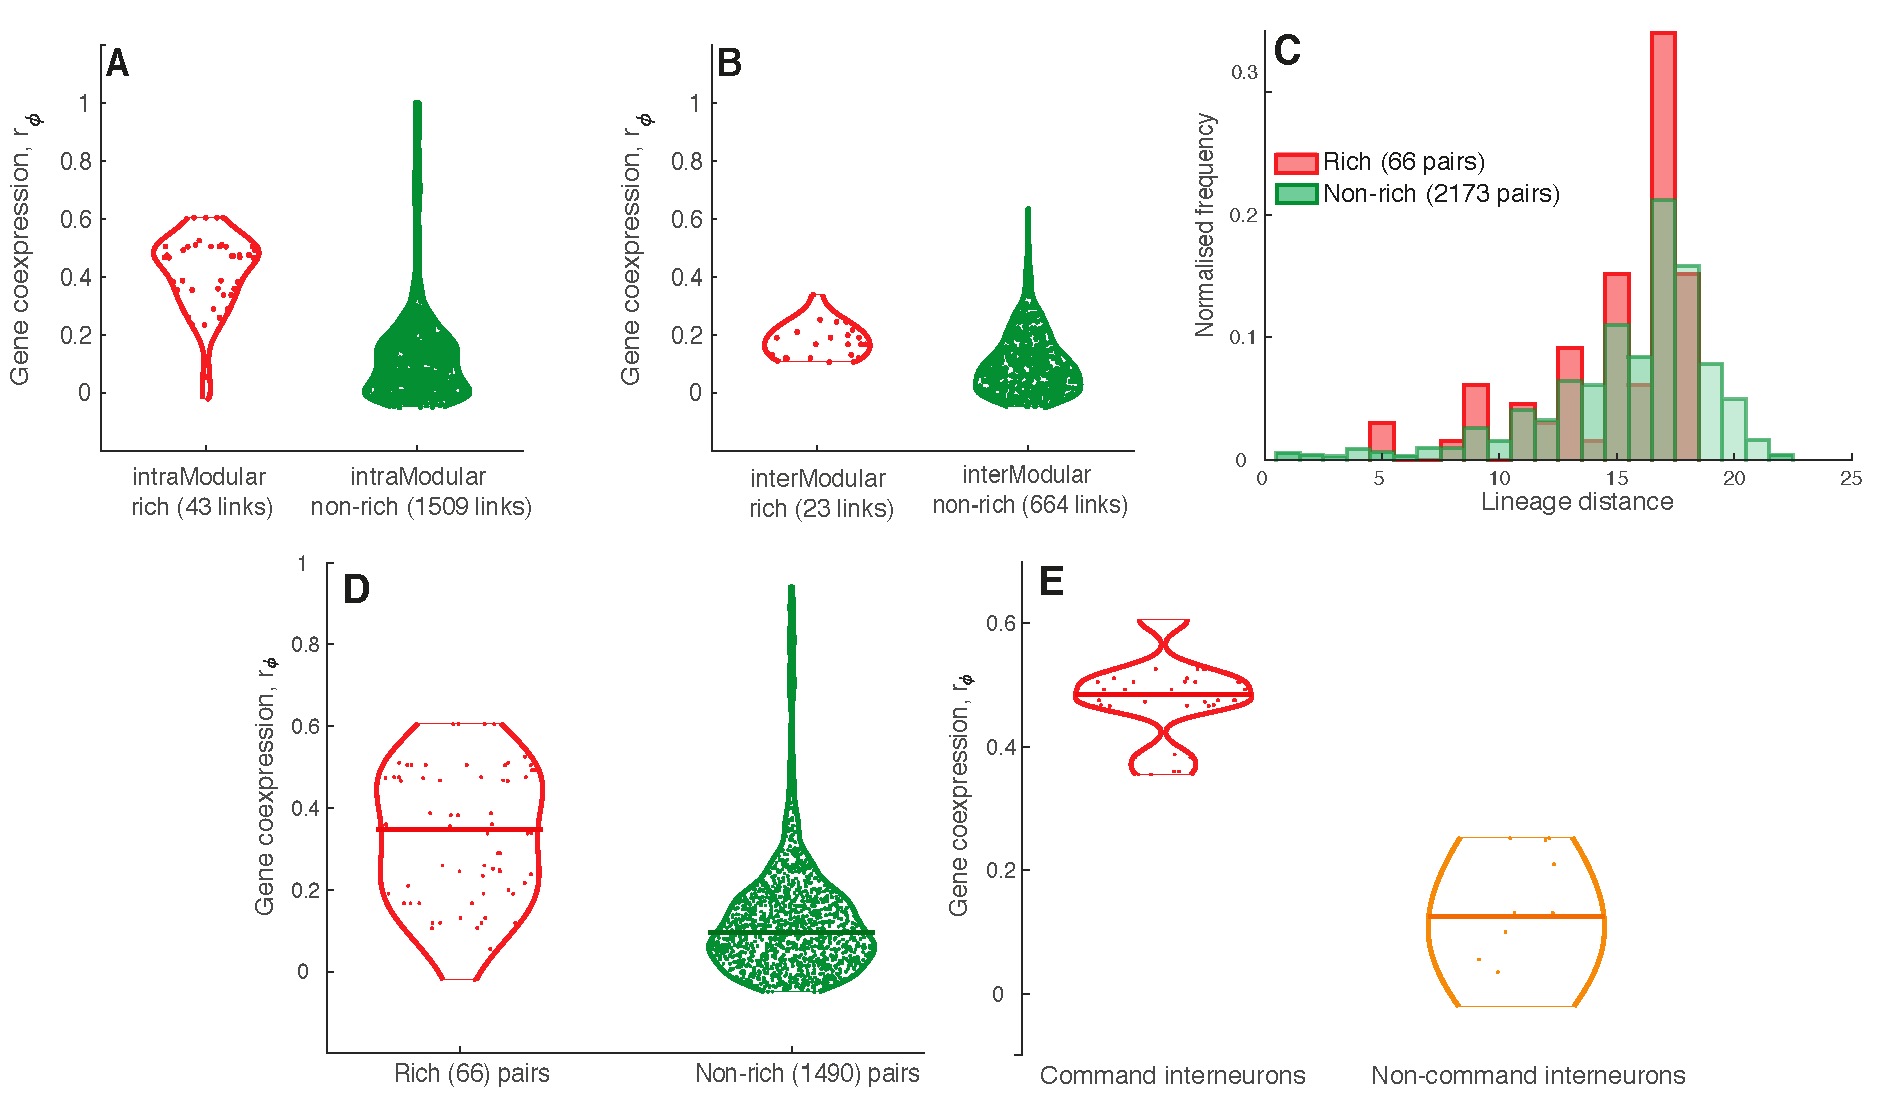
\includegraphics[width=1\textwidth]{extrasALL.pdf}
 \caption{
 \textbf{Increased coexpression of hub neurons is not driven by their membership of similar topological modules, similar birth times, or lineage distance.}
%\textbf{A: Connection distance}
%Top: Degree distribution.
%Bottom: Median lineage distance for rich, feeder, and peripheral connections as a function of \textit{k}, with the %median across all network links shown as a dashed black line and the topological rich club regime shaded grey.
%Circles indicate a statistically significant change in lineage distance in a given link type relative to the rest %of the network (Wilcoxon rank sum test; $P < 0.05$). \\
\textbf{A} Nematode connectivity matrix organized by topological module (white squares), with all connections labeled by type: rich (red), feed-in (yellow), feed-out (orange), and peripheral (blue).
Neuron indicators are shown to the left:
(i) module assignment,
(ii) neuron type (interneuron, orange; motor, green; sensory, blue; multimodal, yellow),
(iii) hub indicator (red for hubs), and
(iv) spatial position: head (gray), body (purple), tail (red).
\textbf{B} Distributions of gene coexpression, $r_\phi$, for intra-modular connections (black) and inter-modular connections (gray), shown as violin plots with the mean shown as a horizontal bar.
% The number of connections of each type is shown in parentheses.
\textbf{C} Distributions of gene coexpression, $r_\phi$, for intra-modular rich (red) and non-rich (blue) connections, shown as violin plots with the mean shown as a horizontal bar (Wilcoxon rank sum test, $p = 4.4\times 10^{-29}$).
% The number of connections of each type is shown in parentheses.
\textbf{D} Distributions of gene coexpression, $r_\phi$, for early born hubs (rich links, red) and non-hubs (non-rich links, blue) shown as violin plots with the mean shown as a horizontal bar. ($P < 10^{-28}$, Wilcoxon rank sum test).
\textbf{E} Distributions of lineage distance between rich links (red) and non-rich links (blue), plotted as histograms because lineage distance is discrete ($P = 0.91$, Wilcoxon rank sum test).
[[TODO: could add neurotransmitter type as a bar code in modules]]
[[TODO: change colors for distributions, fill distributions, e.g., intramodular and intermodular shouldn't use red (rich) and blue (non-rich) used in other plots. Blue is used for peripheral, so perhaps another color could be used for non-rich (green?)]]
%Composition of each module according to neuron type.
%Modular organisation of the connectome.
%Coexpression distributions within and between modules.
%\textbf{C: Lineage distance}
%Top: Degree distribution. Bottom: Mean lineage distance for rich, feeder, and peripheral connections as a function %of \textit{k}, with the median across all network links shown as a dashed black line and the topological rich club regime shaded grey.
%Circles indicate a statistically significant change in lineage distance in a given link type relative to the rest of the network (one-sided Welch’s t-test; $P < 0.05$) \\
%\textbf{D: Coexpression for different types of neurons. }
%Top: Median gene coexpression as a function of degree for connections involving different types of neurons.
%Bottom: The number of connections in each category for a range of degrees.
%Coexpression distributions for hub and non-hub interneurons.\\
}
 \label{fig:OtherInfluences}
\end{figure}


\paragraph{Birth time}
The genesis of neurons in the \emph{C. elegans} nervous system is separated into two distinct time periods: before hatching (birth time $<550$ min) and after hatching (birth time $>1200$ min), with no neurons formed during intermediate times \cite{Varier2011}.
Differences in birth times between pairs of neurons are dominated by the differences between these two temporal clusters of neuron birth.
% with an around 700min gap between them when no neurons are formed.
All \emph{C. elegans} hub neurons are born prior to hatching \cite{Varier2011, Towlson2013}.
It has been shown that neurons born at similar times may share similar properties including connectivity \cite{Schroter:2017eo}, we investigated whether the increase in coexpression between hub neurons is influenced by similarity in their birth time.
To test this hypothesis, we focused on 201 neurons (16 hub and 185 nonhub neurons) born prior to hatching (birth time $<550$\,min) to see whether connections between hub neurons displayed increased coexpression relative to other types of connections between neurons born during this early developmental phase.
As shown in Fig.~\ref{fig:OtherInfluences}D, even among early-born neurons, connections between hubs (rich) show significantly increased coexpression compared to all other connections (non-rich: feed-in, feed-out, peripheral, $P < 10^{-22}$, Wilcoxon rank sum test).
Hub neurons are thus distinctively similar in their expression patterns, even amongst early-born neurons.
% We conclude that the increased coexpression between hub neurons is not driven by the similarity in their birth times.

% Adj = GiveMeAdj(C,'zeroBinary','ch');k = sum(Adj) + sum(Adj,2)';
% sum(C.BirthTime<550 & k>41) = 13
% sum(C.BirthTime<550 & k<=41) = 188

\paragraph{Lineage distance}
[[TODO(AF->AA): should first characterize general relationship between lineage and coexpression, and then address hub effect]] there is no general lineage-coexpression effect in our results.\\
Lineage distance for a pair of neurons is defined as the sum of total divisions that have taken place since the most recent common ancestor cell \cite{Pavlovic:2014gx, Sulston1977, Sulston1983}.
Neuronal lineage has been associated with both functional and connectivity-related properties in mammalian brain \cite{Ciceri2013,Li2012,Yu2012}.
Moreover, tissue distance (resembling lineage distance on a cellular scale) was found to correlate with gene expression divergence \cite{Cui2007} in both human and mouse, hereby pointing towards the possible relationship between lineage distance and gene coexpression in a micro-scale organism.
%Therefore, lineage distance could potentially be an informative source of information about the genetic makeup of the \textit{C. elegans} nervous system \cite{Schroter:2017eo}.

Given that hub neurons are formed early in the development, it is possible that they originate from common ancestry cells and therefore might share some intrinsic similarities in gene expression that influence the observed increase in coexpression between hub neurons.
%It may be the case, for example, that hub neurons are derived from similar cell lines, which may drive their increased coexpression.
Contrary, as shown in Fig.~\ref{fig:OtherInfluences}E, there is no significant difference in lineage distance between hub (rich connections) and non-hub neurons (non-rich connections) ($P = 0.0786$, Wilcoxon rank sum test).
Thus, we can not attribute the transcriptional similarity of connected hub neurons to their close relationship in terms of neuronal lineage.

%[[not sure this is relevant/fits the story. Could remove:]]\\
%Looking closer, we find that lineage distance increases with degree for feeder links while no significant change is observed for rich links (Fig.~\ref{fig:Lineagek}).
%This finding suggests that neurons forming peripheral links are most similar in lineage nonhub-hub connected pairs have significantly increased lineage distance (Fig.~\ref{fig:Lineagek}).

%hub and nonhub neurons have a higher lineage distance for high thresholds of $k$, i.e., when so-called hubs actually have high degree.
%In contrast, peripheral links manifest consistently lower lineage distance through the range of degree thresholds (Fig.~\ref{fig:Lineagek}).


%peripheral are most similar in lineage and interesting, feeder the most different, implying that nonhub-hub connected pairs have significantly increased lineage distance.

\paragraph{Neurotransmitter system}
% <<TypeConfoundHubs.m>>
Hub neurons ($k > 44$) consist of 13 cholinergic neurons, 2 glutamatergic neurons, and 1 neuron of unknown type \cite{Pereira:2015er}.
Neuron pairs show different coexpression relationships as a function of their neurotransmitter type, e.g., with pairs of GABAergic neurons showing a high mean coexpression of $r_\phi = 0.52 \pm 0.34$ and pairs of glutamatergic neurons exhibiting a relatively low mean coexpression of $r_\phi = 0.10 \pm 0.13$.
% NeurotransmitterHubs.m
To determine whether the similarity in gene expression patterns between pairs of hub neurons could be explained by their neurotransmitter types, we used a permutation test to compute the mean coexpression between all pairs of random groups of 16 neurons of the same neurotransmitter types (e.g., 13 random cholinergic neurons, 2 random glutamatergic neurons, and 1 random neuron of unknown neurotransmitter type) across $1\times 10^6$ permutations.
The mean coexpression between hub neurons is significantly increased relative to random sets of neurons with the same neurotransmitter types as hubs ($p = 3.2\times 10^{-5}$, permutation test).

\paragraph{Broad anatomy}
% <<TypeConfoundHubs.m>>
Of the 16 hub neurons ($k > 44$), 13 are in the head, 3 in the tail, and none in the body.
Given that coexpression varies as a function of anatomical position with, for example, pairs of neurons in the same broad anatomical class exhibiting the highest mean coexpression (e.g., pairs of neurons within the body: $\langle r_\phi\rangle = 0.25$, within the tail: $\langle r_\phi\rangle = 0.13$, and within the head: $\langle r_\phi\rangle = 0.10$), with lower mean coexpression in mixed classes (e.g., connections from head$\rightarrow$body: $\langle r_\phi\rangle = 0.05$).
Given this variation, we tested whether the increased gene expression in hub neurons could be explained by their anatomical distribution, using the same permutation testing procedure described above for neurotransmitter systems, i.e., by comparing to a null distribution formed from $1\times 10^6$ random permutations of 13 head neurons and 3 tail neurons.
The mean coexpression between hub neurons is significantly increased relative to random sets of neurons with the same anatomical position as hubs ($p = 4.1\times 10^{-5}$, permutation test).
Gene coexpression is significantly increased amongst hub neurons in the head compared to other pairs of head neurons (46 hub-hub pairs, 1186 others: $p = 4.12 \times 10^{-11}$, Wilcoxon rank sum test), also amongst head/tail pairs neurons (23 hub-hub pairs, 123 others: $p = 7.0 \times 10^{-14}$), but not for the three hub neurons in the tail compared to the 53 other tail-tail pairs ($p = 0.15$).

\subsection*{Functional enrichment}

%% comment on enrichment analysis. No write up can be done before deciding on options.

% Having determined that pairs of neurons with different connectivity exhibit different levels of coexpression,
Having established the robustness of the relationship between hub connectivity and gene expression, we next investigate which functional groups of genes contributed to the observed differences in gene coexpression.
We developed a method to assign a gene coexpression contribution score to each gene that quantifies the contribution of each gene to a given coexpression value for a pair of neurons, and these scores were then used to perform an enrichment analysis using gene ontology (GO) categories for biological processes \cite{Ashburner2000, Gillis2010} (see \emph{Methods}).
% (related to the probability of a gene being expressed together in a given set of neuron pairs compared to an alternative set).


First, we estimated which functional groups of genes drive increased coexpression in connected pairs of neurons compared to unconnected pairs.
Previous results in mouse indicated that genes driving an increase in coexpression between connected pairs of neurons are enriched in GO categories related to neuronal, synaptic, and axonal structure and function
\cite{Fulcher:2016ck, Ji:2014jw, Fakhry:2015kl, French:2011cz}.
For \emph{C. elegans}, the top GO categories are listed in Table~\ref{enrichmentCON}.
Two categories related to glutamate receptor signaling are significant at a false discovery rate ($FDR < 0.05$): `ionotropic glutamate receptor signaling pathway' and `glutamate receptor signaling pathway'.
Other top GO categories include cell surface receptor signalling ($p_\mathrm{uncorr} = 0.002$), memory ($p_\mathrm{uncorr} = 0.005$), `ion transport' ($p_\mathrm{uncorr} = 0.01$) and 'regulation of growth' ($p_\mathrm{uncorr} = 0.01$).
[[supporting the idea that connected pairs of neurons tend to express genes associated with neuronal connectivity compared to unconnected neuron pairs.]]\\

[[A PARAGRAPH ON CHEMICAL vs ELECTRICAL - first decide on the message]]\\


We next investigate gene enrichment in connections involving hubs relative to peripheral connections.
Our previous work in mouse revealed enrichment in genes regulating oxidative metabolism \cite{Fulcher:2016ck} (a result corroborated at a regional level in human \cite{Vertes2016a}).
However, in our \emph{C. elegans} gene expression dataset, only one of our 948 genes was annotated to the GO categories related to hub connectivity in mouse (\emph{unc-32} is annotated to GO:0015991: `ATP hydrolysis coupled proton transport').
% GO categories were filtered using <<searchGOcategories.m>> function.
Thus, although a direct test of mouse and human results is no possible, we aimed to identify if any metabolism-related categories might be enriched in hub connections in \emph{C. elegans}, providing some support for the idea that hubs are energetically costly elements of the connectome.
%Due to gene expression data specificity in all the following analyses we present top 15 GO categories enriched in a particular link type compared to other links.
The top enriched GO categories are listed in Table~\ref{enrichmentRICH}.
The same two glutamate signaling categories found above for the connectivity were, again, the among the categories to be significantly enriched ($p<0.05$, FDR corrected).
In addition, three ion transport related categories were also significantly enriched in connections involving hubs compared to other connections.
Other top categories are related to locomotion ($p_\mathrm{uncorr} = 0.004$), cell and chemical signaling: 'cell surface receptor signaling pathway' ($p_\mathrm{uncorr} = 0.004$), 'cell-cell signaling' ($p_\mathrm{uncorr} = 0.004$),  'chemical synaptic transmission' ($p_\mathrm{uncorr} = 0.005$), 'synaptic signaling' ($p_\mathrm{uncorr} = 0.005$).
Metabolic and biosynthetic processes were also among the most enriched categories, including `positive regulation of nucleobase-containing compound metabolic process' ($p_\mathrm{uncorr} = 0.004$), 'positive regulation of biosynthetic process' ($p_\mathrm{uncorr} = 0.005$) and 'positive regulation of nitrogen compound metabolic process' ($p_\mathrm{uncorr} = 0.005$).
%These findings are in line with our expectations as hub neurons receive input from sensory neurons, the majority of which are glutamatergic.
%As a result, hubs are required to have glutamate receptors the enrichment in these categories is the most pronounced (even after the correction, false discovery rate $< 0.05$).
[[NEED TO UPDATE percentage FOR NEW CONNECTOME k<44]]
The significant enrichment of glutamate receptor signaling for both connectivity and hub connectivity analyses was somewhat surprising, as only 26\% of neurons with known neurotransmitter type are glutamatergic (whereas 55\% are cholinergic), and only 2 of the 13 hubs ($k > 41$) are glutamatergic; the remaining 11 are cholinergic (Fig.~\ref{fig:S_feedInOutNodes}C).
This may be due to the fact that only a single acetylcholine-related GO category (GO:0007271: `synaptic transmission, cholinergic') was represented in the current gene expression data containing 16 genes while others (n=10) had only up to 3 genes, therefore were not included in the enrichment analysis as categories with 5-100 genes were required. 
Also, no glutamate release categories were represented with at least 5 genes, thus were not included in the analysis.\\
%% [GenesinGO, GOs] = searchGOcategories(C,G,'glutamat');
%% [GenesinGO, GOs] = searchGOcategories(C,G,'cholin'); 

% [k,sortedLabels] = NeurotransmitterAnal(C,false); mean(sortedLabels(sortedLabels~='Unknown (orphan)')=='ACh')
% we found enrichment in glutamate receptor signaling when comparing connections between hubs to those not involving hubs.
% with ACh being the most broadly used neurotransmitter in general \cite{Pereira:2015er}
% It is worth noting that although both analyses above highlighted enrichment of glutamate, even though acetylcholine (ACh) is the most broadly used neurotransmitter in \textit{C. elegans} \cite{Pereira:2015er}, and most hubs ($k > 41$) are cholinergic (Fig.~\ref{fig:S_feedInOutNodes}C).
[[NEED TO UPDATE percentage FOR NEW CONNECTOME k44]] \\
Looking closer at the neurotransmitter type of each neuron, we found that nonhub neurons that project to hubs (but do not receive projections back) are mostly sensory or interneurons (82\%), with the most common neurotransmitter being glutamate (41\%), whereas neurons that receive inputs from hubs (but do not project to hubs) are mostly motor neurons (84\%) and are cholinergic (93\%), as shown in Fig.~\ref{fig:S_feedInOutNodes}A,C.\\

% but our findings imply that Glu drives \emph{coupled} expression, so Glu genes are being expressed in both neurons, not just one, implying that that the presynpatic neuron expresses genes associated with Glu synthesis and the post-synaptic neuron (hub) expresses Glu receptor genes.

Are presynaptic genes represented in the Glu pathway GO category?

Thus, although hubs are themselves mostly cholinergic, they receive inputs from glutamatergic neurons, which may explain the enrichment of the two GO biological process categories related to glutamate receptors.
% : `ionotropic glutamate receptor signaling pathway' and `glutamate receptor signaling pathway'.

[[MAY NOT BE NECESSARY:]] NO CLEAR STORY WITH NEW ENRICHMENT RESULTS, probably should exclude it. 
To disentangle differences between projections to and from hubs by nonhubs, we performed an enrichment analysis separately for feed-in and feed-out connections, expecting enrichment in cholinergic signaling for feed-out links that involve projections from cholinergic hub neurons, and glutamate signaling for feed-in links.
Results are shown in Table~\ref{enrichmentFeedIN} and Table~\ref{enrichmentFeedOUT} for feed-in and feed-out connections, respectively.
The list of top categories for both connection types contained `neurotransmitter metabolic process', and `synaptic transmission, cholinergic'.
[[Still need to discuss with Aurina to make a story out of this...]]
% Both feed-in and feed-out links were enriched in chemical transmission, metabolism and cholinergic synaptic transmission related genes (see Table.~\ref{enrichmentFeedIN} and \ref{enrichmentFeedOUT})).


% This may explain the overrepresentation of glutamate receptor related categories that we find in the enrichment analysis.

%\begin{figure}[h]
%\centering
 %   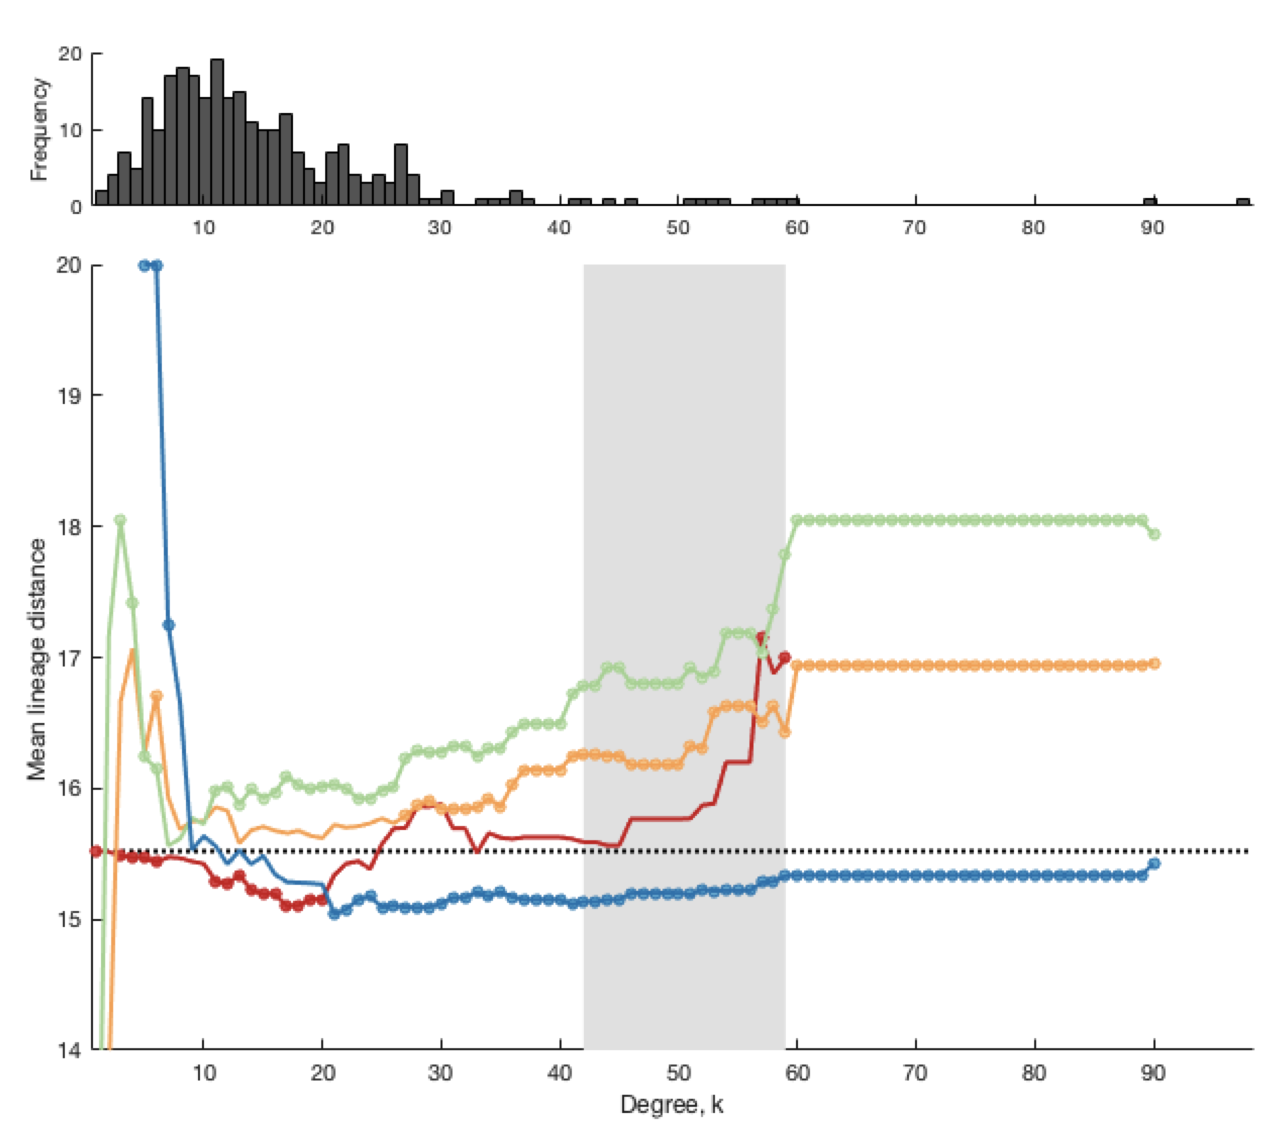
\includegraphics[width=0.7\textwidth]{LineageRFP}
 %\caption{\textbf{}
 %\label{Lineage}
 %\end{figure}

% Place tables after the first paragraph in which they are cited.
% \begin{table}[!ht]
% \begin{adjustwidth}{-2.25in}{0in} % Comment out/remove adjustwidth environment if table fits in text column.
% \centering
% \caption{
% {\bf Table caption Nulla mi mi, venenatis sed ipsum varius, volutpat euismod diam.}}
% \begin{tabular}{|l+l|l|l|l|l|l|l|}
% \hline
% \multicolumn{4}{|l|}{\bf Heading1} & \multicolumn{4}{|l|}{\bf Heading2}\\ \thickhline
% $cell1 row1$ & cell2 row 1 & cell3 row 1 & cell4 row 1 & cell5 row 1 & cell6 row 1 & cell7 row 1 & cell8 row 1\\ \hline
% $cell1 row2$ & cell2 row 2 & cell3 row 2 & cell4 row 2 & cell5 row 2 & cell6 row 2 & cell7 row 2 & cell8 row 2\\ \hline
% $cell1 row3$ & cell2 row 3 & cell3 row 3 & cell4 row 3 & cell5 row 3 & cell6 row 3 & cell7 row 3 & cell8 row 3\\ \hline
% \end{tabular}
% \begin{flushleft} Table notes Phasellus venenatis, tortor nec vestibulum mattis, massa tortor interdum felis, nec pellentesque metus tortor nec nisl. Ut ornare mauris tellus, vel dapibus arcu suscipit sed.
% \end{flushleft}
% \label{table1}
% \end{adjustwidth}
% \end{table}


%PLOS does not support heading levels beyond the 3rd (no 4th level headings).

% \subsubsection*{3rd level heading}
% Text.
%
% \begin{enumerate}
%     \item{react}
%     \item{diffuse free particles}
%     \item{increment time by dt and go to 1}
% \end{enumerate}
%
%
% \subsection*{Another subsection}
%
%
% \begin{itemize}
%     \item First bulleted item.
%     \item Second bulleted item.
%     \item Third bulleted item.
% \end{itemize}

\section*{Discussion}
\begin{itemize}
    \item{First coexpression analysis in worm. Despite noisy gene expression data we get some insights into the genetic basis of connectivity on a neuronal level}
\end{itemize}

% COMPARE TO MOUSE
Compared to our previous work in the mesoscale mouse connectome \cite{Fulcher:2016ck}, the present findings in a near-fully mapped neuronal chemical connectome show similarities and differences.
Despite the incredible difference in spatial scale (from each node containing $\tilde 10^5$ neurons in mouse, to just a single neuron in worm), we found a similar basic qualitative signal of increased coexpression in connected pairs of neurons, and amongst connected pairs, the most similar expression signatures in pairs of connected hub neurons.
These overall findings were specific to connections involving interneurons, i.e., were not found in motor or sensory neurons, being driven by the relatively expression similarity of high-degree interneuron hubs, were not driven by similarity in lineage, neurotransmitter type, or modular membership, and were robust to a range of data processing choices (including connectome type, and coexpression measure).
These findings come despite sparsely annotated, binary gene expression data, with less than 5\% coverage of the full genome, with preliminary enrichment analysis indicating a role for glutamate in both connectivity and hub-connectivity.
Our results indicate that even in a highly specialized neuronal nervous system, costly hub-hub connections display a distinctive transcriptional signature that may reflect their unique functional role in the network.
Further work across different species and scales may shed light on deeper principles of how connectomes organize to facilitate efficient biological functioning.


differ significantly (being a neuronal connectome), and with so few neurons, each highly specialized, it may be hard to pick up broad expression patterns that are network topology-specific.
Quite different to the case in mouse, where regions were spread across the brain, and so effects of regional specialization of function, cytoarchitecture, gene expression were averaged, and the remaining hub-related signal could be isolated.


Being a EM connectome, avoids statistical estimation of connectomes from tract-tracing experiments \cite{Ypma:2016em}, inference of axonal connectivity from diffusion MRI, or the need to form a discrete parcellation of a continuous brain.

[[delete?:]]
[[It has been shown that cells with identical fates can be formed by different gene regulatory pathways \cite{Liu2009} [[relevance?]], however to the best of knowledge the relationship between neuron lineage distance and gene expression patterns has not been investigated yet [[move to discussion?]].]]

% Introduce gene expression work and prior work relating them
The recent availability of gene expression data in the brain has allowed structural connectome properties to be related to molecular information \cite{vandenHeuvel:2017ex}.
% , facilitating cross-scale understanding between the fields of macroscale connectomics and microscale neuroscience \cite{vandenHeuvel:2017ex}.
Initial statistical work done using binary gene expression annotations in \emph{C. elegans} showed that the expression of a small number of genes can be used to predict connectivity between pairs of neurons \cite{Varadan:2006ek, Kaufman2006, Baruch2008b}.
Later work, utilizing detailed quantitative gene expression data in mouse from the Allen Mouse Brain Atlas \cite{Lein:2007jn} revealed a relationship between gene expression and connectivity in mouse \cite{Ji:2014jw, Fakhry:2015kl}, with pairs of brain regions with similar gene expression patterns also displaying similar connectivity profiles (using connectivity data from rat) \cite{French2011}.
% Fakhry:2015dg
% that connected pairs of brain regions display more similar gene expression profiles \cite{French2011},
Comparing different types of connections in mouse, we have demonstrated that pairs of connected hubs have the most similar gene expression profiles, and that hub connectivity is associated with the correlated expression of genes related to oxidative energy metabolism \cite{Fulcher:2016ck}.
Similar findings have been reported at the regional level in the human cortex, with integrative hub regions (with high inter-modular degree and long connection distance) being associated with expression of genes regulating oxidative metabolism and mitochondria \cite{Vertes2016a}.
Both results are consistent with the high metabolic cost of hubs \cite{Collin:2014kq, Tomasi:2013kl}, which may be due to the high signal traffic they're thought to mediate \cite{vandenHeuvel:2012kh, Misic:2014it}, painting a picture of hubs as a highly conserved and metabolically costly feature of structural brain networks.
% These findings highlight a close relationship between metabolic expenditure and the high signaling load of hub regions in the brain, as has been previously proposed \cite{Bullmore2012}.
% As well as being a highly conserved structural feature, these studies hint that hub connectivity may also be consistently related to metabolic demand, with the picture of highly connected hubs being both metabolically costly, both to construct and to run.

% LINEAGE
[[TODO: add details on lineage]] While the relationship between cell lineage and gene expression was studied in other species \cite{Cui2007, Kluger2004}.

LIMITATIONS:
\begin{itemize}
    \item Did the best we had with sparsely-annotated binary gene expression data
    \item No way of discriminating between missing data and the absence of expression
    \item only around 5 percent of genes in the genome available
    \item annotation problems: different qualifiers, loosing sensitivity/specificity if including too much or too little - need to balance
    \item Future work may have actual high-throughput RNAseq gene data for all neurons, could do this analysis properly!
    \item Would surely allow more subtle understanding of how gene expression varies with connectivity roles
\end{itemize}

% Binary expression data
Compared to continuous expression information provided from techniques like RNA sequencing, \emph{in situ} hybridization, or microarray with whole-brain coverage using a systematic experimental procedure \cite{Lein:2007jn, Shen:2012ua, Tasic:2016jp}, the data analyzed here presents numerous challenges.
With access to only a relatively limited coverage of the genome (948 out of $>$19 000 genes \cite{Hillier2005} annotated in the current dataset) [[TODO: how many worm genes in total? Add proportion of worm genes represented ``19,735 protein-coding genes—with $>$90\% directly supported by experimental evidence—and $>$1300 noncoding RNA genes \cite{Hillier2005}'']], the enrichment results provided here are severely constrained in scope.
Further, using the current data, we are unable to distinguish expression levels between neurons that express a given gene, and we are unable to distinguish missing data, from negative data (both are represented as `0' in our data).
Future work systematically mapping gene expression in a unified experimental paradigm would allow a more subtle and comprehensive analysis of gene expression and function.

Thus, despite minimal gene coverage (5\% of the total genome), we developed a new method that was able to find interpretable patterns in the existing binary expression data for \emph{C. elegans}, providing clues as to function of genes that may drive molecular differences between topologically different pairs of neurons.

% Although our data provide indications of which functional gene categories may be relevant, rather than strong statistical confidence,
Our results are broadly consistent with expectations.
For example, as the majority of hubs are command interneurons, which control forward and backward locomotion, enrichment of genes related to locomotory behavior is sensible.
Furthermore, although we couldn't test the exact gene categories from mouse or human, enrichment of related metabolic processes associated with connectivity and hub connectivity hints at an increase in energy demand as a function of connectivity.
% Moreover, we find an increase in GO category (GO:0042133) which is related to neurotransmitter metabolic process which generally consistent with the findings in mouse.

\section*{Conclusion}

Conclusion text.

\section*{Acknowledgments}
Thanks to Alex Fornito for being a big deal.
We thank WormBase.

\nolinenumbers

% Either type in your references using
% \begin{thebibliography}{}
% \bibitem{}
% Text
% \end{thebibliography}
%
% or
%
% Compile your BiBTeX database using our plos2015.bst
% style file and paste the contents of your .bbl file
% here. See http://journals.plos.org/plosone/s/latex for
% step-by-step instructions.
%


\bibliography{library_ben,library}
% \begin{thebibliography}{10}
%\paragraph*{S1 File.}
%\label{S1_File}
%{\bf Lorem ipsum.}  Maecenas convallis mauris sit amet sem ultrices gravida. Etiam eget sapien nibh. Sed ac ipsum eget enim egestas ullamcorper nec euismod ligula. Curabitur fringilla pulvinar lectus consectetur pellentesque.

%\paragraph*{S1 Video.}
%\label{S1_Video}
%{\bf Lorem ipsum.}  Maecenas convallis mauris sit amet sem ultrices gravida. Etiam eget sapien nibh. Sed ac ipsum eget enim egestas ullamcorper nec euismod ligula. Curabitur fringilla pulvinar lectus consectetur pellentesque.

%\paragraph*{S1 Appendix.}
%\label{S1_Appendix}
%{\bf Lorem ipsum.} Maecenas convallis mauris sit amet sem ultrices gravida. Etiam eget sapien nibh. Sed ac ipsum eget enim egestas ullamcorper nec euismod ligula. Curabitur fringilla pulvinar lectus consectetur pellentesque.


% \end{thebibliography}

\newpage
\section*{Supporting information}
\setcounter{figure}{0} \renewcommand{\thefigure}{S\arabic{figure}}
\renewcommand{\thefigure}{S\arabic{figure}}

\subsection*{Expression annotations from WormBase}

Neuronal gene expression is measured as a binary indicator on WormBase \cite{Harris:2009kd}, based on curated data collated from many individual experiments.

Expression annotations are made either `directly' to individual neurons (when an experiment indicates expression in an individual neuron), or `indirectly' to broader classes of neurons like `interneuron' or `head' (meaning that some members of that class exhibit expression of that gene).
In order to maintain specificity of annotations, we only analyzed `direct' annotations here.

Annotations of gene $G$ to neuron $N$ are also made with varying levels of certainty:
`certain' ($G$ was observed to be expressed in $N$),
`enriched' ($G$ has been found to be enriched in a certain dataset through microarray, RNAseq or proteomic analysis),
`partial' ($G$ was observed to be expressed in some cells of a group of neurons that include $N$),
`blank' (data from studies before 2005),
or `uncertain' ($G$ was sometimes observed to be expressed in $N$, or $G$ was observed to be expressed in a cell that could be $N$).
Our analysis excluded annotations labeled as `uncertain' to avoid including false positives.

\subsection*{Quantifying gene coexpression}

In addition to the mean-square contingency coefficient, $r_\phi$, used throughout this work, we also compared a range of alternative similarity measures for binary strings, including the
Jaccard index, $n_{11}/(n_{10}+n_{01}+n_{11})$,
Yule's Q coefficient, $(n_{00}n_{11} - n_{01}n_{10})/(n_{00}n_{11} + n_{01}n_{10})$,
and the $\chi^2$ index, $N (n_{00}n_{11} - n_{01}n_{10})/(n_{1\bullet}n_{0\bullet}n_{\bullet 0}n_{\bullet 1})$ \cite{Kaufman2006}, where $n_{xy}$ counts the number of observations of each of the four binary pairwise possibilities: $n_{00}$, $n_{01}$, $n_{10}$, and $n_{11}$ (as outlined in the main text), while the symbol $\bullet$ sums across a given variable (e.g., $n_{\bullet 0} = n_{00} + n_{10}$).
% and Simple matching coefficients [[TODO: define and give reference]],

Given the sparsity of expression annotation in the data analyzed here, we performed numerical tests to ensure that the coexpression measure used here was not highly sensitive to the proportion of genes expressed in each neuron (i.e., that there was no systematic bias in coexpression with the number of expressed genes in each neuron).
To evaluate each measure, we generated random binary vectors of length 948 containing different proportions of 1s seen in our data, ranging from the minimum, 1, to a maximum, 150, [[Is this actually the max in our data?]].
For all pairwise combinations of proportions, we computed the coexpression measure, taking an average across 1\,000 permutations, and then recorded the resulting mean correlation value, as plotted in Fig.~\ref{fig:S_propOnes}.
Because all vectors are independent random binary strings, the mean coexpression value should be zero in the absence of bias.
We see that the Pearson correlation (Fig.~\ref{fig:S_propOnes}A) shows no systematic bias to the proportion of ones in the vector (varying within $\approx 10^{-3}$), whereas Yule's Q coefficient shows a negative bias for small annotation proportions (Fig.~\ref{fig:S_propOnes}B), while the Jaccard index shows a strong positive bias across the full range (Fig.~\ref{fig:S_propOnes}C).
Based on these numerical experiments, we selected Pearson's mean square contingency coefficient, $r_\phi$, here, to ensure that changes in coexpression were due to matching structure and not simply the number of gene annotations.
% In contrast, other measures such as Jaccard and Yule's index are highly dependent on this ratio (see S1 Fig.).% done with compareProportions script
% and Simple matching coefficients
% For example, Yule's Q, Yule's Y coefficients on average tend to reach extreme values when the ratio between the number of ones and zeros in a vector is large (e.g., 1:20).
% Simple matching coefficient, on the other hand, shows a steady increase with increasing ratio.
% We therefore selected $r_\phi$ to analyze in this work, which was insensitive to the proportion of genes expressed in each neuron.

%% enrichment table for connected links
% results generated using ermineJ, all categories tested separately. significante threshold pcorrected<0.05. Results arranged using

\paragraph*{S1 Table}
{\bf Hub neurons of the \textit{C. elegans} connectome.}
\begin{table}[h]
\centering
\caption{Hub neurons of the \textit{C. elegans} connectome.
Hubs are defined as neurons with $k>41$.
For each hub, we list the neuron name, degree, $k$, location, and function.
Entries have been sorted (descending) by degree.}
\label{tab:HubList}
\begin{tabular}{lll}
\hline
\textbf{Neuron} & \textbf{Degree, $k$} & \textbf{Function}                         \\ \hline
AVAR   & 137        & Head interneuron, role in locomotor decisions                \\
AVAL   & 134        & Head interneuron, role in locomotor decisions                \\
AVBR   & 104        & Head interneuron, role in locomotor decisions                \\
AVBL   & 102        & Head interneuron, role in locomotor decisions                \\
PVCR   & 69         & Tail interneuron, role in locomotor decisions                \\
PVCL   & 64         & Tail interneuron, role in locomotor decisions                \\
AVDR   & 63         & Head interneuron, role in locomotor decisions 				\\
AVER   & 63         & Head interneuron, role in locomotor decisions                \\
AVEL   & 62         & Head interneuron, role in locomotor decisions                \\
DVA    & 59         & Head interneuron, mechanosensory integration                \\
RIBL   & 56         & Head interneuron                							\\
AVKL   & 53         & Head interneuron                                             \\
AVDL   & 52         & Head interneuron, role in locomotor decisions                 \\
RIBR   & 52         & Head interneuron                                             \\
AIBR   & 49         & Head interneuron                                             \\
RIGL   & 49         & Head interneuron                                             \\\hline
\end{tabular}
\end{table}


\paragraph*{S2 Table}
{\bf Enrichment results for connected \textit{vs} unconnected neurons.}
\begin{table}[]
\centering
\caption{Biological processes GO categories showing increased gene coexpression for connected neurons compared to unconnected neurons.
Categories that remain significant after false discovery rate ($P_\mathrm{FDR} < 0.05$) correction are shown boldface.
Entries have been sorted (descending) by uncorrected $P$-value.}
\label{enrichmentCON}
\begin{tabular}{llll}
\hline
\textbf{GOcategory} 	& \textbf{Description}                                     & \textbf{No. of genes} & \textbf{Pval} \\ \hline
\underline{GO:0035235} & ionotropic glutamate receptor signaling pathway & 7        & 1e-12   \\
\underline{GO:0007215} & glutamate receptor signaling pathway         & 9       & 3e-05   \\
GO:0007166 & cell surface receptor signaling pathway         & 48       & 0.00242 \\
GO:0006950 & response to stress                              & 62       & 0.00514 \\
GO:0007613 & memory                                          & 5        & 0.00525 \\
GO:0034220 & ion transmembrane transport                     & 73       & 0.01025 \\
GO:0055085 & transmembrane transport                         & 87       & 0.01035 \\
GO:0040009 & regulation of growth rate                       & 8        & 0.0124  \\
GO:0040010 & positive regulation of growth rate              & 8        & 0.0124  \\
GO:0006811 & ion transport                                   & 93       & 0.01287 \\
GO:0006972 & hyperosmotic response                           & 8        & 0.01687 \\
GO:0009266 & response to temperature stimulus                & 21       & 0.01704 \\
GO:0002376 & immune system process                           & 8        & 0.01829 \\
GO:0006979 & response to oxidative stress                    & 9        & 0.0188  \\
GO:0006970 & response to osmotic stress                      & 11       & 0.02435  \\\hline
\end{tabular}
\end{table}


\paragraph*{S3 Table.}
{\bf Enrichment results for chemical links.}

\begin{table}[]
\centering
\caption{Biological processes GO categories showing increased gene coexpression for chemical links compared all other links.}
\label{enrichmentChemical}
\begin{tabular}{llll}
\hline
\textbf{GOcategory} & \textbf{Description}                                     & \textbf{No. of genes} & \textbf{P value}    \\ \hline
GO:0007292 & female gamete generation                                                                                      & 10       & 0.0003  \\
GO:0048477 & oogenesis                                                                                                     & 10       & 0.0003  \\
GO:0007281 & germ cell development                                                                                         & 12       & 0.00075 \\
GO:0022412 & \begin{tabular}[c]{@{}l@{}}cellular process involved in reproduction\\ in multicellular organism\end{tabular} & 12       & 0.00075 \\
GO:0044711 & single-organism biosynthetic process                                                                          & 27       & 0.00142 \\
GO:0032268 & regulation of cellular protein metabolic process                                                              & 20       & 0.00168 \\
GO:0051246 & regulation of protein metabolic process                                                                       & 20       & 0.00168 \\
GO:1901617 & organic hydroxy compound biosynthetic process                                                                 & 7        & 0.00321 \\
GO:0019752 & carboxylic acid metabolic process                                                                             & 10       & 0.00345 \\
GO:0006464 & cellular protein modification process                                                                         & 51       & 0.00357 \\
GO:0036211 & protein modification process                                                                                  & 51       & 0.00357 \\
GO:0019538 & protein metabolic process                                                                                     & 80       & 0.00376 \\
GO:0007276 & gamete generation                                                                                             & 16       & 0.00445 \\
GO:0006082 & organic acid metabolic process                                                                                & 11       & 0.00449 \\
GO:0043436 & oxoacid metabolic process                                                                                     & 11       & 0.00449\\ \hline
\end{tabular}
\end{table}

\paragraph*{S4 Table.}
{\bf Enrichment results for electrical links.}

\begin{table}[]
\centering
\caption{Biological processes GO categories showing increased gene coexpression for electrical links compared to all other links.}
\label{enrichmentElectrical}
\begin{tabular}{llll}
\hline
\textbf{GOcategory} & \textbf{Description}                                     & \textbf{No. of genes} & \textbf{P value}    \\ \hline
GO:0040034 & regulation of development, heterochronic                                                             & 7        & 0.00083 \\
GO:0006417 & regulation of translation                                                                            & 5        & 0.00415 \\
GO:0016441 & posttranscriptional gene silencing                                                                   & 5        & 0.00415 \\
GO:0016458 & gene silencing                                                                                       & 5        & 0.00415 \\
GO:0031047 & gene silencing by RNA                                                                                & 5        & 0.00415 \\
GO:0034248 & regulation of cellular amide metabolic process                                                       & 5        & 0.00415 \\
GO:0035194 & posttranscriptional gene silencing by RNA                                                            & 5        & 0.00415 \\
GO:0040029 & regulation of gene expression, epigenetic                                                            & 5        & 0.00415 \\
GO:0051932 & synaptic transmission, GABAergic                                                                     & 5        & 0.00589 \\
GO:0032269 & \begin{tabular}[c]{@{}l@{}}negative regulation of cellular protein \\ metabolic process\end{tabular} & 10       & 0.00637 \\
GO:0051248 & negative regulation of protein metabolic process                                                     & 10       & 0.00637 \\
GO:0008361 & regulation of cell size                                                                              & 12       & 0.00848 \\
GO:0010608 & posttranscriptional regulation of gene expression                                                    & 6        & 0.00902 \\
GO:0010558 & \begin{tabular}[c]{@{}l@{}}negative regulation of macromolecule \\ biosynthetic process\end{tabular} & 13       & 0.00935 \\
GO:0032535 & regulation of cellular component size                                                                & 13       & 0.00935 \\ \hline
\end{tabular}
\end{table}

\paragraph*{S5 Table.}
{\bf Enrichment results for links involving hubs.}

\begin{table}[]
\centering
\caption{Biological processes GO categories showing increased gene coexpression for links involving hubs (rich, feed-in and feed-out) compared to peripheral links.}
\label{enrichmentRF}
\begin{tabular}{llll}
\hline
\textbf{GOcategory} & \textbf{Description}                                           & \textbf{No. of genes} & \textbf{P value} \\
\hline
\underline{GO:0035235} & ionotropic glutamate receptor signaling pathway                         & 7            & 1e-12   \\
\underline{GO:0007215} & glutamate receptor signaling pathway                                    & 9            & 1e-05   \\
\underline{GO:0034220} & ion transmembrane transport                                             & 63           & 0.00025 \\
\underline{GO:0055085} & transmembrane transport                                                 & 75           & 0.0003  \\
\underline{GO:0006811} & ion transport                                                                                                      & 80           & 0.00041 \\
GO:0045935 & \begin{tabular}[c]{@{}l@{}}positive regulation of nucleobase-containing \\ compound metabolic process\end{tabular} & 30           & 0.00402 \\
GO:0040012 & regulation of locomotion                                                                                           & 51           & 0.00406 \\
GO:0007166 & cell surface receptor signaling pathway                                                                            & 44           & 0.0041  \\
GO:0007267 & cell-cell signaling                                                                                                & 43           & 0.00482 \\
GO:0009891 & positive regulation of biosynthetic process                                                                        & 31           & 0.0049  \\
GO:0031328 & positive regulation of cellular biosynthetic process                                                               & 31           & 0.0049  \\
GO:0051173 & \begin{tabular}[c]{@{}l@{}}positive regulation of nitrogen compound \\ metabolic process\end{tabular}              & 31           & 0.0049  \\
GO:0007268 & chemical synaptic transmission                                                                                     & 36           & 0.00556 \\
GO:0098916 & anterograde trans-synaptic signaling                                                                               & 36           & 0.00556 \\
GO:0099536 & synaptic signaling                                                                                                 & 36           & 0.00556 \\\hline
\end{tabular}
\end{table}


% Please add the following required packages to your document preamble:
% \usepackage[normalem]{ulem}
% \useunder{\uline}{\ul}{}

% ------------------------------------------------------------------------------
% Include only the SI item label in the paragraph heading. Use the \nameref{label} command to cite SI items in the text.
% ------------------------------------------------------------------------------

% ------------------------------------------------------------------------------
% compare proportions for simulations to validate
% ------------------------------------------------------------------------------
% \paragraph*{S1 Fig.}
% {\bf Comparing different coexpression measures.}
\begin{figure}[h]
\centering
    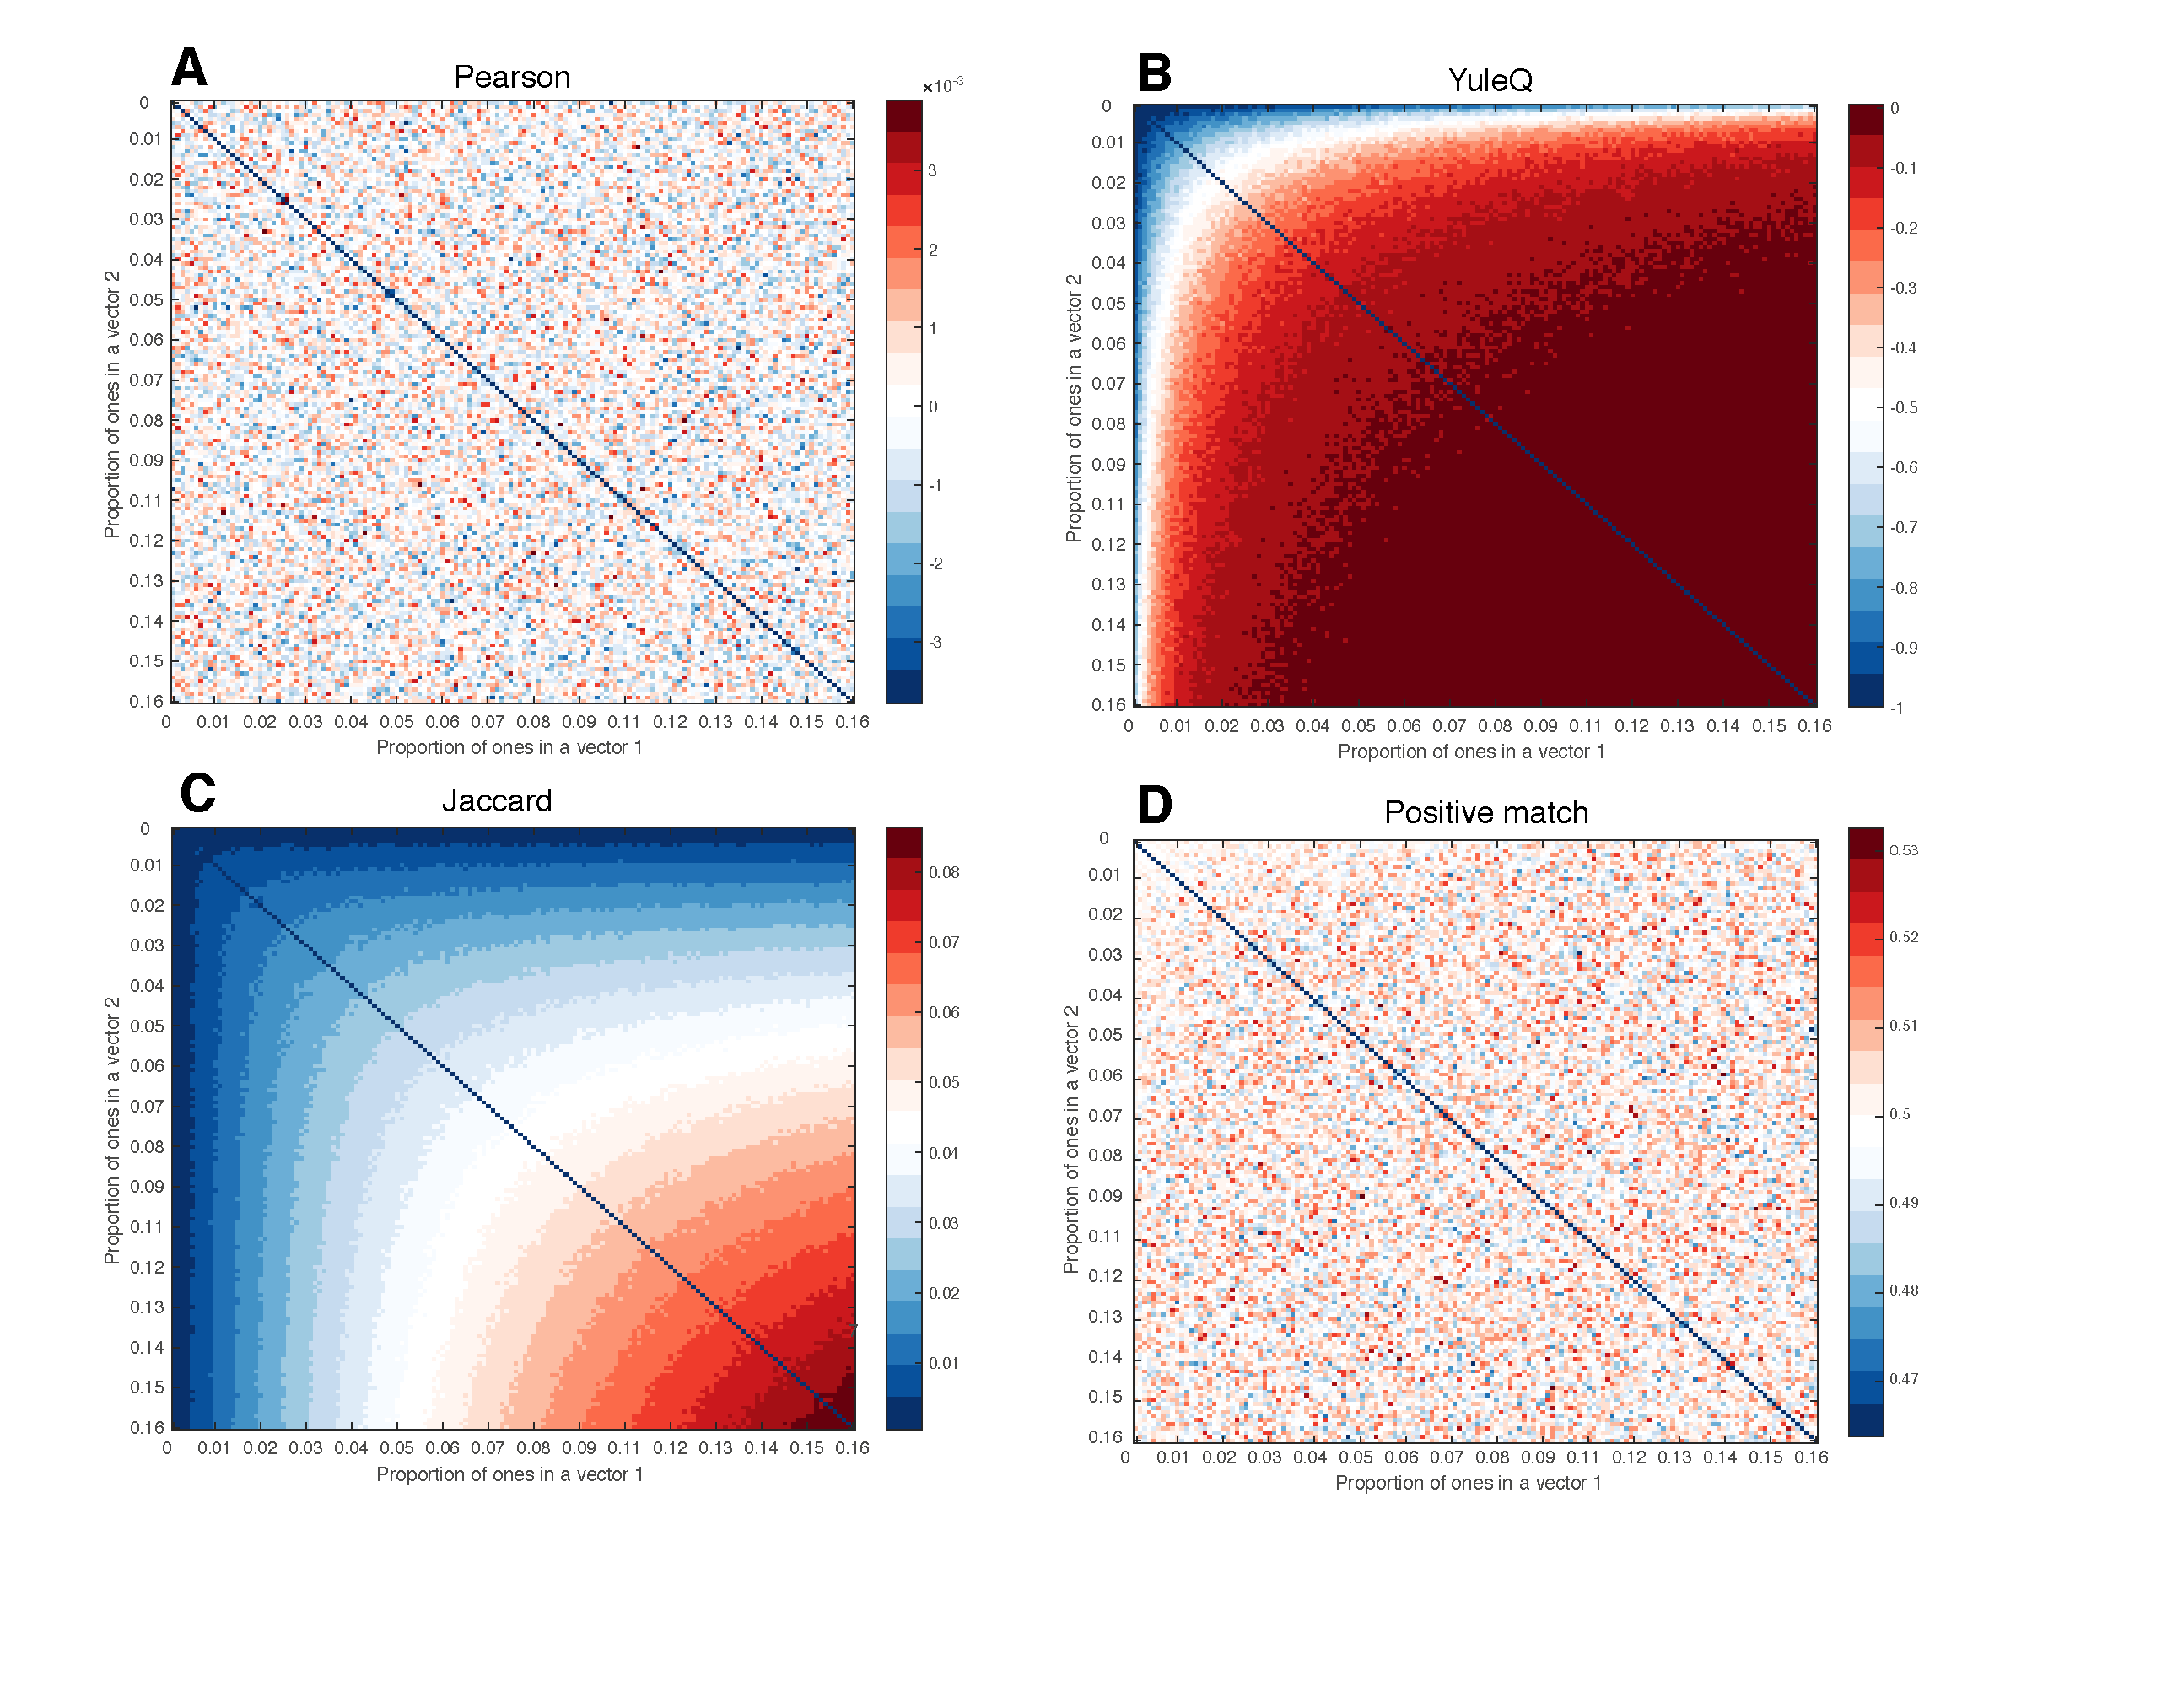
\includegraphics[width=1\textwidth]{CoexpressionMeasures.pdf}
\caption{
\label{fig:S_propOnes}
\textbf{Dependence of binary coexpression metrics on the proportion of positive annotations.}
% Given the sparse binary annotation of genes to neurons, we investigated bias in each measure across 1\,000 pairs of random binary vectors, each with a fixed proportion of ones.
Shown here is the mean correlation between pairs of random, binary vectors of length 948, with different proportions of 1s (between 0--0.16; matrix size is 150$\times$150, therefore the number of ones ranges from 1 to 150).
Each point is averaged over 1\,000 different pairs of random vectors (or just 100 runs in the case of the positive match measure, which is more computationally intensive to compute).
 % for 948-long vectors with between 0--0.16 proportion of ones (matrix size is 150x150, therefore the number of ones ranges from 1 to 150).
Bias is indicated by a systematic trend in correlation values, driven simply by the proportion of positive annotations for a pair of vectors.
\textbf{A} Pearson, $r_\phi$, the measure used throughout this work, shows no systematic bias (note the color axis scale, 10$^{-3}$).
By contrast, the remaining measures to show a dependence on the proportion of 1s in each vector:
\textbf{B} Jaccard[[TODO: JACCARD WHAT?]],
\textbf{C} Yule's $Q$, and
\textbf{D} Positive match probability, Eq.~\ref{eqn:positiveMatch}.
}
\end{figure}


% \paragraph*{S2 Fig.}
% {\bf Connection probability decreases with the separation distance between neurons}
% ------------------------------------------------------------------------------
% <<probabilityVSdistance>>
% ------------------------------------------------------------------------------
\begin{figure}[h]
\centering
    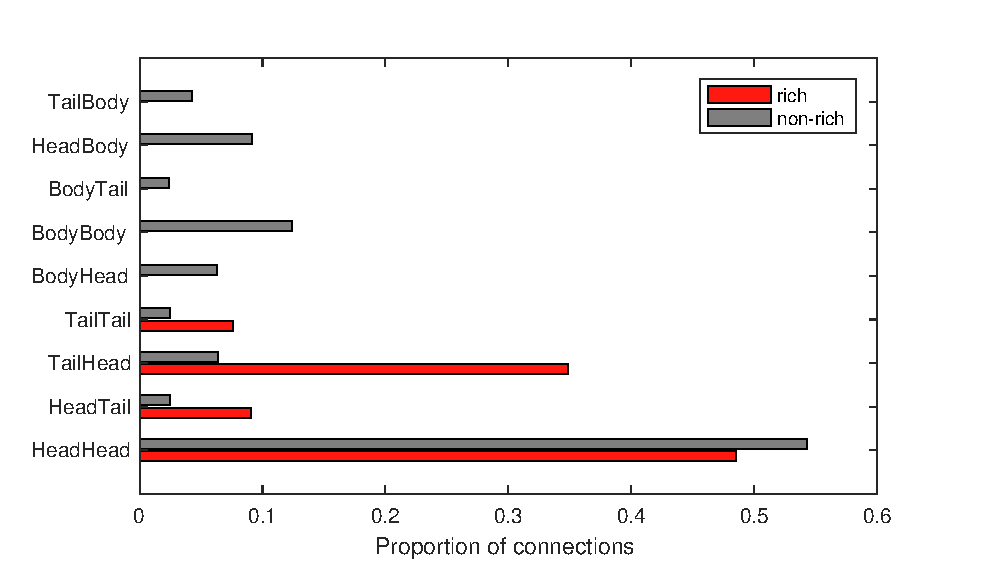
\includegraphics[width=1\textwidth]{connectionProportionDivision.eps}
\caption{
\label{fig:S_connectionProportion}
Distribution of hub-hub connections (`rich', red), and all other connections (`non-rich', i.e., feeder and peripheral, gray) across anatomical divisions (head, body, and tail), defining hubs as those with degree, $k > 41$, corresponding to the lowest threshold at which the \emph{C. elegans} connectome exhibits rich-club organization.
The increased separation distance between hubs is driven by a relative increase in connection density between the head and tail.
}
\end{figure}
% ------------------------------------------------------------------------------

% ------------------------------------------------------------------------------
% <<plot_coexpDistance.m>>
% [[coexpressionDistance(C,G),CoExpressionDistanceDetail(C,G)]]
% ------------------------------------------------------------------------------
% \paragraph*{S3 Fig.}
% {\bf Gene coexpression decreases with separation distance within the head and tail.}
\begin{figure}[h]
\centering
    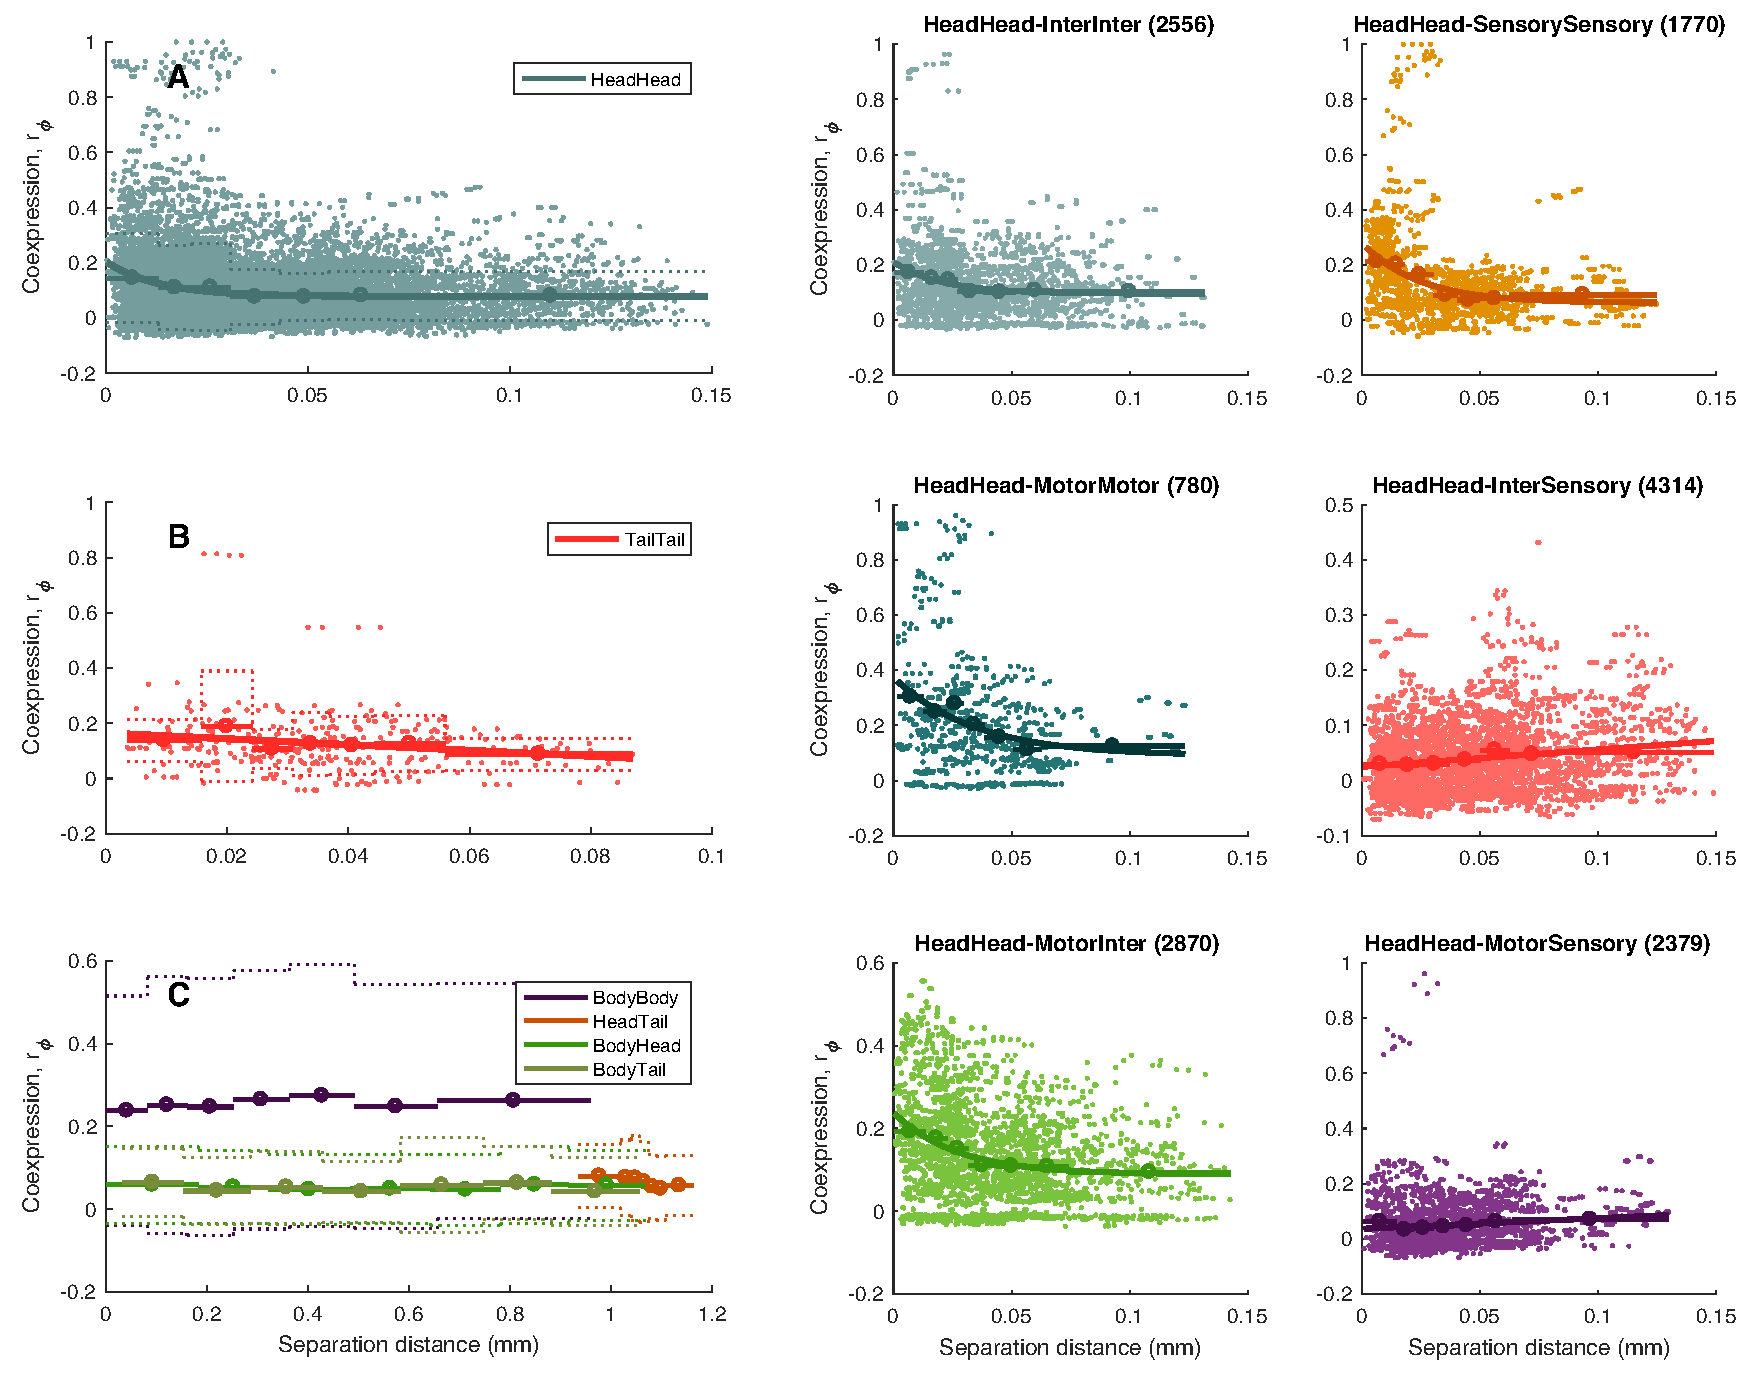
\includegraphics[width=1\textwidth]{DistanceCoexpression.pdf}
    % 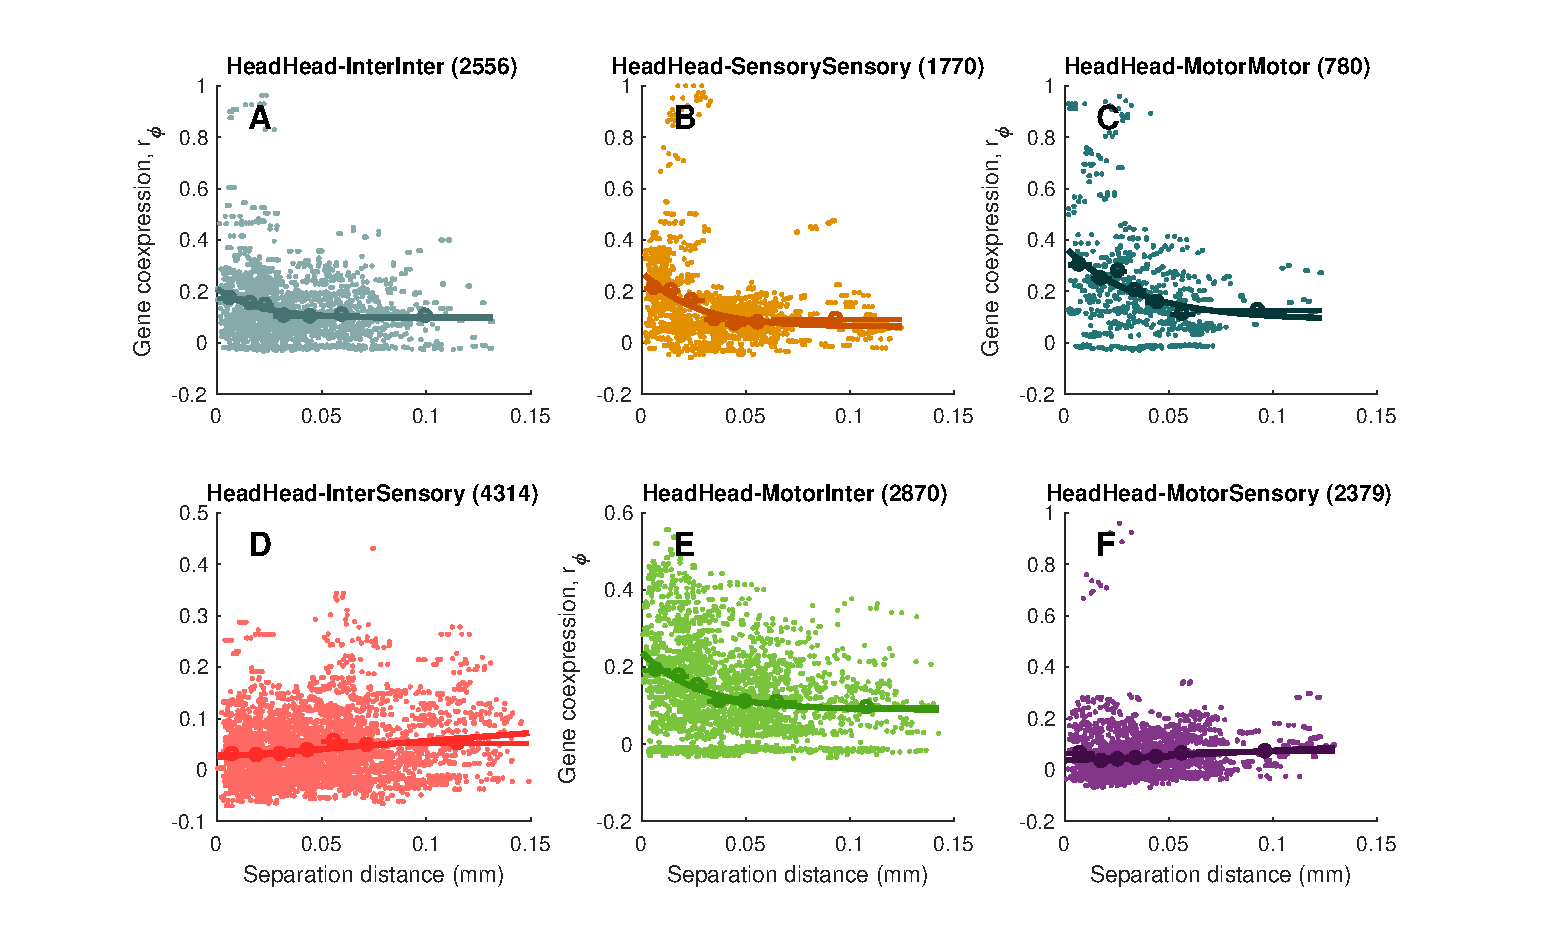
\includegraphics[width=1\textwidth]{coExpressionDistanceDetail.eps}
\caption{
\label{fig:S_distCoexp}
\textbf{Gene coexpression decreases with separation distance within the head and tail.}
Gene coexpression, $r_\phi$ (in all cases excluding left-right homologous pairs of neurons), is shown as a function of the pairwise separation distance between pairs of neurons (shown as the mean (solid) $\pm$ standard deviation (dotted) in seven equiprobable distance bins, with extent shown as horizontal bars), for \textbf{A} all pairs of neurons in the head, \textbf{B} all pairs of neurons in the tail, and \textbf{C} all other pairs (labeled).
Scatters for all neuron pairs are added in \textbf{A} and \textbf{B}.
An exponential relationship, $f(x) = a\exp(-bx)+c$, is fitted in \textbf{A} and \textbf{B}, revealing a slight decreasing trend in $r_\phi$ with distance, as per macroscopic mammalian brains \cite{Fulcher:2016ck, Krienen:2016eq}.
Looking within the head, we find different spatial relationships as a function of neuron type, shown for \textbf{C} pairs of interneurons, \textbf{D} pairs of motor neurons, \textbf{E} motor-interneuron pairs, \textbf{F} pairs of sensory neurons, \textbf{G} interneuron-sensory neuron pairs, and \textbf{H} motor-sensory pairs.
[[TODO: add labels for subplots C--H, label all axes? Change axis label to Gene coexpression, $r_\phi$ ]]
}
\end{figure}
% ------------------------------------------------------------------------------


% ------------------------------------------------------------------------------
% <<FeedInOutNodes.m>>
% ------------------------------------------------------------------------------
% \paragraph*{S4 Fig.}
% {\bf Neuron properties vary in therms of their connectivity relationship to hub nodes. }
\begin{figure}[h]
\centering
    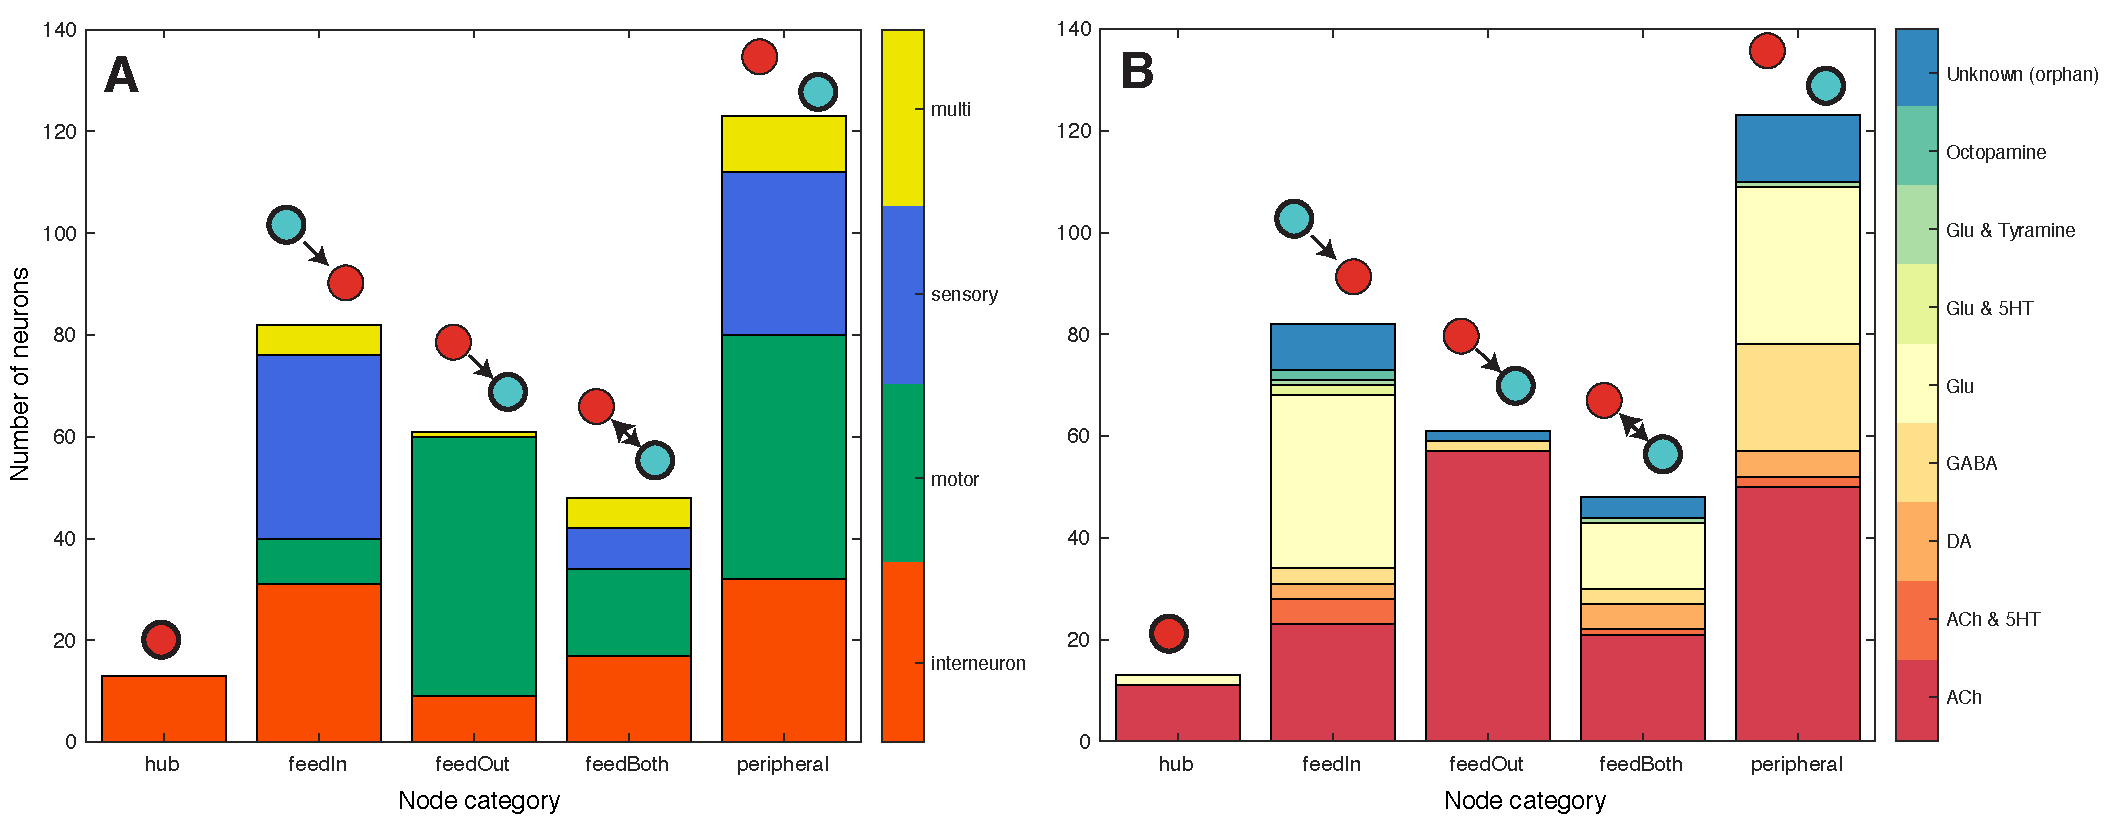
\includegraphics[width=1\textwidth]{FeedInOutNodesJustTwo.pdf}
\caption{
\textbf{Neuron properties vary in terms of their connectivity relationship to hub nodes.}
Using a degree threshold for hubs, $k > 41$, we class all individual neurons into five mutually exclusive categories, shown schematically in the figures, for hubs (red) and nonhubs (light blue), as:
(i) `hub' ($k>41$),
and then classify nonhubs ($k\leq41$) as:
(ii) `feedIn' (projects to a hub, but does not receive a projection from a hub),
(iii) `feedOut' (receives a projection from a hub, but does project to a hub),
(iv) `feedBoth' (receives a projection from, and projects to a hub),
(v) `peripheral' (neither receives a projection from nor projects to a hub).
We show the number of neurons in each of these fives classes that:
\textbf{A} is an interneuron (orange), motor neuron (green), sensory neuron (blue), or multimodal (yellow),
% \textbf{B} is in the head (gray), body (purple), or tail (red),
\textbf{B} uses one of nine neurotransmitter systems (labeled).
\label{fig:S_feedInOutNodes}
[[TODO: Come up with new names for nodes that don't confuse with edge names. Labels not visible for B]]
}
\end{figure}
% ------------------------------------------------------------------------------


% ------------------------------------------------------------------------------
% <<plot_disstributionsSUPP.m>>
% ------------------------------------------------------------------------------

% \paragraph*{S6 Fig.}
% {\bf Coexpression for rich, feeder and peripheral links as a function of degree.}
\begin{figure}[h]
\centering
    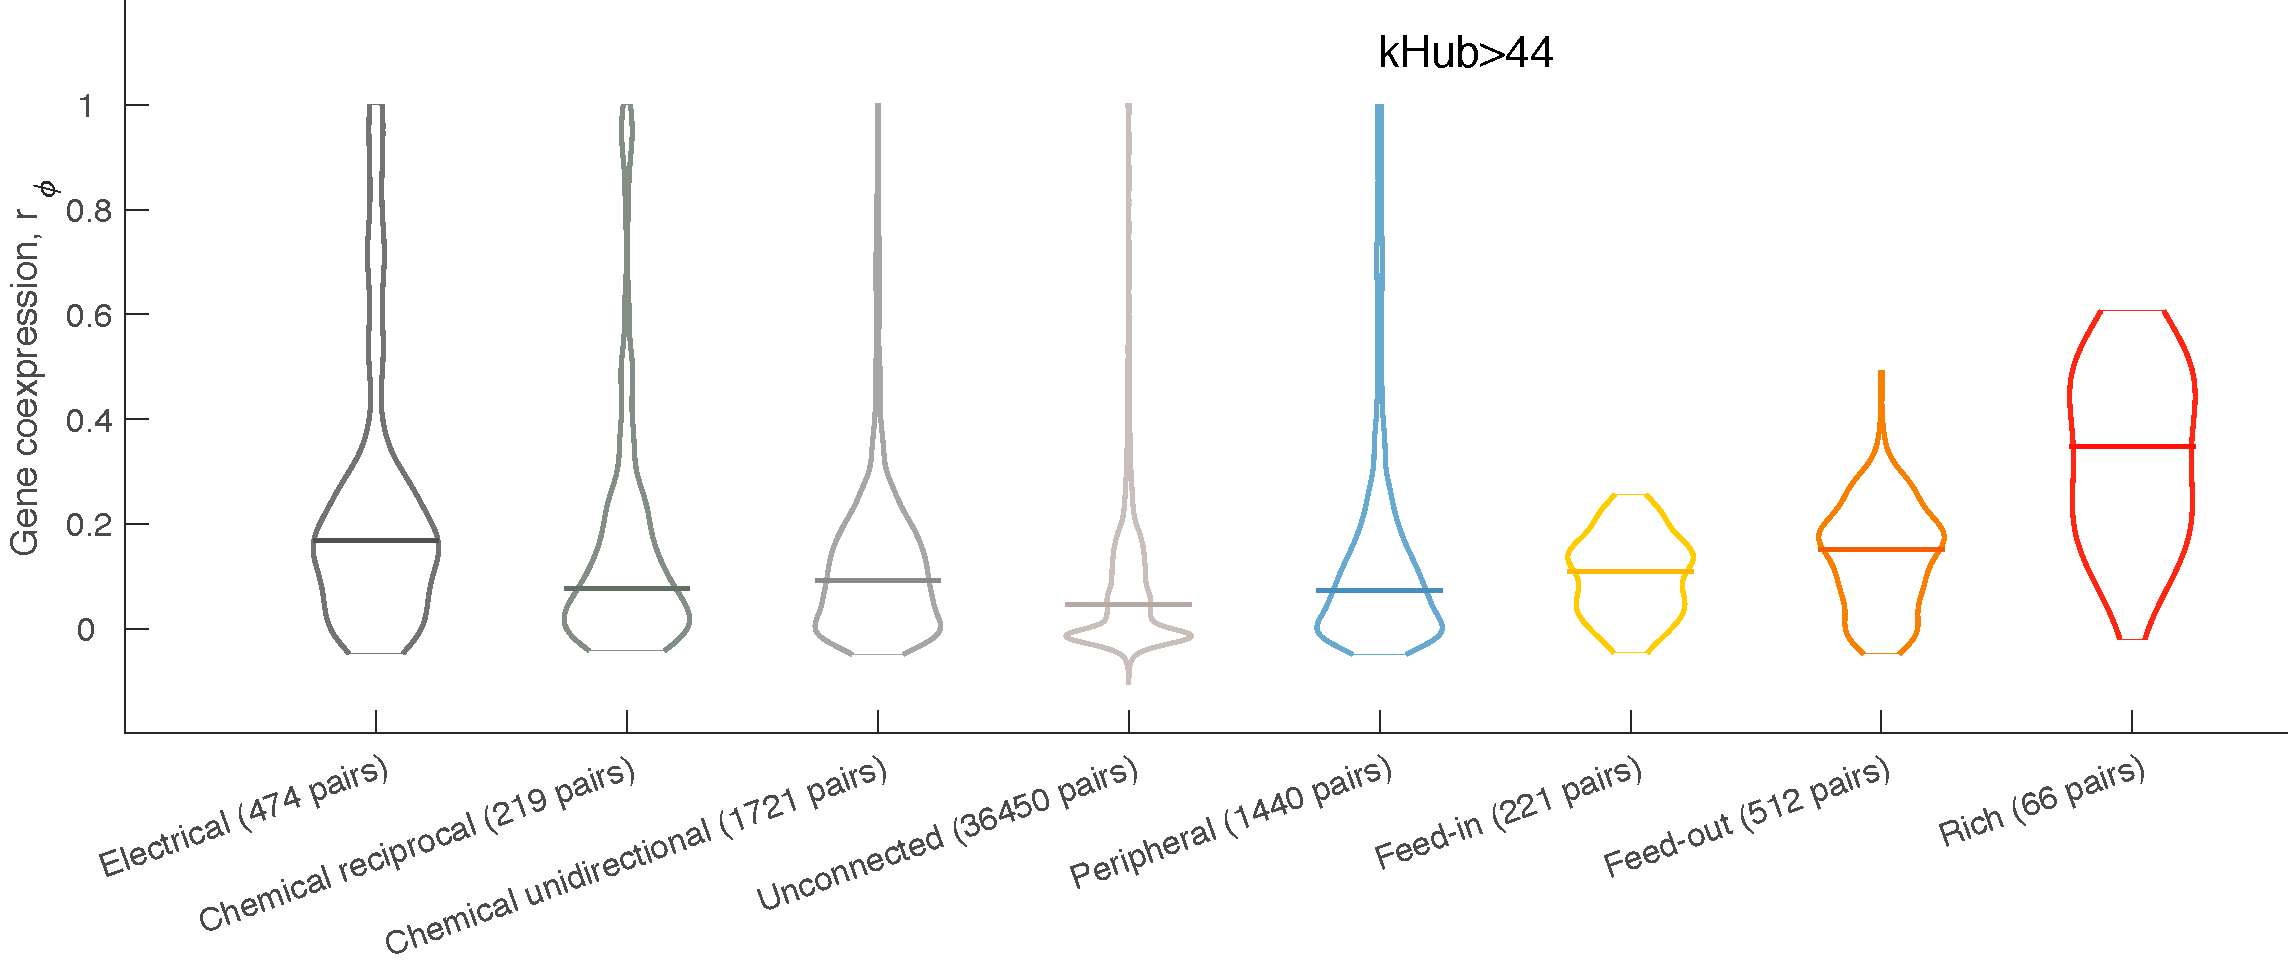
\includegraphics[width=1\textwidth]{distributionsALL.pdf}
    \caption{
\textbf{Coexpression for different types of connectome edges.}
\emph{Left}: Distribution of transcriptional similarity between reciprocally connected (219 pairs), unidirectionally connected (1\,721) and  and unconnected (36\,749 pairs) pairs of neurons as a violin plot, with the median of each distribution shown as a horizontal line.
Connections between symmetrical (left/right) pairs of neurons are excluded from the analysis. Coexpression values for
Coexpression, $r_\phi$ is increased in connected (reciprocally and unidirectionally) pairs of neurons ($P < 10^{-50}$, Wilcoxon rank sum test)
\emph{Right}: Distribution of transcriptional similarity for rich, feed-in, feed-out and peripheral links, where hubs are neurons with degree $k>41$.
[[TODO: color inside of the distributions
Add $p<0.05$ values on the plot where significant.
Use mean instead of median (or use median throughout)
]]
\label{fig:S_RFPdistributions}
}
\end{figure}

% <<networkRC.m>>
% \paragraph*{S7 Fig.}
% {\bf Weighted and mixed rich club}
\begin{figure}[h]
\label{fig:S_weightedRC}
\centering
    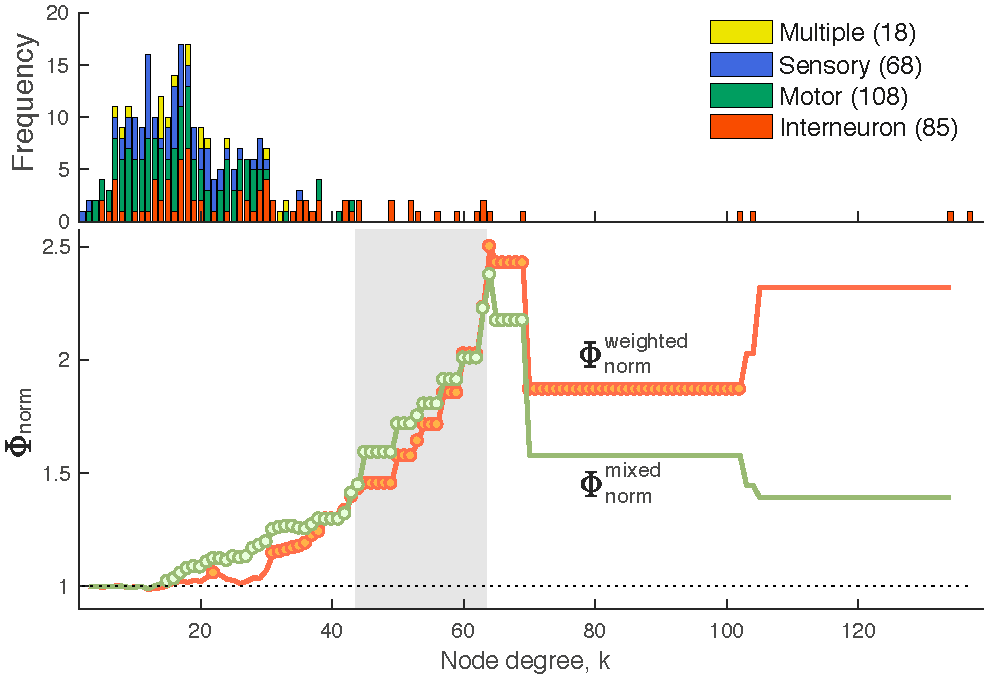
\includegraphics[width=1\textwidth]{weightedRCALL.pdf}
    \caption{\textbf{A} Degree distribution of the binary synaptic connectome, where neurons are labeled according to four categories:
(i) interneuron (85 neurons, orange),
(ii) sensory (68 neurons, blue),
(iii) motor (108 neurons, green), or
(iv) multimodal (18 neurons, yellow).
An extended tail of high-degree neurons can be seen, which are mostly interneurons.
\textbf{B}
Normalized weighted (topology fixed and weights randomized in the null model, shown orange) $\Phi_\mathrm{norm}^\mathrm{weighted}$ and mixed (both topology and weights mixed in the null model, shown green) $\Phi_\mathrm{norm}^\mathrm{mixed}$ rich club coefficient as a function of the degree, $k$, at which hubs are defined (as neurons with degree $>k$).
Circles indicate values of $\Phi_\mathrm{norm}$ that are significantly higher than an ensemble of 1\,000 degree-matched null networks (Welch's $t$-test, $P < 0.05$).
[[TODO: Change the labels within the plot for mixed and weighted as superscripts]]
[[TODO: define/explain the two definitions and give references]]
}
\end{figure}

% ------------------------------------------------------------------------------
% <<RichClub.m>>
% \paragraph*{S8 Fig.}
% {\bf Mean lineage distance as a function of degree for different link types}
\begin{figure}[!h]
\centering
    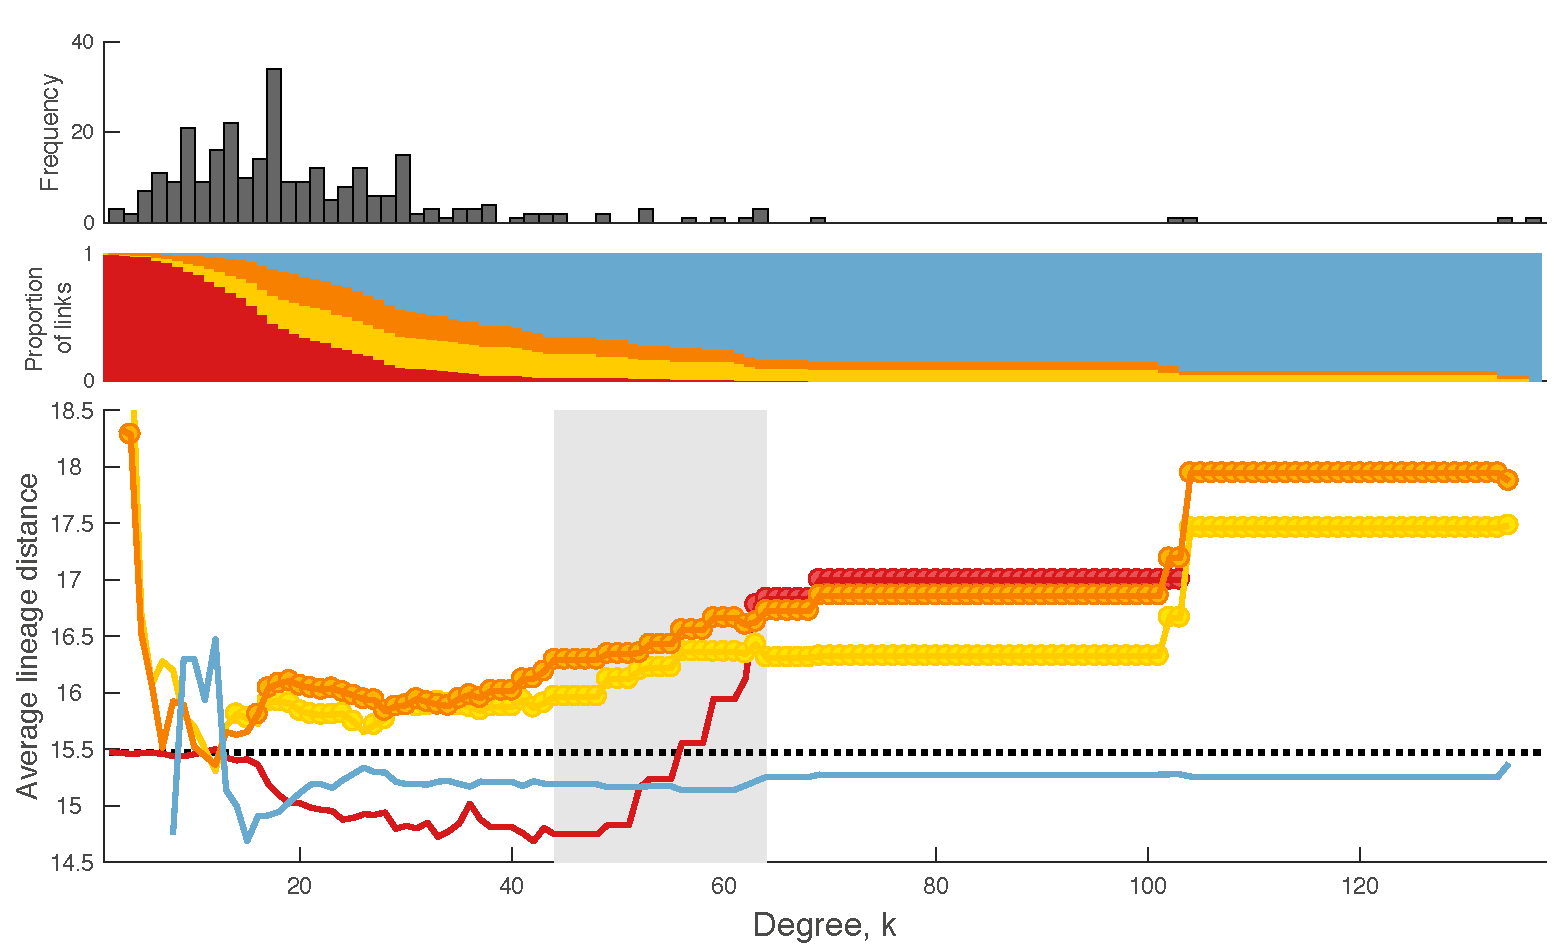
\includegraphics[width=1\textwidth]{lineageDistanceRPF.pdf}
    \caption{
    \textbf{Lineage distance between pairs of neurons for different connection types as a function of the degree at which hubs are defined, $k$.}
    \emph{Top}: Degree distribution.
\emph{Middle}: proportion of connections that are `rich' (hub$\rightarrow$hub, red), `feed-in' (nonhub$\rightarrow$hub, yellow), `feed-out' (hub$\rightarrow$nonhub, orange), and `peripheral' (nonhub$\rightarrow$nonhub, blue) as a function of the degree threshold, $k$, used to define hubs.
Note that at high $k$, most neurons are labeled as nonhubs, and hence the vast majority of connections are `peripheral'.
\emph{Lower}: Mean lineage distance for each connection type as a function of $k$.
Lineage distance across all network links shown as a dotted black line; the topological rich-club regime (determined from the network topology, cf. Fig.~\ref{fig:topology_rich}) is shaded gray.
Circles indicate a statistically significant increase or decrease in birth time difference in a given link type relative to the rest of the network (two-sided Welch’s t test; $P < 0.05$).
}
\label{fig:Lineagek}
\end{figure}
% <<RichClub.m>>

% ------------------------------------------------------------------------------
% \paragraph*{S9 Fig.}
% {\bf Mean birth time difference as a function of degree for different link types}
\begin{figure}[!h]
\label{BirthTimesk}
\centering
    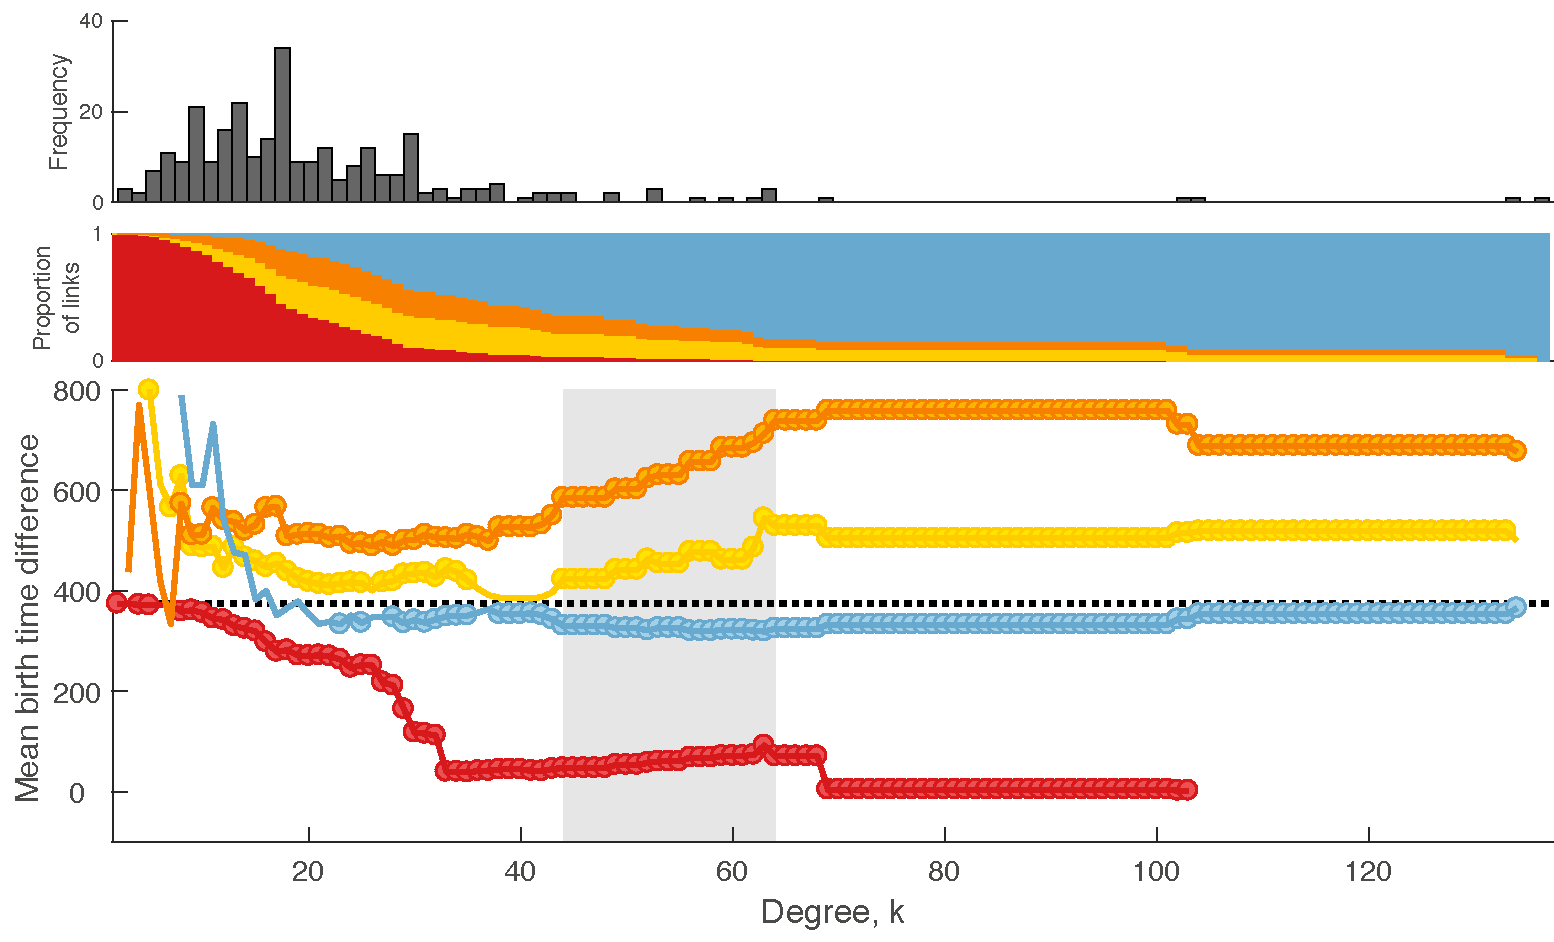
\includegraphics[width=1\textwidth]{birthTimeRPFALL.pdf}
    \caption{
\emph{Top}: Degree distribution.
\emph{Middle}: proportion of connections that are `rich' (hub$\rightarrow$hub, red), `feed-in' (nonhub$\rightarrow$hub, yellow), `feed-out' (hub$\rightarrow$nonhub, orange), and `peripheral' (nonhub$\rightarrow$nonhub, blue) as a function of the degree threshold, $k$, used to define hubs.
Note that at high $k$, most neurons are labeled as nonhubs, and hence the vast majority of connections are `peripheral'.
\emph{Bottom}: Mean birth time difference for each connection type as a function of $k$.
The mean birth time difference across all network links shown as a dotted black line; the topological rich-club regime (determined from the network topology, cf. Fig.~\ref{fig:topology_rich}) is shaded gray.
Circles indicate a statistically significant increase or decrease in birth time difference in a given link type relative to the rest of the network (two-sided Welch's $t$ test; $P < 0.05$).
}
\end{figure}

% propTypesDegree(C) script
%\paragraph*{S6 Fig.}
%{\bf Neuron type and neurotransmitter as a function of degree}
%\begin{figure}[!h]
%\label{S7_Fig}
%\centering
%    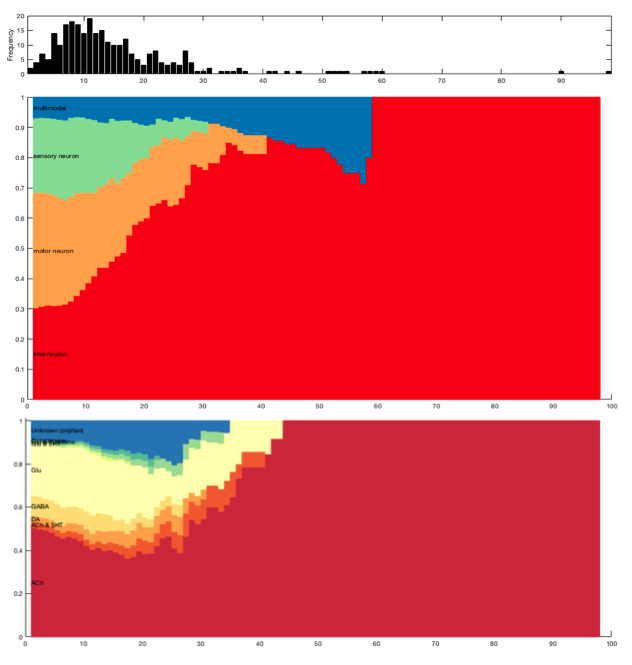
\includegraphics[width=0.7\textwidth]{TypeTransmitterDegree}
%\end{figure}

% RichClub script
% \paragraph*{S10 Fig.}
% {\bf Average coexpression for rich, feeder and peripheral links as a function of degree.}
\begin{figure}[!h]
\label{RFPposmatches}
\centering
    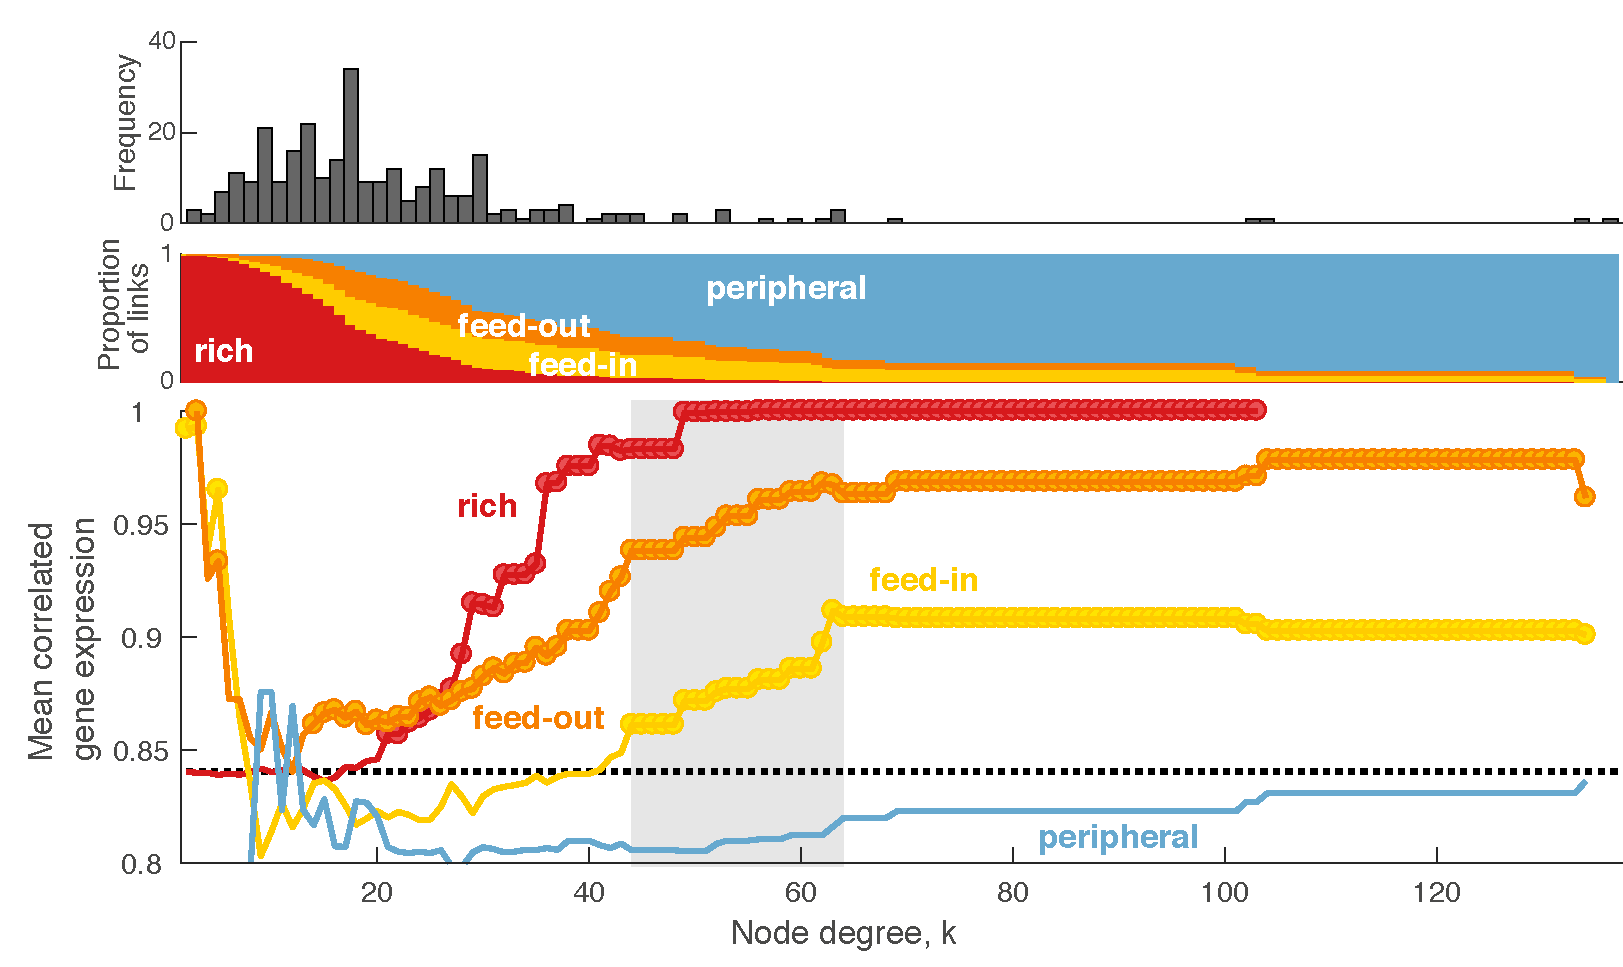
\includegraphics[width=1\textwidth]{meanCoexpressionCoXALL.pdf}
\caption{
\textbf{Gene coexpression, as measured by a positive matching probability index, Eq.~(\ref{eqn:positiveMatch}).}
\emph{Top}: Degree distribution.
\emph{Middle}: proportion of connections that are `rich' (hub$\rightarrow$hub, red), `feed-in' (nonhub$\rightarrow$hub, yellow), `feed-out' (hub$\rightarrow$nonhub, orange), and `peripheral' (nonhub$\rightarrow$nonhub, blue) as a function of the degree threshold, $k$, used to define hubs.
Note that at high $k$, most neurons are labeled as nonhubs, and hence the vast majority of connections are `peripheral'.
\emph{Bottom}: Mean gene coexpression calculated using similarity index from only positive matches, $r_\xi$, for each connection type as a function of $k$.
The mean coexpression across all network links shown as a dotted black line; the topological rich-club regime (determined from the network topology, cf. Fig.~\ref{fig:topology_rich}) is shaded gray.
Circles indicate a statistically significant increase in gene coexpression in a given link type relative to the rest of the network (one-sided Welch's $t$ test; $P < 0.05$).
}
\end{figure}


\end{document}
